%!TEX encoding = IsoLatin

%% Document is article 
\documentclass[a4paper]{report}

%% ----------------------------------------------------- PACKAGES ----------------------------------------------------- %%
\usepackage{coolReport}
\usepackage{algorithm2e}
\usepackage{multirow}
\usepackage{tabularx}
\graphicspath{{./Images/}}
\cRTitle{Semester project report}

%% ---------------------------------------------------------TITLE --------------------------------------------------------- %%

%% ---------------------------------------------------- DOCUMENT ---------------------------------------------------- %%
\begin{document}
	%!TEX encoding = IsoLatin


%% ------------------------------------------------------- PATHS ------------------------------------------------------- %%

%% --------------------------------------------------- PAGE STYLE --------------------------------------------------- %%

%% ---------------------------------------------------- DOCUMENT ---------------------------------------------------- %%


\begin{titlepage}
        	{\sffamily
	\large
        		\noindent \'ECOLE POLYTECHNIQUE FEDERALE DE LAUSANNE \\
        		MT SECTION\\
        		FAURY Louis \\
        	}
	
	\vfill 
        \begin{center}
   		{\sffamily\Huge
         		\textbf{SEMESTER PROJECT REPORT} \\
			\vspace{0.3cm}
			\Large
			\textbf{LASA}
		}
		\vspace{1cm}
	
        		
\includegraphics[width=0.8\textwidth]{epfl_logo.png}
        
        		\vspace{1cm}
         
         	\sffamily\huge\textbf{ 	
\titlebox{0.95}{\sffamily\huge\textbf{Learning from suboptimal demonstrations: the role of compliance in the exploration-exploitation trade-off}} }
        \end{center}
        
	\vspace{2cm}
         \centering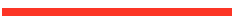
\includegraphics[width=0.1\textwidth]{sepLine}
         \vspace{0.2cm}

	\large
        \begin{center}
		\begin{tabular}{rl}
    			\textbf{Laboratory} & Learning Algorithms and Systems Laboratory (LASA)\\
			\textbf{Professor} & Prof. Aude Billard \\
    			\textbf{Supervisors} & Mahdi Khoramshahi and Andrew Sutcliffe\\
			\textbf{Semester} & Spring 2017\\
		\end{tabular}
	\end{center}
	\vspace{0.05cm}
         \centering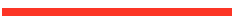
\includegraphics[width=0.1\textwidth]{sepLine}
         \vspace{0.6cm}
         \vfill
\end{titlepage}

	
	\tableofcontents
	\begingroup
\let\clearpage\relax
	\listoffigures
\endgroup

	\chapter{Introduction}
	{
		\section{Motivations}
		{
			\paragraph{} When it comes to learning real-world manipulation tasks (grasping an object, catching a ball, etc) common machine learning algorithms are sometimes unable to come up with feasible solutions, or at least fail to do so in an acceptable computational time. This is mostly due to the size of the action-state space which has to be explored, exponentially growing with the dimensionality of a given problem.  A natural way to accelerate the learning process is to provide a learning algorithm with prior beliefs on its environment, as well as demonstrations of the task.
			
			\paragraph{} Such prior beliefs are often achieved thanks to demonstrations (assumed to be near optimal) performed by a human teacher. Even though this approach is covered in the literature (see \ref{subsection::lfd}), it is not really clear how to learn from a suboptimal teacher, regardless of its level of sub-optimality. Such learning abilities could enlarge the human - robot interactions possibilities, as only little knowledge in robotics or artificial intelligence would be needed to help a robot learn a task. 
			
			\paragraph{} We call a teacher suboptimal if it provides imperfect demonstrations of a task. A demonstration can be imperfect in many ways. For instance, it could poorly transfer to the robot abilities, or simply be a naive way of completing the considered task (in the sense that it does not optimize a numerical criterion evaluating the fitness of an agent's behavior). Also, we will use the term \emph{largely suboptimal} for teachers providing demonstrations that are harmful for the learner or present obvious drawbacks at completing a task. 
			
			\paragraph{} Throughout this semester project, we wanted to gather some intuition on how to learn from (largely) suboptimal teachers. The following examples motivate the approach we decided to follow. 
			
			\subsection{Motivating examples}
			\paragraph{} Let's consider the example of a robotic arm learning to grasp an object: an unexperienced teacher might provide demonstrations that operate near the robot's workspace limits (which is often undesirable in robotics). Even if the robotic arm should not trust this demonstration if it wants to learn an optimal solution, it would be unwise to simply discard it since it contains important information relative to the task (pose of the object, joint coordination, etc). We must therefore find a way to exploit such demonstrations in order to extract relevant information without falling into its suboptimal reproduction. 
			
			\paragraph{}We can rephrase the previous problem by considering the case of a child learning to dance (or any other technical skill). Because the dance teacher does not have the same physical abilities as the child, she/he might give her/him a suboptimal way (with respect to the child's physical abilities) of performing dance moves. In a ideal learning process, the child would use the prior information given by the teacher to practice. She/he will soon be aware of her/his own abilities, and can then start learning by herself/himself, exploring around what she/he has learnt so far. She/he might find that, by slightly changing how he performs some moves, she/he is able to dance better than by blindly listening to the teacher. Therefore, the learning child will first be \emph{compliant} with the teacher, before trying things out by herself/himself once it has become skilled at performing the learned task. 
			
			\subsection{Goal}
			\paragraph{} This semester project aims at introducing a theoretical formulation of this compliance-based behavior, and experimentally test its performance on simple problems.
			
			\paragraph{} The underlying goal behind this objective is to get better intuition about how interactive learning between humans and robots can be achieved. Indeed, we would like to be able to teach a robot from demonstration not only by providing it a large number of trajectories that it will then use as a motion generator, but through interaction. This can be done by showing a robotic arm, at different times of its learning procedure, concrete examples of possible solutions. 
			
			\paragraph{} This approach also allows us to tackle a somehow different but related problem. Indeed, the teacher might not be a human but another learner, only better trained than the current learner. In such a case, we would like the learner to quickly find if it can trust its mentor, and if not where it should focus its computations to overcome its mentor's sub-optimality. Such questions will therefore be tackled in this report. 
		}
		\section{Learning from Demonstration}
		{	
			\label{subsection::lfd}
			\paragraph{} The process of mapping states to actions (also called \emph{policy}) is crucial for many robotics applications. The development of policies by hand is particularly challenging for real-world tasks, and requires a fairly advanced level of expertise. This is why machine learning techniques have been applied to derive policies.
			
			\paragraph{} Learning from demonstration (LfD) is a framework where a robot can learn a policy from interacting with a human. It particularly focuses on the cases where a mentor provides demonstrations on how to perform a task. LfD mostly lies on the principle that the learning robot can be taught new tasks by end-users, without having to be programmed again. Such robots must therefore be able to generalize from demonstration, namely to infer the task the teacher is demonstrating. Therefore, LfD shows great promises for a global use of robotics systems outside of expert communities. Another main advantage of LfD is to focus the dataset in areas that actually matter for a given task or problem. 
			
			\paragraph{} Learning from demonstration is still a hot research topic, and gives rise to different technical and theoretical issues. A complete introduction to this subject can be found in \cite{Billard2016}.  One common approach is to draw inferences for a policy - thanks to statistical learning tools - from the teacher's demonstrations (that are therefore used in a supervised learning way to learn a motion generator). This technique is known as \emph{behavior cloning} or the \emph{mapping function} approach (see \cite{argall2009survey}), and was successfully used for many applications (see \cite{hovland1996skill} and \cite{mataric2002} for examples). However, this method is applicable only if the reproduction of the task by a learner operates in a somehow similar context as in when the demonstrations were performed. Hence, the task might need to be re-learned when the environment slightly changes. This last remark is one of the main argument for the use of reinforcement learning based methods for learning from demonstrations. Indeed, in this framework, an agent could discover new control policies by itself, while getting help from the initial demonstrations. 
			
			\paragraph{} The use of reinforcement learning in the context of learning from demonstrations has been studied under many different aspects, and is still an active research field.  A natural way to use demonstrations in a reinforcement learning approach is to use them as \emph{bootstrap} for a reinforcement learner (see \cite{Billard2016}). For instance, one can use the teacher's policy as a roll-out to get an initial estimate of the value of different teacher actions. The approach that we are more interested in involves using demonstration at exploration time. For instance, one could decide to let the demonstrator take over during one trial, or even create mixtures of policies involving the teacher's one in a policy search context (see \cite{ross2011reduction}). In a exploration-exploitation tradeoff context, the idea of using a policy guided by the teacher was also used in \cite{chu2017analyzing}. The idea followed in this report somehow relates to the last two ones, but enables to have adaptive mixtures / exploratory policies. 
			
			\paragraph{} Another approach to LfD was recently developed in the framework of \emph{Inverse Reinforcement Learning} (IRL). The main justification of this approach comes from the fact that engineering a well-behaved reward function quickly becomes intractable for complex tasks. The idea of IRL (at least in a LfD context) is therefore to consider the demonstrations as expert moves, and learn the reward function that will best explain the observed (allegedly optimal) policy. This approach have some inherent ambiguities that were recently partially or completely solved (see \cite{abbeel2004apprenticeship} and \cite{ziebart2008maximum}). A formal gap between LfD and IRL was also drawn in \cite{piot2017}. One of the main disadvantages of IRL for our concerns is that demonstrations are considered as expert moves - excluding therefore suboptimal teachers. The consideration of such teachers was also recently studied in a Bayesian framework (see \cite{choi2015hierarchical}).
			
		\paragraph{} As stated earlier, most of the existing approach in LfD rely on the hypothesis that the dataset contains some high-rewarding demonstrations. With a compliant-based exploration approach, we hope to loosen that assumption and teach a reinforcement learner from (largely) suboptimal demonstrations. 
				
		}
		\section{Outline}
		{
			
			\paragraph{} To grasp ideas and intuitions about a compliant-based imitation learning method, we are going to start with a fairly simple environment and an explicit task. A simple enough state space will allow us to better understand how compliance in learning by demonstration could be used with a reinforcement learning formulation. We expect to be able to generalize to more complex situations once the understanding on a simple but generic model is mastered. 
			
			\paragraph{} Hence, after defining a simple two dimensional grid-world state space with a simple action set, we will quickly study how well different classical reinforcement learning algorithms performs on such a space. We will then introduce new exploration policies, where the learner - beside searching for the optimal policy - evaluates the optimality of its teacher. We will also focus on the relation between the learner and the prior information that its mentor's recommandations represent. Especially, we will study how well a learner can overcome its mentor sub-optimality, focusing on largely suboptimal mentors. 
		}
	}
	\newpage
	
	\chapter{Reinforcement Learning}
	{
		\paragraph{} The reinforcement learning approach being an essential aspect of this project, this chapter is intended to review the foundations of the reinforcement learning theory and its practical implementations. 
		\section{Formulation}
		{
			\subsection{Definitions}
			{
				\paragraph{} Reinforcement learning is a framework in which an \emph{agent} (or a \emph{learner}) learns its actions from interaction with its environment. The environment generates scalar values called \emph{rewards}, that the agent is seeking to maximize over time. 
			
				\paragraph{} Let $\mathcal{S}$ denote the state space in which our agent evolves (the localization of a robot on a grid for instance), and $\forall{s}\in\mathcal{S}$ we will define the action state $\mathcal{A}(s)$, describing all possible action that can be taken by the agent at state $s$. When taking an action from a state $s_t$, the agent finds itself in a new state $s_{t+1}$ where it receives a reward $r_{t+1}\in\mathbb{R}$. The action taken is sampled over a probability distribution from the joint space of state and action: 
				\begin{equation}
					\begin{aligned}
						\pi \,  : \, \mathcal{S}\times\mathcal{A}(s) \, &\to [0,1]\\
							 (s,a) \, &\to \,  \pi(s,a)
					\end{aligned}
				\end{equation}	
				where $\pi(s,a)$ is the probability of picking action $a$ in state $s$. Such a distribution is called the agent's \emph{policy}. The key goal of reinforcement learning is teaching an agent on how to change its policy to maximize its reward on the long run. 
				
				\paragraph{} The agent indeed seeks to maximize the \emph{expected return} $R_t$ mapping the reward sequence into $\mathbb{R}$. A commonly used expression for this value employs a \emph{discount factor} $\gamma \in [0,1]$, allowing to make the agent's more sensible to rewards it will get in a close future: 
				\begin{equation}
					R_t = \sum_{i=0}^T \gamma^i r_{t+1+i}
				\end{equation}
				This also allows to adapt this formulation to continuous tasks, where there are no terminal states and the task goes on indefinitely (there are no \emph{episodes} in the learning). 
			}
			\subsection{Markov decision process}
			{
				\paragraph{} To make the problem tractable, we ask for the state signal to comply with Markov's property, hence to be \emph{memory-less}. For instance, we want to be able to write that, in a stochastic environment, $\forall s'\in\mathcal{S}$: 
				\begin{equation}
					\mathbb{P}\left( s_{t+1}=s' \, \vert \, a_t, s_t, \hdots, a_1,s_1\right) = \mathbb{P}\left( s_{t+1}=s' \, \vert \, s_t, a_t\right)
				\end{equation}
				
				\paragraph{} Hence, every reinforcement learning problem can be represented by a \emph{Markov Decision Process}, that consists in a 5-tuple $\left(\mathcal{S}, \mathcal{A}, \mathcal{P}_{\cdot}(\cdot,\cdot), \mathcal{R}_{\cdot}(\cdot), \gamma \right)$ where: 
				\begin{itemize}[label=$\triangleright$]
					\item $\mathcal{S}$ is the agent's state space
					\item $\mathcal{A}$ is the agent's action space
					\item $\forall s,s'\in\mathcal{S}, \, \forall a\in\mathcal{A}(s)$,  $\mathcal{P}_a(s,s') = \mathbb{P}(s_{t+1}=s'\, \vert \, s_t = s, a_t = a)$ is the probability that action $a$ in state $s$ will lead the agent to transitioning to state $s'$.
					\item $\forall s,s'\in\mathcal{S}, \, \forall a\in\mathcal{A}(s)$,  $\mathcal{R}_a(s,s')$ is the immediate reward perceived by the agent when transitioning from state $s$ to $s'$ when taking action $a$. 
					\item $\gamma$ is the discount factor. 
				\end{itemize}
				
				\paragraph{} A \emph{finite Markov decision process} designates a MDP for which both the action and state space are finite. 
			}
			\subsection{State and action value function}
			{
				\paragraph{} Most of the reinforcement learning algorithms are based on value function evaluation. A value function is a function mapping the state space in $\mathbb{R}$, estimating how good (in terms of expected future reward) it is for the agent to be in a given space. More precisely, a value function $V^\pi(\cdot)$ evaluates the expected return of a state when following the policy $\pi$. $V^\pi(\cdot)$ is called the \textbf{state-value function}. 
				\begin{equation}
					\forall{s}\in\mathcal{S}, \quad V^\pi(s) = \E[\pi]{R_t \, \vert \, s_t = s}
				\end{equation}
				The \textbf{action-value function} evaluates the value of taking a given action, and then following the policy $\pi$: 
				\begin{equation}
					\forall{s,a}\in\mathcal{S}\times\mathcal{A}(s), \quad Q^\pi(s,a) = \E[\pi]{ R_t \, \vert \, s_t=s, \, a_t=a}
				\end{equation}
				
				\paragraph{} Both those functions satisfy particular recursive relationships known as the \emph{Bellman equations}. It is shown that (see \cite{Sutton98a}) we have the following results: 
				\vspace{10pt}
				
				\coolbox{white}{\textcolor{black}{Bellman equations for Markov Decision Process}}
				{
					\begin{itemize}[label=$\triangleright$]
						\item Bellman equation for the state-value function: $\forall s \in\mathcal{S}$ 
						\begin{equation}
							V^\pi(s) = \sum_{a\in\mathcal{A}}\pi(s,a)\sum_{s'} \mathcal{P}_a(s,s')\left[\mathcal{R}_a(s,s') + \gamma V^\pi(s')\right]
						\end{equation}
						\item Bellman equation for the action value function: $\forall{s,a}\in\mathcal{S}\times\mathcal{A}(s)$: 
						\begin{equation}
							Q^\pi(s,a) = \sum_{s'}\mathcal{P}_a(s,s')\left[ \mathcal{R}_a(s,s') + \gamma V^\pi(s')\right]
						\end{equation}
					\end{itemize}
				}
			}
			\subsection{Optimal policies}
			{
				\paragraph{} The value functions define a partial ordering in the policy space. A policy $\pi$ is therefore said to be better than $\pi'$ (or $\pi\geq \pi'$) if $\forall{s}\in\mathcal{S}$, $V^\pi(s) \geq V^\pi(s')$. We are looking for $\pi^*$ so that: 
				\begin{equation}
					\forall\pi, \quad \pi^* \geq \pi 
				\end{equation}
				
				It was showed that for finite MDPs, there is always at least one policy that is better our equal to all others, and therefore is called the \emph{optimal policy} $\pi^*$. As shown in \cite{Sutton98a}, the state-value and action-value function verify the \emph{Bellman optimality equations}. 
				
				\vspace{10pt}
				
								\coolbox{white}{\textcolor{black}{Bellman optimality equations}}
				{
					\begin{itemize}[label=$\triangleright$]
						\item Bellman optimality equation for the state-value function: $\forall s \in\mathcal{S}$ 
						\begin{equation}
							V^\pi(s) = \max_{a\in\mathcal{A}(s)}\pi(s,a)\sum_{s'} \mathcal{P}_a(s,s')\left[\mathcal{R}_a(s,s') + \gamma V^\pi(s')\right]
						\end{equation}
						\item Bellman optimality equation for the action value function: $\forall{s,a}\in\mathcal{S}\times\mathcal{A}(s)$: 
						\begin{equation}
							Q^\pi(s,a) = \sum_{s'}\mathcal{P}_a(s,s')\left[ \mathcal{R}_a(s,s') + \max_{a\in\mathcal{A}(s')} Q(s',a') \right]
						\end{equation}
					\end{itemize}
				}
				
				\paragraph{} Those relations are essential in understanding the solving algorithms that will be presented later. 
			}
		}


			\paragraph{} There exists several ways of solving (i.e computing the optimal policy) a Markov Decision Process, that can generically be separated in two categories: \emph{model-based} and \emph{model-free} methods. 
		\section{Dynamic Programing}
		{
			\paragraph{} Dynamic programing is a mathematically well-developed theory. It requires the complete and accurate model of the environment, making it a model-based method. 
			
			\paragraph{} Dynamic programing methods aims at computing the optimal value function at every state of state space. This could, of course, be done by solving the $\vert \mathcal{S} \vert $ equations of $\vert \mathcal{S} \vert $ unknowns that are the Bellman equations for a given policy, and then evolve that policy toward a better one, based on the current value function. Of course, this approach is computationally intractable for large state space and therefore needs to be adapted. Nonetheless, it gives a first approach of the idea behind dynamic programing. 
				
			\subsection{Generalized policy iteration}
			{
				\paragraph{} The generalized policy iteration methods rely on alternating two processes known as \textcolor{red}{policy evaluation} and \textcolor{red}{policy improvement}. 
				\begin{itemize}[label=$\triangleright$]
					\item Policy evaluation deals with estimating the value function of a given policy $\pi$, without directly solving the full system given by Bellman equations. The idea is actually pretty simple: use Bellman's equation as an update rule, the value function being a fixed point. After setting the tabled value function to an initial value, the algorithm iterates by performing what is called \emph{full Bellman backups}: 
					\begin{equation}
						\forall{s}\in\mathcal{S}, \quad V_{k+1}^\pi(s) = \sum_{a\in\mathcal{S}} \pi(s,a)\sum_{s'}\mathcal{P}_a(s,s') \left[\mathcal{R}_a(s,s')+V_k^\pi(s')\right]
					\end{equation}
					This algorithm converges under the same assumptions that guarantee the existence of the value function, and has the generic name of \emph{iterative policy evaluation}. They are many refining for speeding up that process (reduced backups, prioritized sweeping) which we won't address here. 
				\item Policy improvement is a process that from a given policy value function, returns a better or equal policy compared to the latter. The simplest way to do that is to consider, for every state $s\in\mathcal{S}$, every action-value functions: 
				\begin{equation}
					Q(s,a) = \sum_{s'}\mathcal{P}_a(s,s')\left[\mathcal{R}_a(s,s') + \gamma V\pi(s')\right], \quad a\in\mathcal{A}(s)
				\end{equation}
				and then to build $\pi'$ to be \emph{greedy} with respect to those actions-values: 
				\begin{equation}
					\pi'(s) = \argmax{a\in\mathcal{A}(s)}{Q(s,a)}
				\end{equation}
					The policy improvement theorems then ensures that $\pi'\geq \pi$. 
				\end{itemize}
				
				\paragraph{} Hence, generalized policy improvement are a set of methods that iteratively combine those two sub-methods to compute the optimal policy for a given MDP. Of course, one does not have to perform all sweeps of value evaluation before improving the policy to converge toward an optima (indeed, many times our sweeps won't have any affect on the greedy policy). They are many ways to combine the two (prioritized sweeping, asynchronous dynamic programing), but the most used and one of the most quickest way to converge is to use the value iteration algorithm. 
			}	
			\subsection{The value iteration algorithm}
			{
				\paragraph{} The value iteration algorithm takes the limit of the behavior we just described, and stops the value evaluation procedure after only \emph{one state space sweep}. It therefore performs a simple backup procedure: 
					\begin{equation}
						\forall{s}\in\mathcal{S}, \quad V_{k+1}(s)  = \max_{a\in\mathcal{A}}  \sum_{s'}\mathcal{P}_a(s,s')\left[\mathcal{R}_a(s,s') + \gamma V_k^\pi(s')\right]
					\end{equation}
					For any arbitrary $V_0$, it is shown that $V_k\to V^*$ as $k\to\infty$, under the same hypothesis that ensure the existence of the optimal value function $V^*$. As one can notice, it actually implements the \emph{Bellman optimality conditions} as an update rule !
				}
			}
		
		
		\section{Temporal differences methods}
		{
			\paragraph{} Temporal difference methods can be seen as a combination of dynamic programing and another kind of learning called Monte Carlo methods, where the expected return are approximated via sampling. Like dynamic programming, TD methods are said to bootstrap (meaning that they build their estimators through already estimated values), but are \emph{model-free} methods and learn from experience. 
			
			\paragraph{} The justification, proof of convergences and literature and those models is pretty wide, hence we will not cover them in this report. However, a full description of those methods can be found in \cite{Sutton98a}. 
			
			\subsection{On-policy method: SARSA}
			{
				\paragraph{} The SARSA algorithm is an \emph{on-policy} control method, meaning that the algorithm updates the value function and improves the current policy it is following. At state $s_t$, it chooses an action $a_t$ from its policy and follows it. After observing the reward $r_{t+1}$ and the next state $s_{t+1}$, it again chooses an action $a_{t+1}$ using a soft policy and performs a one-step backup: 
				\begin{equation}
					Q(s_t,a_t) \leftarrow Q(s_t,a_t) + \alpha\left[r_{t+1} + \gamma Q(s_{t+1},a_{t+1}) - Q(s_t,a_t)\right]
				\end{equation}
				It therefore relies on a 5-tuple $(s_t,a_t,r_{t+1},s_{t+1},a_{t+1})$ to perform the udpate, giving it the State Action Reward State Action (SARSA) name. 
				\vspace{10pt}
				
				\coolbox{white}{\textcolor{blue}{The General Sarsa Algorithm}}
					{
						\begin{algorithm}[H]
	 					\SetAlgoLined
						\LinesNumbered
						\emph{\textsf{1. Initialize}} $Q(s,a)$ arbitrarily $\forall (s,a)\in\mathcal{S}\times\mathcal{A}(s)$ \\
						\BlankLine
						\BlankLine
						\emph{\textsf{2. Repeat}} for each episode: \\
						\Indp \Indp 
							Initialize $s$ \\
							Choose $a\in\mathcal{A}(s)$ using a soft policy derived from $Q$ (typically $\varepsilon$-greedy) \\
							Repeat for each step of the current episode:   \\
							\Indp \Indp 
								Take $a$, observe $r,s'$ \\
								Choose $a'$ from $s'$ using policy derived from $Q$ 
								$ Q(s,a) \longleftarrow Q(s,a) + \alpha\big[ r + \gamma Q(s',a') - Q(s,a) \big]$ \\
								$a\leftarrow a'$, $s\leftarrow s' $ \\
								
							\Indm \Indm 
						until $s\in\mathcal{S}^+$.
						\Indm \Indm 
						\end{algorithm}
					}
					
					\paragraph{} The convergence properties of SARSA depend on the nature of the policy's dependency on Q. Indeed, SARSA converges with probability 1 to the optimal policy as long as all the sate and actions pairs are visited an infinite number of time, and the policy converges in the limit to the greedy policy. This is done, for instance, by turning the temperate of a softmax based policy to 0, or by having $\eps\to 0$ for a $\eps$-greedy policy. For SARSA to converge, we also as the learning rate to comply with the stochastic approximation conditions: 
					\begin{equation}
						\sum_k \alpha_k(a) = +\infty \quad { and } \quad \sum_k \alpha_k(a)^2 < +\infty
					\end{equation}
					where $\alpha_k(a)$ is the learning rate for the k\textsuperscript{th} visit of the pair $(s,a)$. 
					
			}
			\subsection{Off-policy method: Q-learning}
			{
				\paragraph{} The Q-learning algorithm is an off-policy method who learns to directly approximate $Q^*$, independently of the policy being followed. Its update rule is given by:
				\begin{equation}
					Q(s_t,a_t) \leftarrow Q(s_t,a_t) + \alpha \left[ r_{t+1} + \gamma \max_{a\in\mathcal{A}(s_{t+1})} Q(s_{t+1},a) - Q(s_t,a_t)\right]
				\end{equation}
				The actual policy being followed still has an effect in that it determines which state-actions pairs are visited and updated. However all that is required for convergence it that all pairs continue to be updated. 
				\vspace{10pt}
				
				\coolbox{white}{\textcolor{blue}{Q-Learning Algorithm}}
					{
						\begin{algorithm}[H]
	 					\SetAlgoLined
						\LinesNumbered
						\emph{\textsf{1. Initialize}} $Q(s,a)$ arbitrarily $\forall (s,a)\in\mathcal{S}\times\mathcal{A}(s)$ \\
						\BlankLine
						\BlankLine
						\emph{\textsf{2. Repeat}} for each episode: \\
						\Indp \Indp 
							Initialize $s$ \\
							Repeat for each step of the current episode:   \\
							\Indp \Indp 
								Choose $a\in\mathcal{A}(s)$ using arbitrary policy \\
								Take $a$, observe $r,s'$ \\
								$ Q(s,a) \longleftarrow Q(s,a) + \alpha\big[ r + \gamma \max_{a'\in\mathcal{A}(s')}Q(s',a') - Q(s,a) \big]$ \\
								$s\leftarrow s' $ \\
								
							\Indm \Indm 
						until $s\in\mathcal{S}^+$.
						\Indm \Indm 
						\end{algorithm}
					}
				
				\paragraph{} Along with this hypothesis and a slight variation in the usual stochastic approximation conditions, the learned action value function by Q-learning has been shown to converge to $Q^*$ with probability $1$. 
				
				\paragraph{} In some cases, off-learning policies algorithms (like Q-learning) and on-policy ones (like SARSA) can learn different optimal policies (see \cite{Sutton98a}). This is mainly due to the fact that Q-learning performs update like if it was following a greedy policy - which it is not. That leads it to be less sensitive to a possible behavioral policy failure. 
			}
			\subsection{Eligibility traces}
			{
				\paragraph{} In TD(0) approach (described in the latest section), we update the value function in the direction of the \emph{one-step return}: 
				\begin{equation}
					\Delta V_t(s_t)^{(1)} = \alpha \left[ r_t + \gamma V_t(s_{t+1}) - V_(s-t)\right]
				\end{equation}
				The idea behind eligibility traces is to expand that update rule in order to steer the value fonction towards the \emph{n-step return} (or at least until a terminal state is reached):
				\begin{equation}
					\begin{aligned}
					\Delta V_t(s_t) ^{(n)} &= \alpha \left[ r_t + \gamma r_{t+1} + \hdots + \gamma^{n} V_t(s_{t+n})-V_t(s_t)\right]	\\
									&= \alpha \left[R_t^{(n)} - V_t(s_t)\right]
					\end{aligned}
				\end{equation}
				
				\paragraph{} The backups can not only be done toward any n-step return, but toward any average of such returns, as long as the corresponding weights sum-up to one. In this way, the TD($\lambda$) algorithm can be understood as a particular way of averaging $n$-steps returns. With $\lambda<1$, the resulting backup is known as the \textcolor{red}{\emph{$\lambda$-return}}: 
				\begin{equation}
					R_t^\lambda = (1-\lambda) \sum_{n=1}^\infty \lambda^{n-1}R_t^{(n)}
				\end{equation}
				where the weights are fading with $n$. When the runs are episodic, we can write this return as: 
				\begin{equation}
					R_t^\lambda = (1-\lambda)\sum_{n=1}^{T-t-1} \lambda^{n-}R_t{(n)} + \lambda_{T-t-1}R_t^{(T)}
				\end{equation}
				
				\coolbox{white}{\textcolor{blue}{Sarsa($\lambda$) algorithm}}
					{
						\begin{algorithm}[H]
						\label{sarsalambda}
	 					\SetAlgoLined
						\LinesNumbered
						\emph{\textsf{1. Initialize}} $Q(s,a)$ arbitrarily $\forall (s,a)\in\mathcal{S}\times\mathcal{A}(s)$ \\
						\BlankLine
						\BlankLine
						\emph{\textsf{2. Repeat}} (for each episode): \\
						\Indp \Indp 
							Initialize $s,\, a$ \\
							Repeat for each step of the current episode:   \\
							\Indp \Indp 
								Take action $a$, observe $r, s'$. \\
								Choose $a'\in\mathcal{A}(s')$ using soft policy derived from $Q$\\
								$\delta \longleftarrow r + \gamma Q(s',a') - Q(s,a)$ \\
								$e(s,a) \longleftarrow e(s,a) +1 $\\
								For all $s,a$: \\
								\Indp \Indp 
									$ Q(s,a) \longleftarrow Q(s,a) + \alpha \delta e(s,a) $ \\
									$ e(s,a) \longleftarrow \gamma \lambda e(s,a) $\\
								\Indm \Indm 
								$s\leftarrow s'$, $a\leftarrow a'$\\						
							\Indm \Indm 
						until $s\in\mathcal{S}^+$.\\
						\Indm \Indm 
						\end{algorithm}
					}


				\paragraph{} Such a formulation of eligibility traces is known as the \emph{\textcolor{red}{forward view}} of TD($\lambda$), and shows how eligibility traces build the bridge between TD(0) methods and Monte-Carlo one. It is not implementable as is since it is non-causal. There exist a more mechanistic view, equivalent to the forward view (see \cite{Sutton98a}), known as the \emph{backward-view}. It gives birth to causal version of the TD($\lambda$) method. We give as an example the pseudo-code for the SARSA($\lambda$) algorithm above. Its Q-learning equivalent can be found in \cite{Sutton98a}. In the following, we will use the variant of eligibility traces for Q-learning known as Watkins Q-learning.
			}
		}
	
		\section{Grid-world examples}
		{
			\paragraph{} We hereinafter describe two grid-world state spaces, on which we will apply the learning methods derived in the latest section. Such examples are trivial and are displayed here simply to show convergence and behavior of the different algorithms. 
			
			\paragraph{} We will consider the two following state spaces: 
			\begin{figure}[ht!]
				\begin{minipage}{0.4\linewidth}
					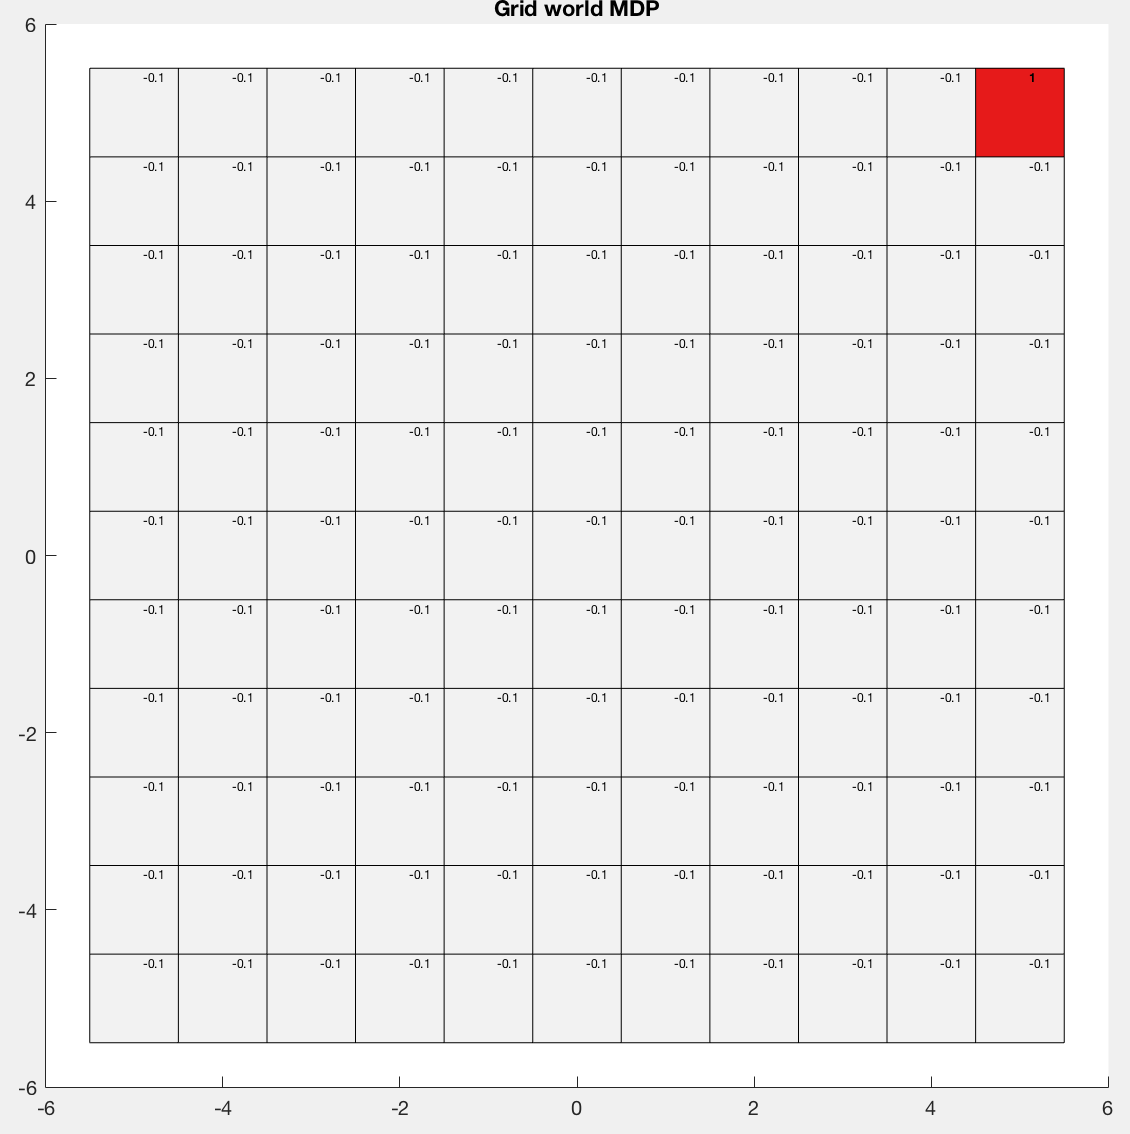
\includegraphics[width=\linewidth]{free_grid}
					\caption{The \emph{free\_grid} state space}
				\end{minipage}
				\hfill
				\begin{minipage}{0.4\linewidth}
					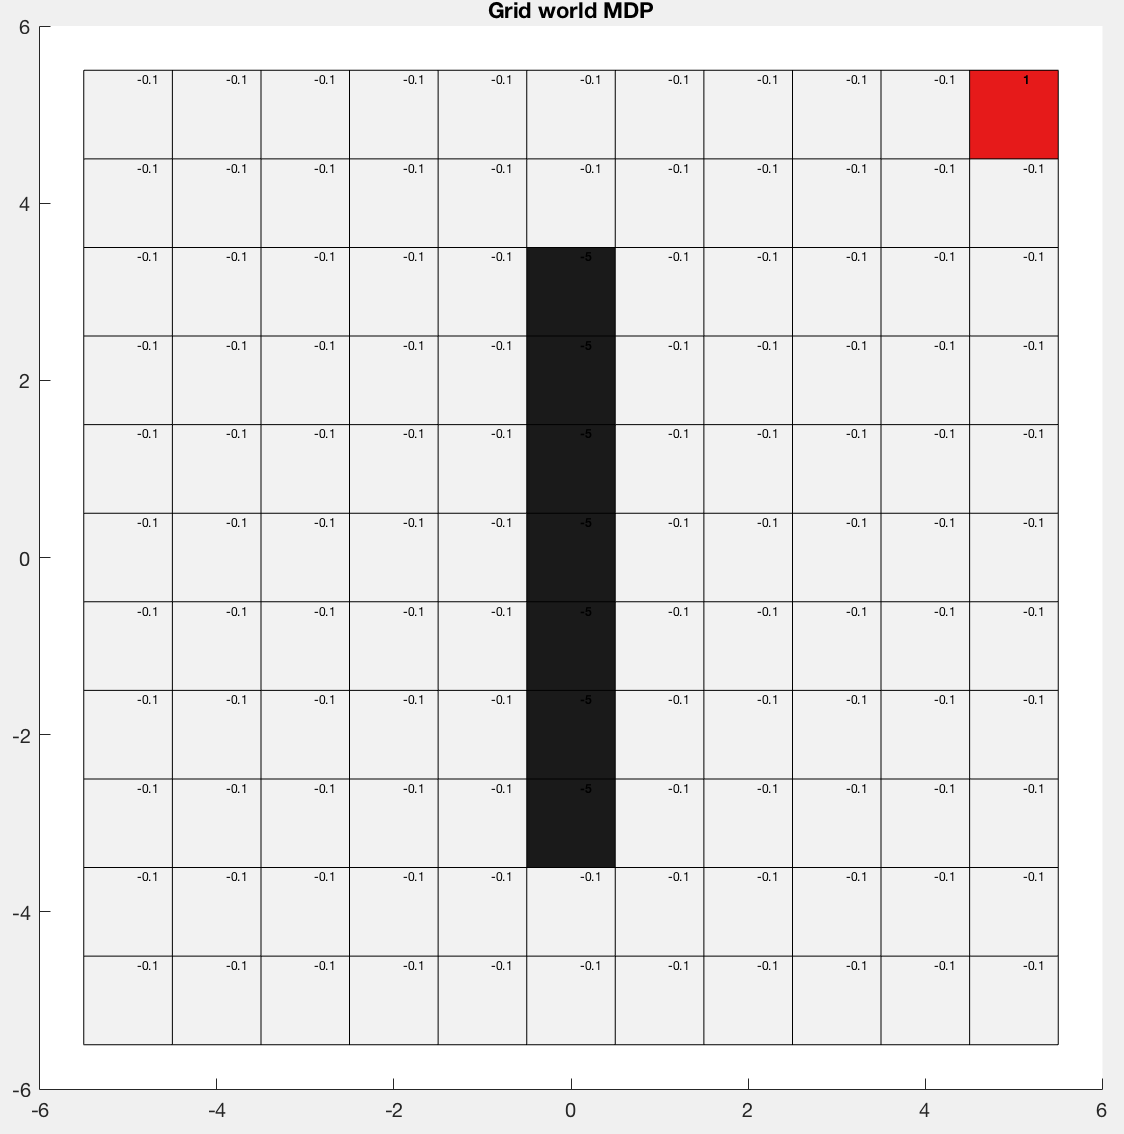
\includegraphics[width=\linewidth]{bar_grid}
					\caption{The \emph{bar\_grid} state space}
				\end{minipage}
			\end{figure}
			\subsection{Dynamic Programing solving}
			{
				\paragraph{} Let us run the DP algorithm on such grid worlds. We will consider a stochastic environnement, with the transition probability: 
				\begin{equation}
					\mathcal{P}_{s,s'}^a = \left\{\begin{aligned} &0.9 &\text{ if }s' = a(s) \\ &0.1 &\text{ otherwise} \end{aligned}\right.
				\end{equation}
				Using a stochastic dynamic, is a first step in designing an environment closer to reality. Also, this allows to provide a simple example (like the one considered) we non-trivial solutions. 
				\paragraph{} Running the value iteration algorithm (assuming we now the environment model), we obtain the following policies and learning curves. The stopping criterion adresses the maximum absolute change brought to the value function as the sweeping goes through the state space: 
				\begin{equation}
					\text{ If } \max_{s\in\mathcal{S}} \vert V_{k+1}(s) - V_k \vert < \delta \text{ then stop}
				\end{equation}
				In practice, $\delta$ is defined to be 0.1\% of the first state-value function update. 
				
				\begin{figure}[ht!]
				\begin{minipage}{0.4\linewidth}
					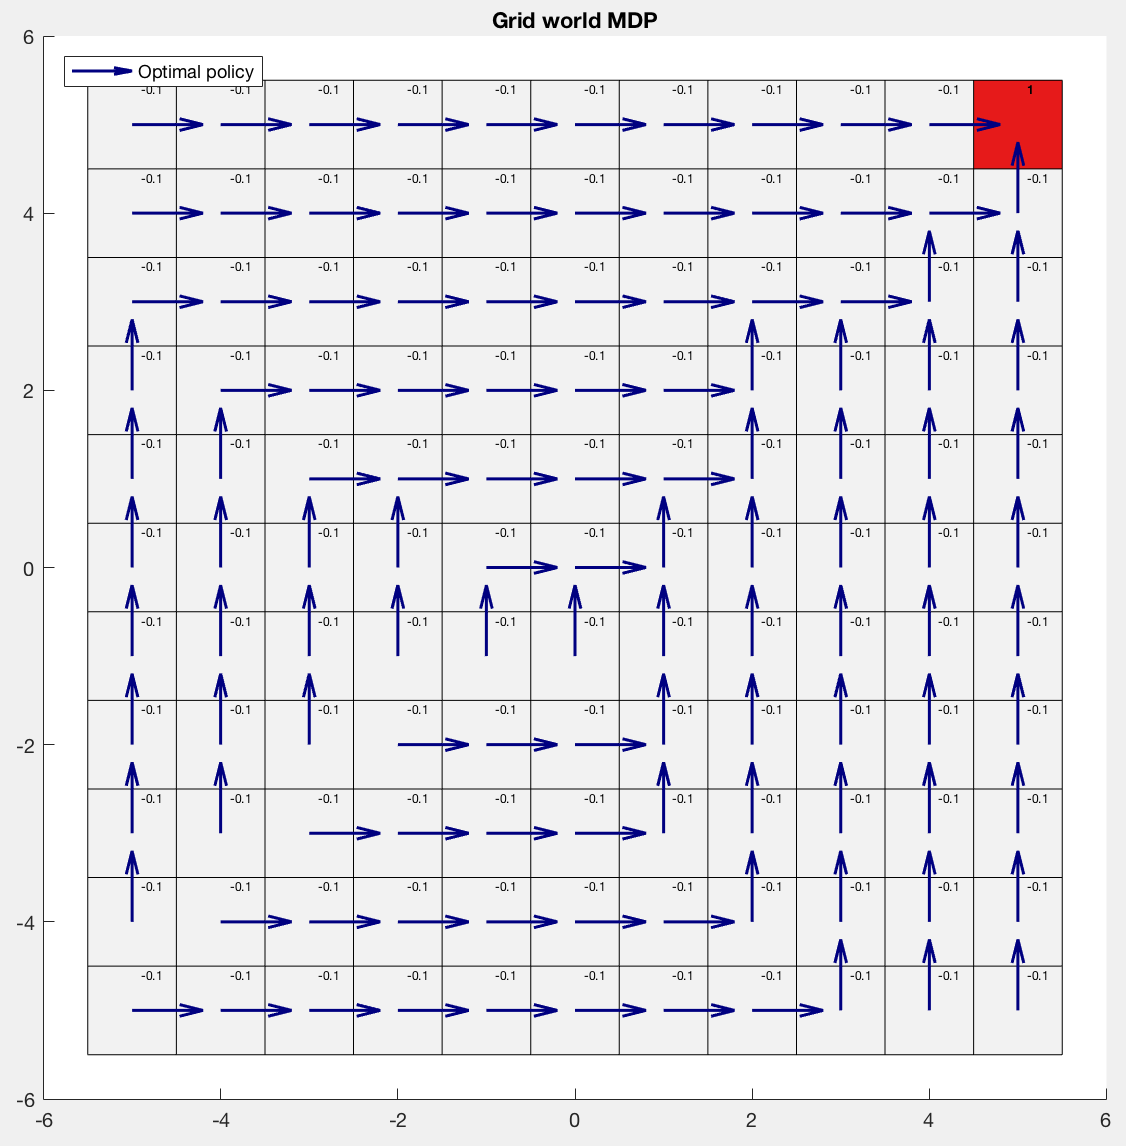
\includegraphics[width=\linewidth]{free_grid_bellman_policy}
					\caption{The \emph{free\_grid} learned optimal policy}
				\end{minipage}
				\hfill
				\begin{minipage}{0.4\linewidth}
					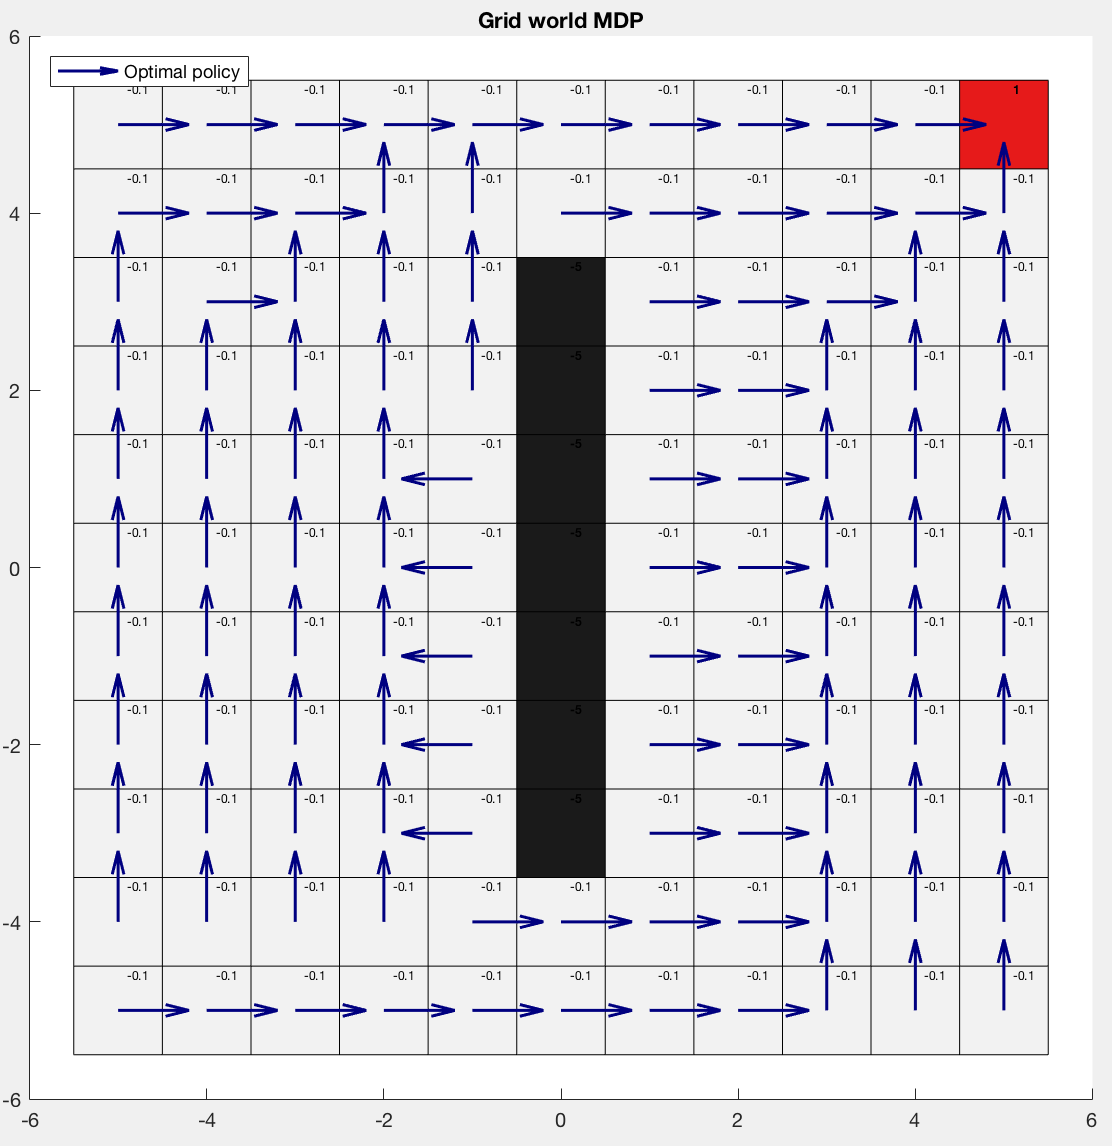
\includegraphics[width=\linewidth]{bar_grid_bellman_policy}
					\caption{The \emph{bar\_grid} learned optimal policy}
				\end{minipage}
				\end{figure}
				
				\begin{figure}[ht!]
				\begin{minipage}{0.4\linewidth}
					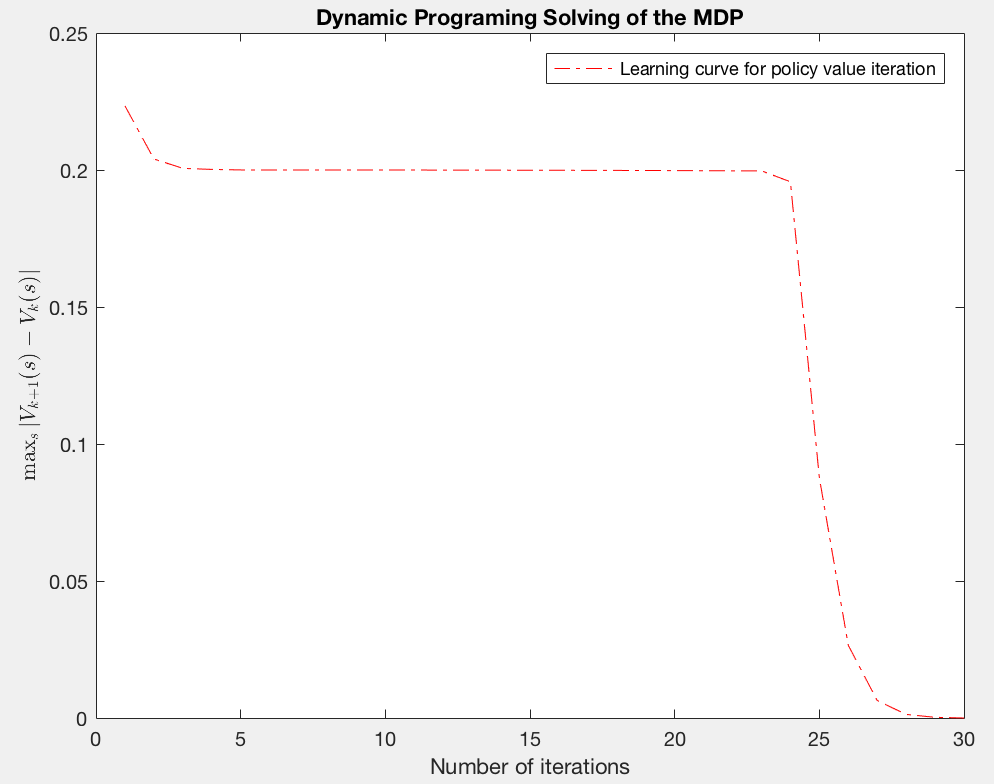
\includegraphics[width=\linewidth]{free_grid_bellman_lc}
					\caption{The \emph{free\_grid} value iteration learning curve}
				\end{minipage}
				\hfill
				\begin{minipage}{0.4\linewidth}
					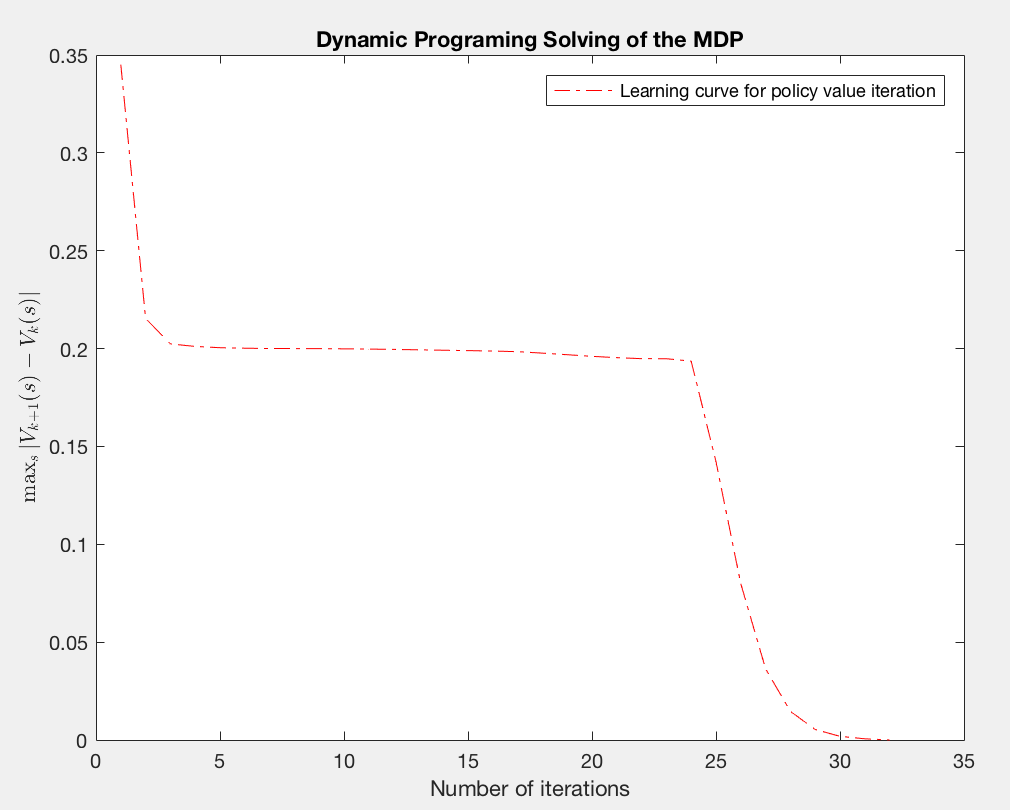
\includegraphics[width=\linewidth]{bar_grid_bellman_lc}
					\caption{The \emph{bar\_grid} value iteration learning curve}
				\end{minipage}
				\end{figure}
				
				\paragraph{} One can notice that for the \emph{bar\_grid} environment, the agent undergoes a longer trajectory than necessary, at the left of the obstacle. This is because of the stochastic nature of the environment, causing the agent to learn to take its distance from the obstacle in order not to accidentally hit it (and then receive a negative reward).The learned policy are indeed optimal, and the next algorithms (SARSA and Q-learning) will try to reproduce them without a model for the environment. 
			}
			\subsection{SARSA solving}
			{
				\paragraph{} We display here the learning curves for the \emph{free\_grid} state space using SARSA. The algorithm manages to learn the optimal policy and the right action-value functions. We use \emph{optimistic initialization} to encourage exploration, and Gibbs sampling for following a soft-policy: $\forall (s,a) \in\mathcal{S}\times \mathcal{A}(s)$ 
				\begin{equation}
					\pi(s,a) = \displaystyle \frac{ e^{Q(s,a)/\tau}}{\sum_{a'\in\mathcal{A}(s)}e^{Q(s,a')/\tau}}
				\end{equation}
				We will tune the distribution's temperature $\tau$ to zero, in order to converge toward the greedy policy w.r.t the learned action-value function. 
				
				\paragraph{} Following this strategy and tuning our learning rate to comply with the stochastic approximation conditions, we obtain the following learning curves. Again, our stopping criterion addresses the \emph{maximum change in the acton-value function over all the trajectories of a mini-batch} (collection of sample trajectories). 
				\begin{figure}[ht!]
					\begin{minipage}{0.4\linewidth}
						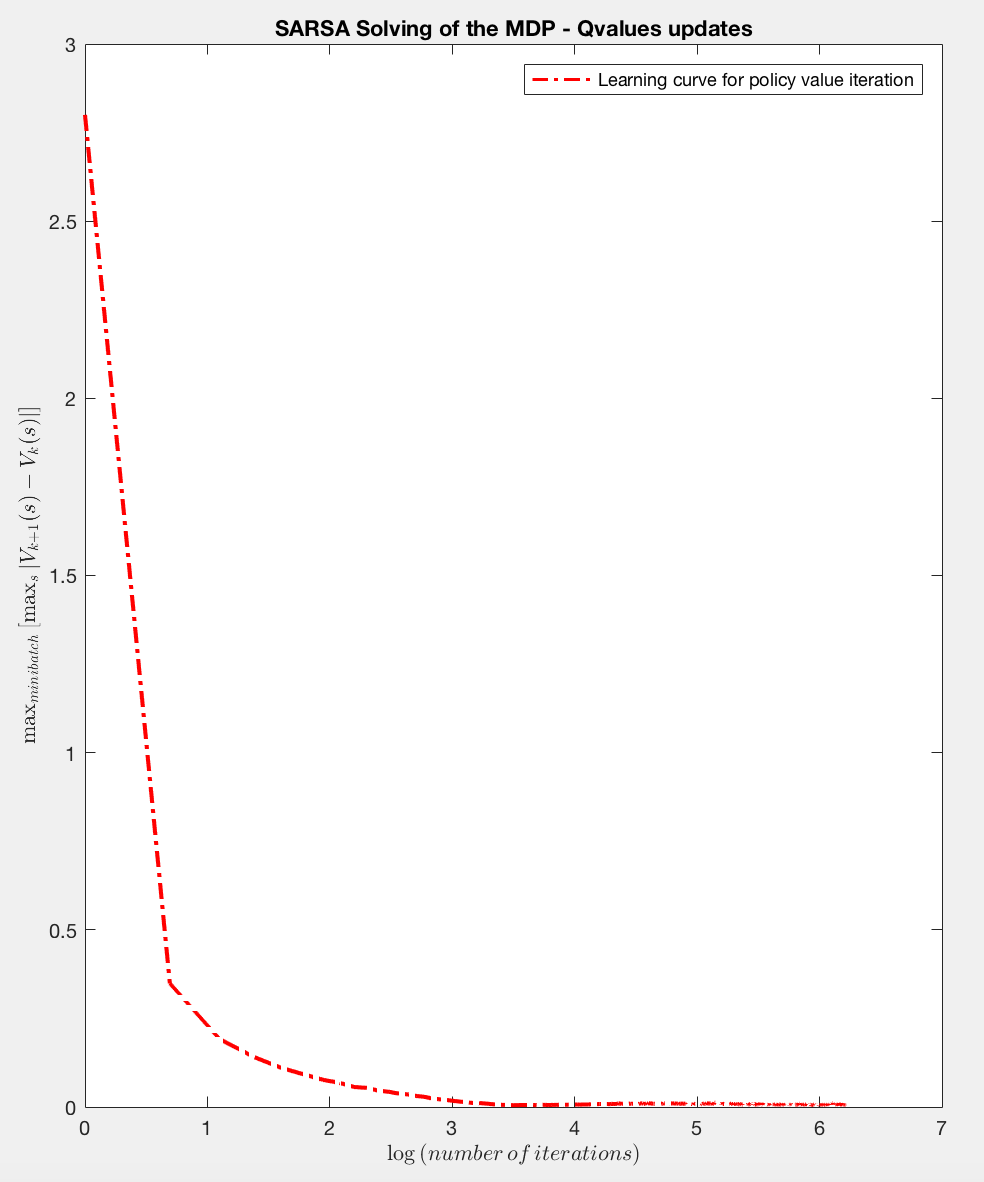
\includegraphics[width=0.9\linewidth]{sarsa_learning_curve_free_grid}
						\caption{Learning curve for SARSA on \emph{free\_grid}}
					\end{minipage}
					\hfill
					\begin{minipage}{0.4\linewidth}
						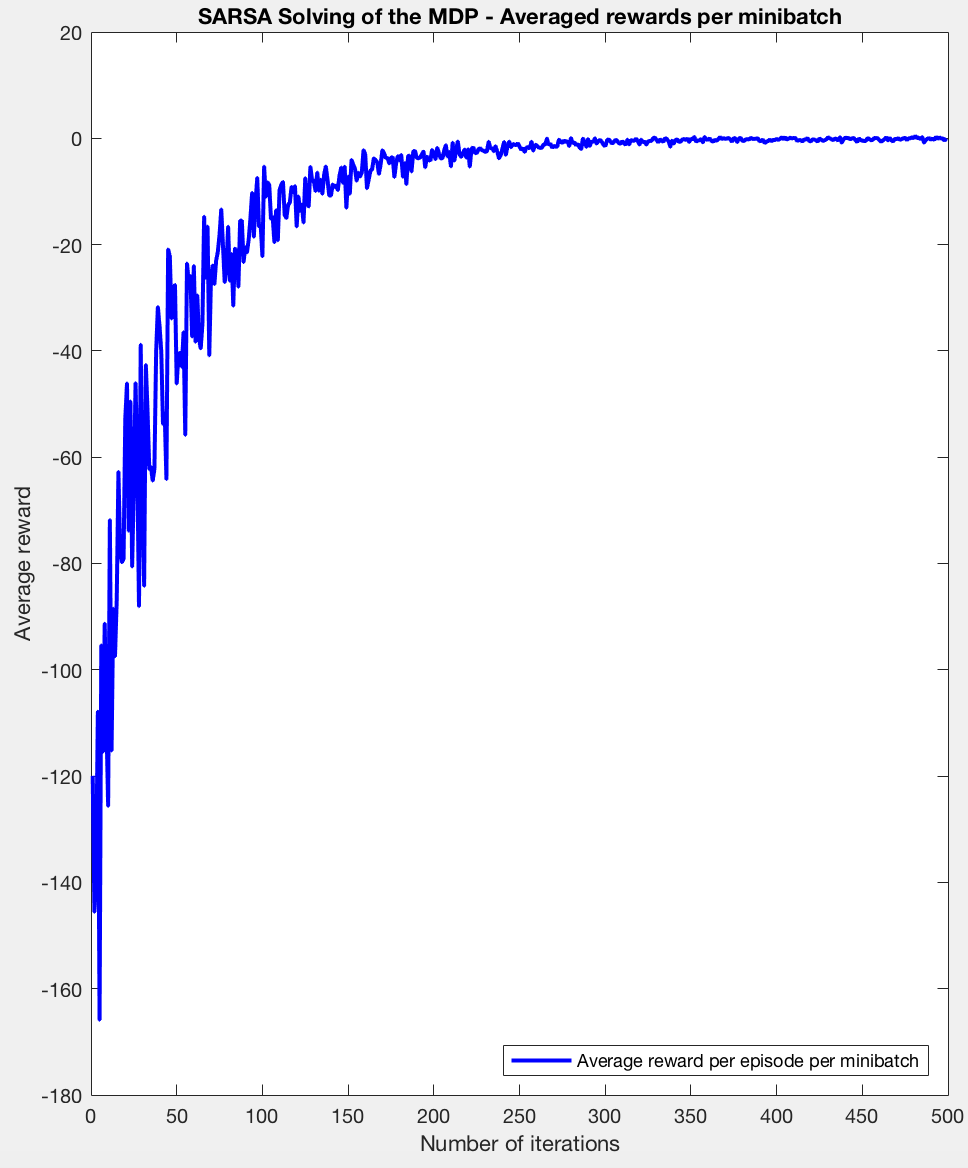
\includegraphics[width=0.9\linewidth]{sarsa_average_rewards_freegrid}
						\caption{Averaged rewards over mini-batch for SARSA on \emph{free\_grid}}
					\end{minipage}
				\end{figure}
				\begin{figure}[h!]
					\begin{minipage}{0.4\linewidth}
						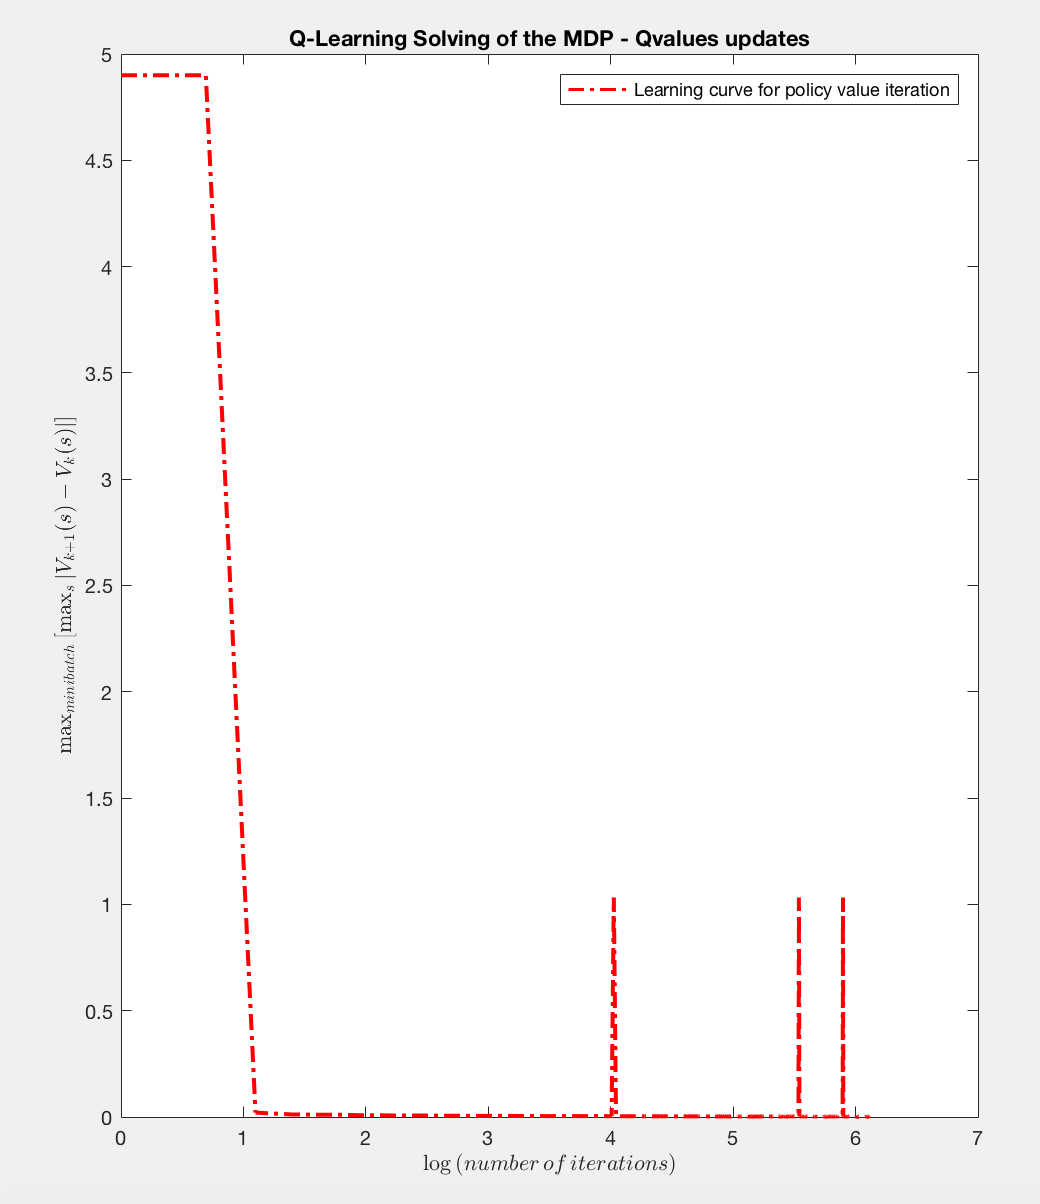
\includegraphics[width=0.9\linewidth]{bargrid_ql_learning_curve}
						\caption{Learning curve for Q-learning on \emph{bar\_grid}}
						\label{fig::bargrid_ql_lc}
					\end{minipage}
					\hfill
					\begin{minipage}{0.4\linewidth}
						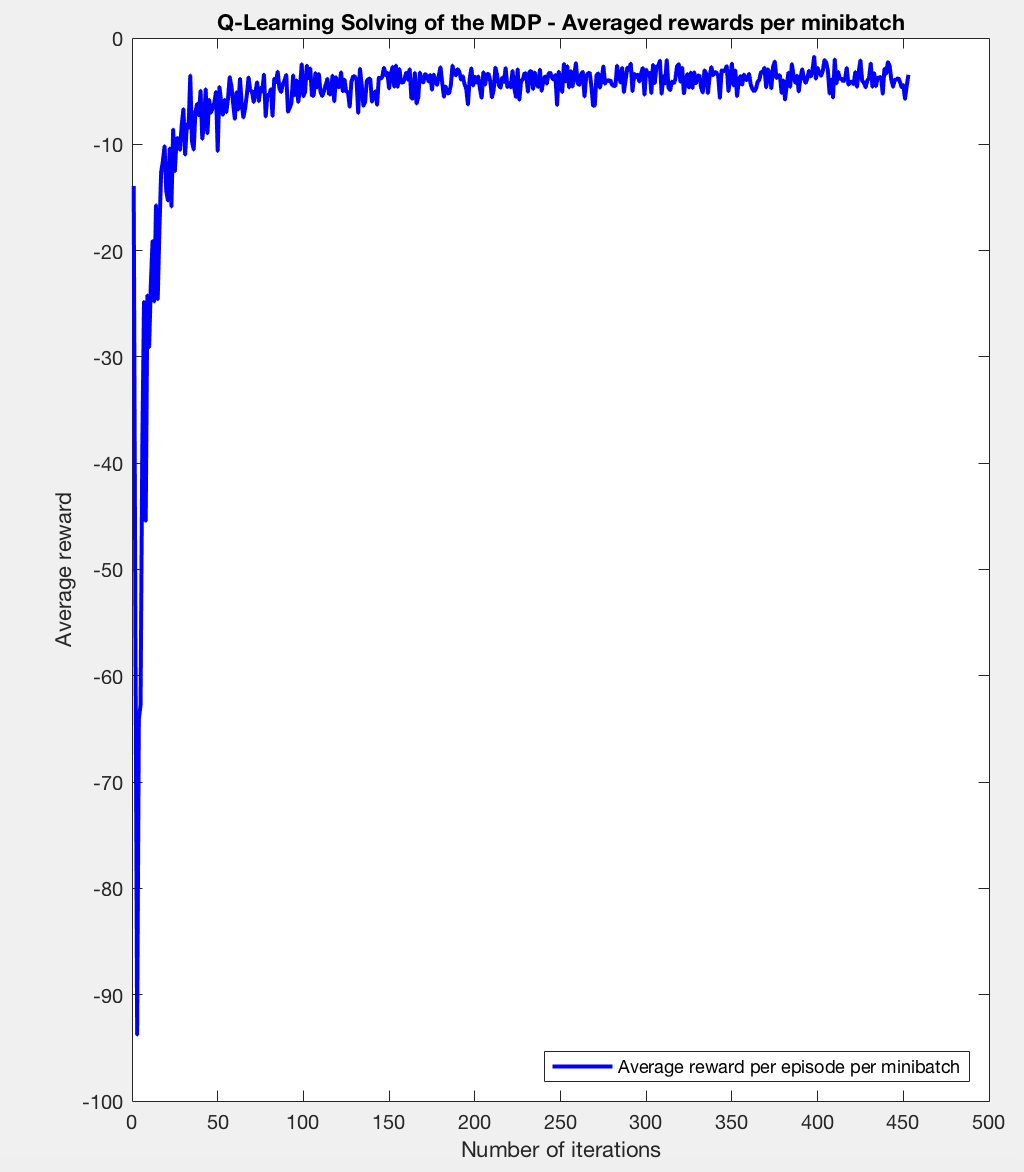
\includegraphics[width=0.9\linewidth]{bargrid_ql_averaged_rewards}
						\caption{Averaged rewards over mini-batch for Q-learning on \emph{bar\_grid}}
						\label{fig::bargrid_ql_ar}
					\end{minipage}
				\end{figure}
				\paragraph{} More precisely, in this example, we use the following dynamics for the temperature and the learning rate: 
				\begin{equation}
					\tau_t = 0.995\cdot\tau_{t-1}
				\end{equation}
				and, $\forall s \in\mathcal{S}, a\in\mathcal{A}(s)$:  
				\begin{equation}
					\alpha_t(s,a) = \frac{\alpha_0(s,a)}{(k(s,a)+1)^{0.55}}
				\end{equation}
				where $k(s,a)$ denotes the number of time the action-state $(s,a)$ was chosen during the learning. Hence, we comply with the greedy-in-limit as well as the stochastic approximation conditions. 
				  
			}
			\subsection{Q-learning solving}
			{
			
				\paragraph{} Figures (\ref{fig::bargrid_ql_lc}) and (\ref{fig::bargrid_ql_ar}) display the learning curves for the \emph{bar\_grid} state space using Q-learning. Again, the algorithm manages to learn the optimal policy and the right action-value functions. We use Gibbs sampling for the behavior policy, without any tuning for the temperature (the behavior policy doesn't need to be greedy in limit). 

			}
		}
	}
	
	\chapter{Compliant Reinforcement Learning}
	\chaptermark{Compliant RL}
	{
		 With our approach, we wish to tackle two topics: on one hand, we wish to develop an imitation based learning framework that \emph{accelerates} the learning process. Also, we wish to apply an adaptive compliance based behavior so that an agent can overcome an arbitrarily suboptimal teacher.
		
		\section{Principle}
		{
			\paragraph{} We start by making a fairly strong hypothesis to simplify our approach. In the following chapters, we will consider that a mentor demonstration provides one recommended action for every state - which is the equivalent of providing one deterministic policy. This somehow out-scopes the case of unique demonstration, but can be understood as a combination of multiple demonstrations.\newline
			Hence, we will consider that a teacher's demonstration is a mapping between the state space $\mathcal{S}$ of the learner and its action set $\mathcal{A}(s)$, $\forall s\in\mathcal{S}$, denoted $\pi_m$: 
			\begin{equation}
				\begin{aligned}
					\pi_m \,:  \, \mathcal{S} &\to \mathcal{A}\\
						     s &\to a_m(s) 
				\end{aligned}
			\end{equation}
			where $a_m(s)$ is the \emph{recommended action} of the mentor at state $s$. 
			\newline 
			Such a hypothesis isn't trivial, and will be discussed later in this report. The main reason it is considered is that it enables to treat the whole state space in the same way - without having to distinguish regions that are provided with demonstrations and regions which are not. 
			
			\paragraph{} As discussed earlier in this report, our goal is to mimic the shifting compliance a child can have with respect to its teacher when learning a new skill. Because this implies making choices as to wether follow a recommended action or sample elsewhere in the action space, it is clear that \textbf{only the action selection should be impacted by the presence of the mentor}. 

			\paragraph{} We will now consider an action selection process based on the teacher's recommandation. We introduce a parameter $p$, that can be understood as a \textbf{confidence measure} in the teacher. The action selection process we chose to follow can be understood as a $p$-greedy action selection with respect to the teacher recommandation and is defined as: 
			\boxedeq{red}
			{
				\forall s\in\mathcal{S}, \quad \pi(s) = \left\{
				\begin{aligned}
					&a_m \, \text{with probability }p \\
					& a \in \mathcal{A}(s)\backslash a_m \text{ with probability } (1-p)
				\end{aligned}\right.
				\label{eq::compliant_exploration}
			}
			The learner therefore has two possibilities: follow the teacher with probability $p$, or take its own action, with probability $(1-p)$. This motivates to call $p$ a confidence measure: the greater $p$ is, the more the learner will trust the teacher and follow its recommandation. In the case where the learner decides to take its own action, it samples in its state space through Gibbs softmax sampling, thanks to its current action-value estimates. \newline
			The updates will follow the SARSA algorithm, and the usual TD(0) updates: $\forall s\in\mathcal{S}, a\in\mathcal{A}(s)$
			\begin{equation}
				Q(s,a) \leftarrow Q(s,a) + \alpha \left[ r + Q(s',a') - Q(s,a) \right]
			\end{equation}
			which are indeed not impacted by the presence of a mentor. Therefore, under the very simple conditions for SARSA to converge to a locally optimal policy (that is, among others, that the exploratory policy is greedy in limit), our algorithms will converge too. 
			
			\paragraph{} The purpose of sections (\ref{section::naive_learners}) and (\ref{section::adaptative_learners}) is to provide the confidence $p$ with different dynamics through time and evaluate the corresponding performances. 
			
		}
		\section{Experimental MDP}
		{
			\paragraph{} To test the effectiveness of the methods we propose, we decided to provide a model that would stay fixed all along the experiments. We will use it in order to compare our different algorithms.
			
			\paragraph{} We designed the state space displayed in figure (\ref{fig::maze_display}). In this environment, all black cells are obstacles. They give out highly negative rewards ($r=-10$). Whenever an agent take the action to enter such a cell, it immediately perceives the negative reward but stays in its current cell. The only positive reward is at the middle of the grid ($r=10$), the only terminal state. Any episode starts at one of the corner of the grid (green cells), and every step spent on a non-terminal cell gives out a small negative reward ($r=-0.1$). The transitions are stochastic, with the transition probability model: 
			\begin{equation}
				s' = \left\{ 
					\begin{aligned}
						&a(s) \text{ with proba } 0.95 \\
						&s'' \neq a(s) \text{ otherwise, uniformly sampled}
					\end{aligned}\right.
			\end{equation}
			 
			 \paragraph{} This state space is big enough for the usual algorithms to learn rather slowly, even if they are greatly enhanced by the use of eligibility traces. Also, all tested algorithms (SARSA, Q-learning, SARSA($\lambda$) and Watkins Q($\lambda$)), because they do not perform infinite exploitation / exploration moves, renders slightly suboptimal policies. 
			
			\begin{figure}[ht!]
				\begin{minipage}{0.45\linewidth}
					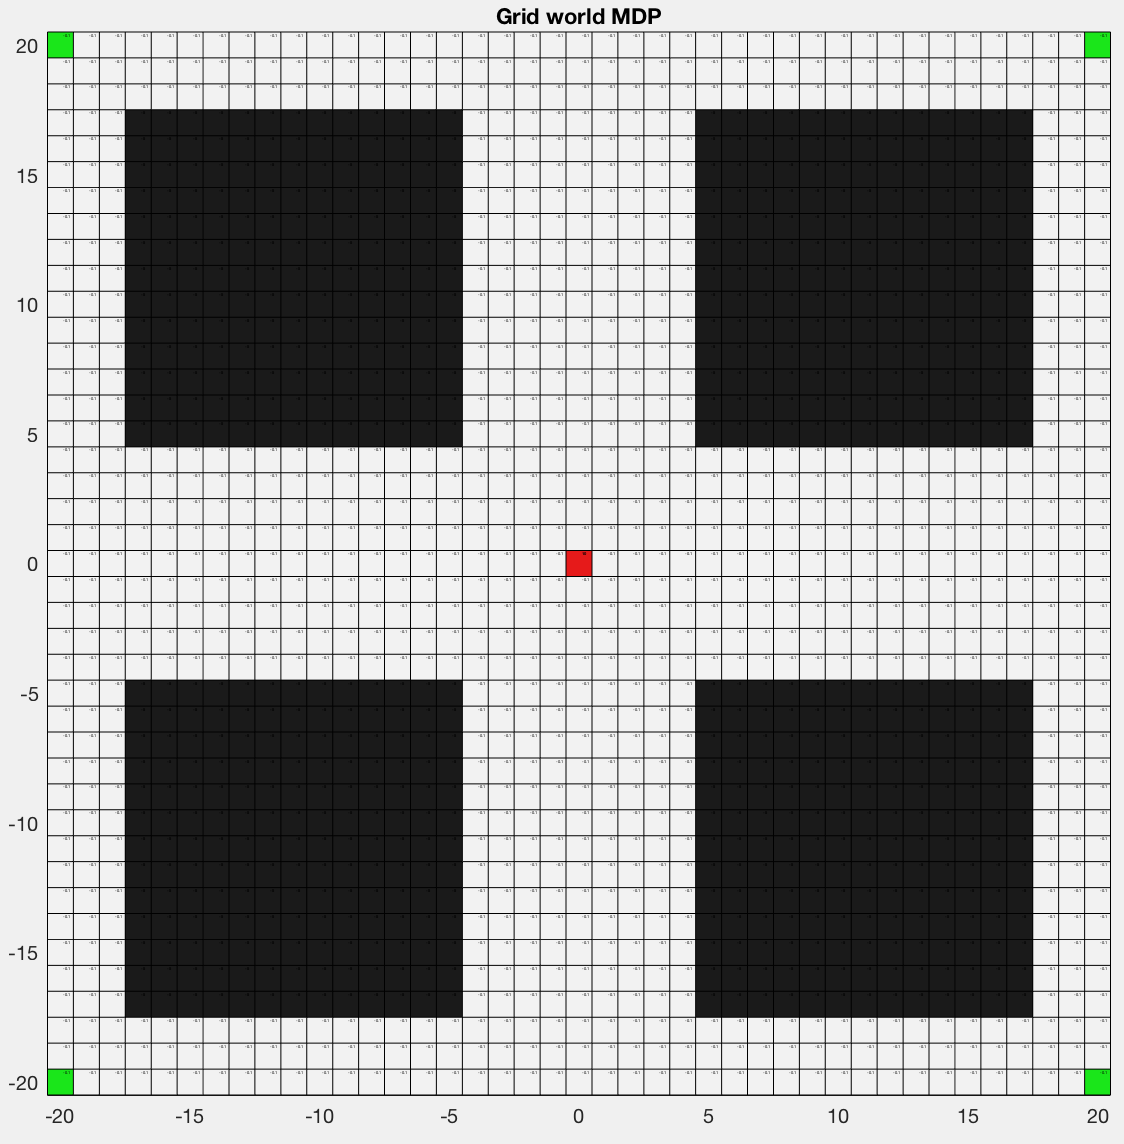
\includegraphics[width=\linewidth]{maze_grid}
					\caption{The \emph{maze\_grid} state space}
					\label{fig::maze_display}
				\end{minipage}
				\hfill
				\begin{minipage}{0.45\linewidth}
					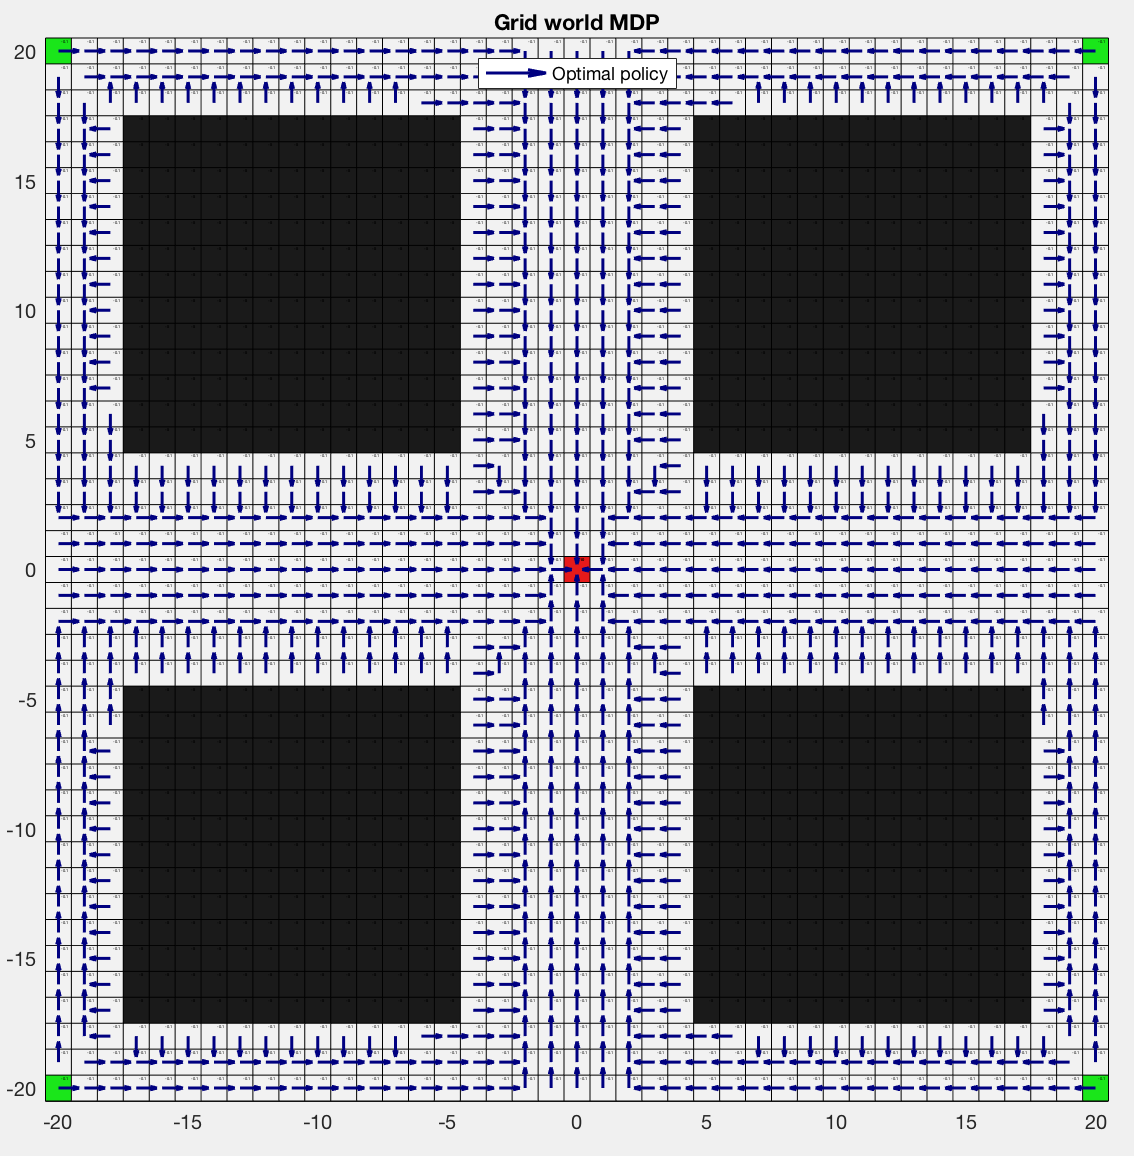
\includegraphics[width=\linewidth]{maze_optimal_policy}
					\caption{Optimal policy (value iteration)}
					\label{fig::maze_optimal_policy}
				\end{minipage}
			\end{figure}
				
			\paragraph{} If we go back at one of our motivating example (robot grasping an object), we could easily draw parallels between such an example and the grid environment we just presented. Indeed, we could imagine a teacher providing a demonstration that borders the obstacle. Because the learner suffers a (slightly) stochastic dynamic, this would indeed be a largely suboptimal solution, since large negative rewards will be likely to occur during the learning. However, the demonstration contains a fairly important information, that is the direction to follow to reach the center of the grid. 
						
			\paragraph{} Figure (\ref{fig::comp_maze}) displays the convergence (expressed as average reward on minibatch) for Q-learning, Sarsa($\lambda$), Sarsa(0) and Watkins Q($\lambda$). By average reward on minibatch, we mean that at every iteration, the reward is average around a given number of trajectories, following the same \emph{exploratory} policy. This allows to reduce the stochasticity of trajectories while learning and give a smoother estimation of how well the algorithm is learning. As a way of comparing them to the optimal and random policies, we also plot the average rewards perceived by the latest along many trajectories. \newline
For all the learning algorithms tested, we used optimistic action-value initialisation to promote exploration. This explains why many negative rewards are perceived in the beginning. 
				
			\begin{figure}
				\begin{center}
					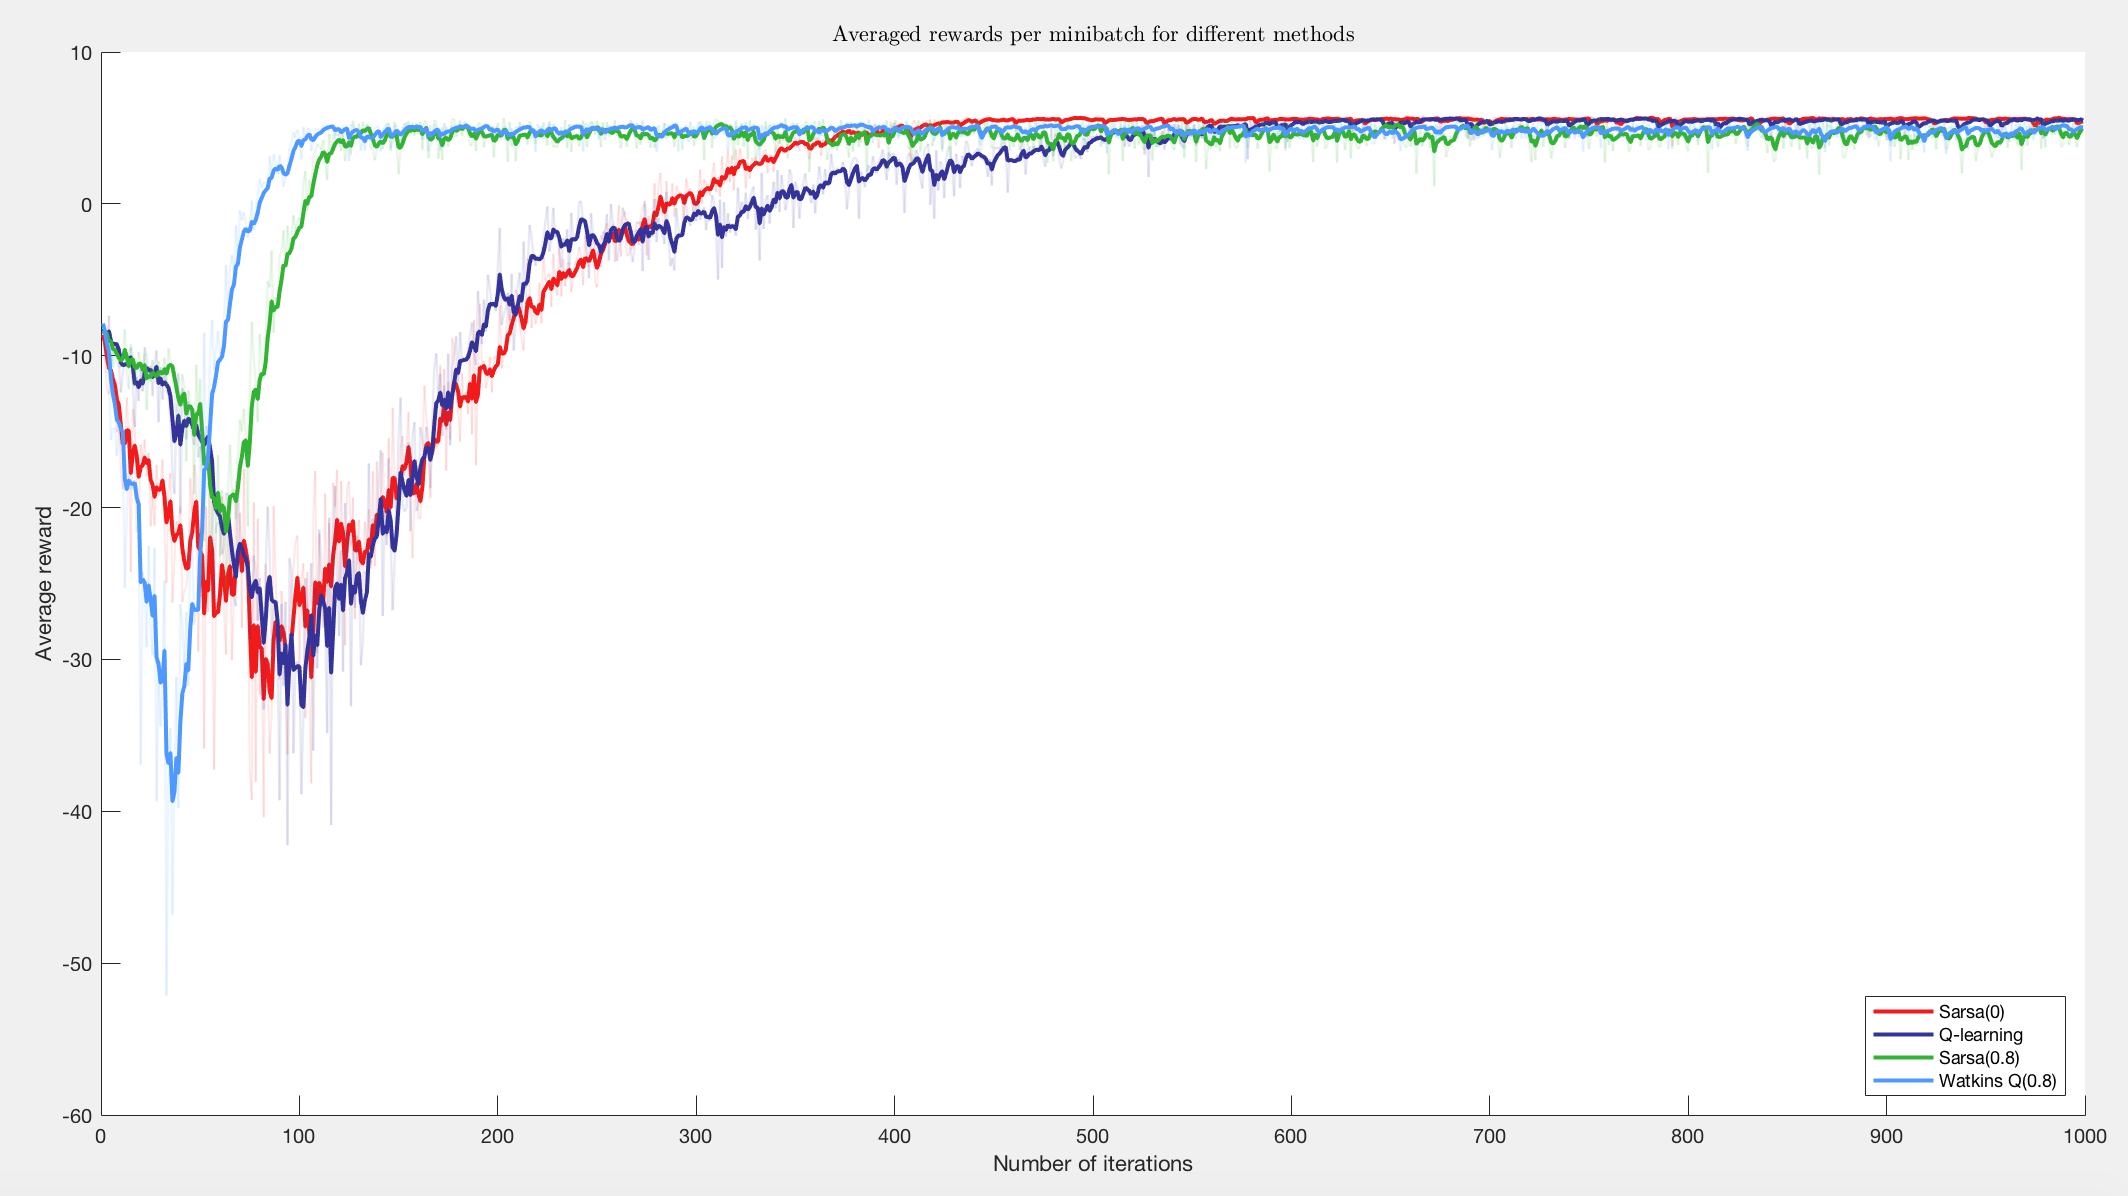
\includegraphics[width=\linewidth]{comp_maze}
					\caption{Average rewards on minibatch for learned policies, optimal policy and random policy.}
					\label{fig::comp_maze}
				\end{center}
			\end{figure}
		}
	\section{Generating mentors}
	{
	
		\begin{figure}[h!]
			\begin{center}
				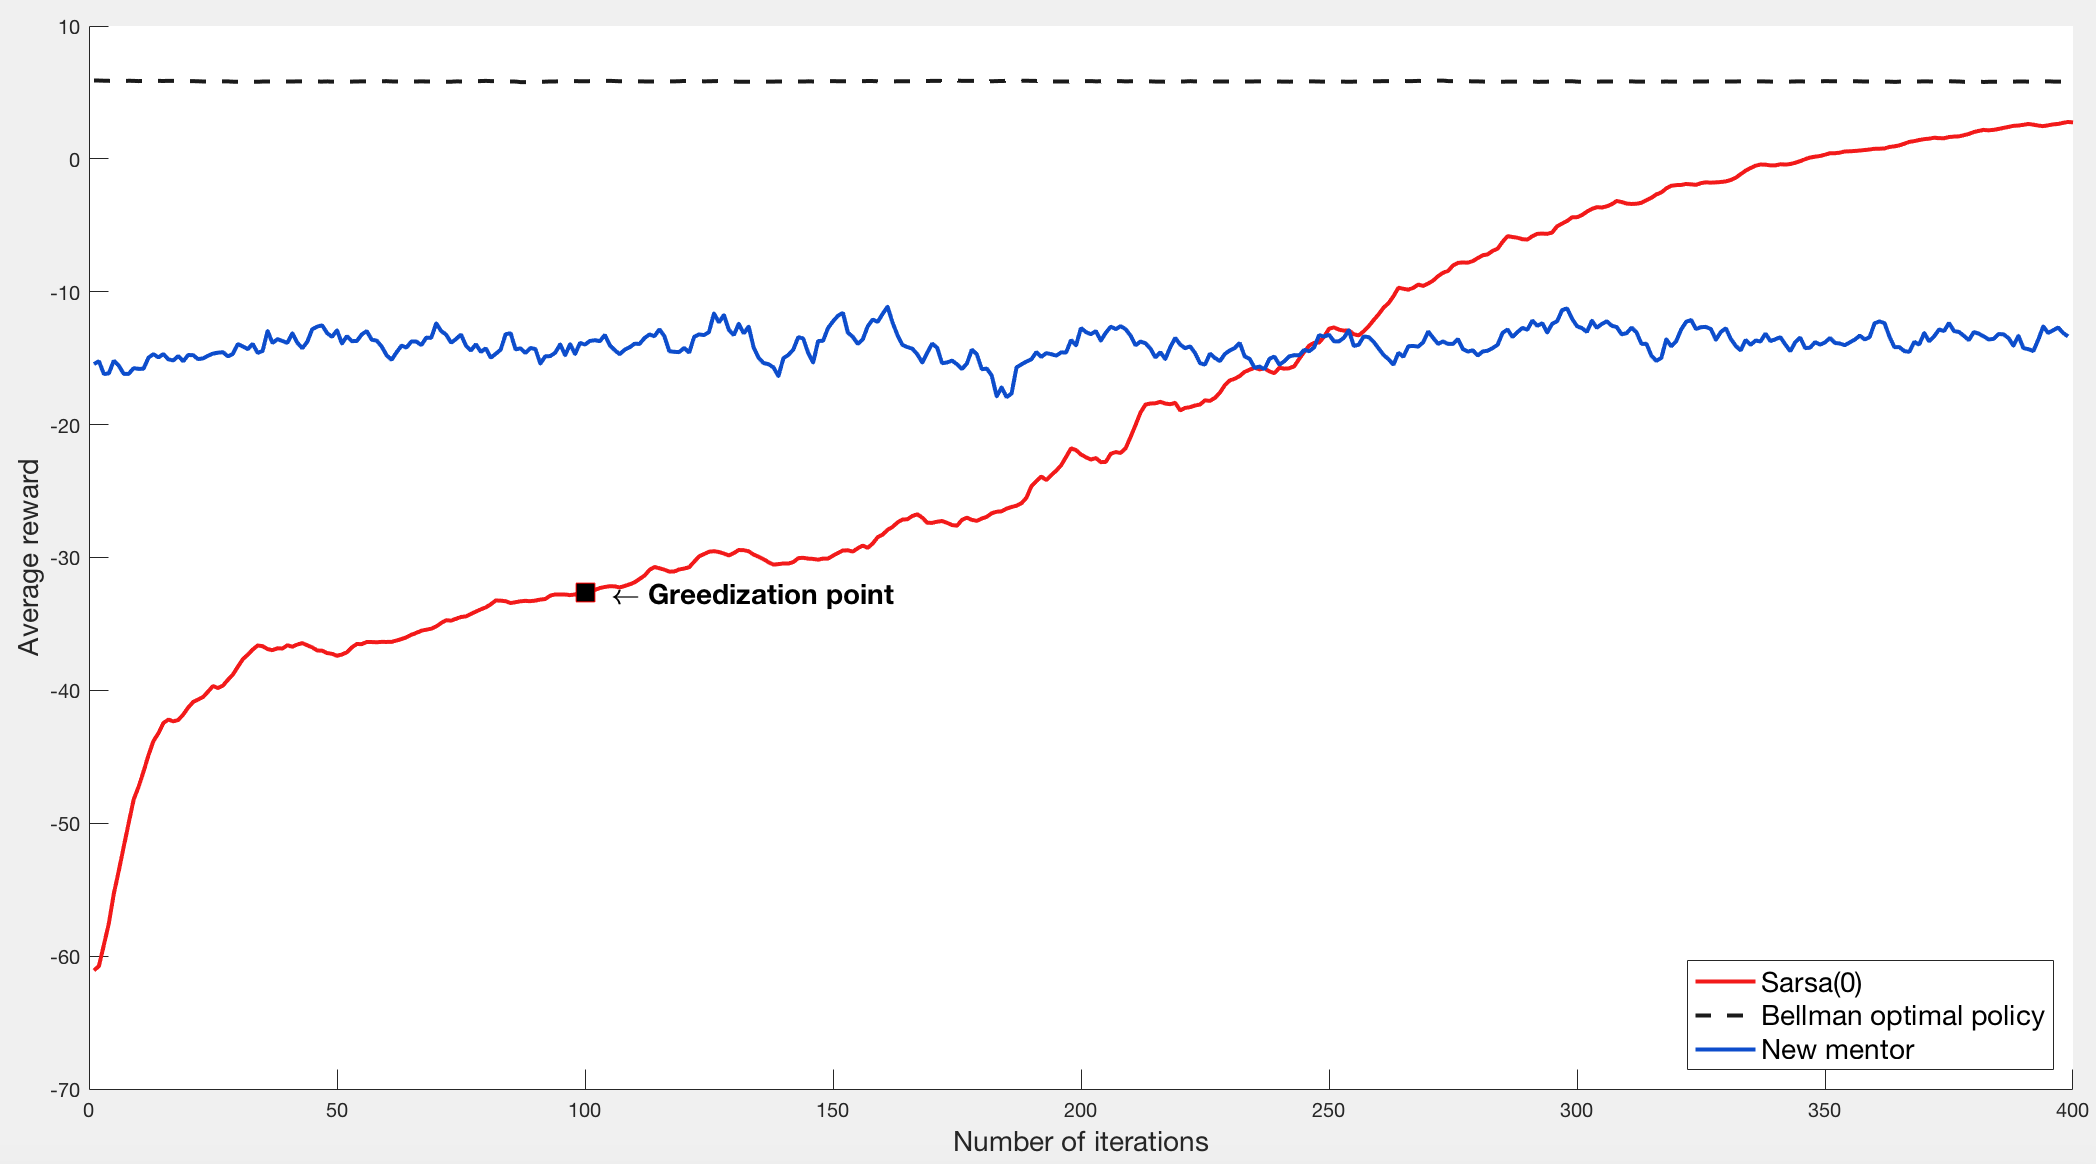
\includegraphics[width=0.7\linewidth]{mentor_gen}
				\caption{Generating a suboptimal mentor from a SARSA learner}
				\label{fig::mentor_gen}
			\end{center}
		\end{figure}
		
		\paragraph{} Besides giving us an idea on how generic reinforcement learning algorithms performs on our sandbox MDP, those different reinforcement learning methods enable us to \emph{generate mentors of varying sub-optimal levels}. 
		
		\paragraph{} If we consider a SARSA learner (for instance), we can at any time of its learning generate a deterministic version of the current exploratory policy. This is done by taking its greedy version with respect to its current Q-values estimates. Hence $\forall s\in\mathcal{S}$: 
		\begin{equation}
			\pi_m(s) = \argmax{a\in\mathcal{A}(s)}{Q(s,a)}
		\end{equation}
		
		Such a process is displayed in figure (\ref{fig::mentor_gen}). Because the mentor's policy is deterministic, it is slightly better than the learner it was generated from, but still is clearly suboptimal. This method hence enables us to generate mentor of different optimality levels. 
	}
	\section{Naive learners}
	{
		\label{section::naive_learners}
		\subsection{Constant compliance learner}
		{
			\paragraph{} In the context of the action-selection process described in (\ref{eq::compliant_exploration}), we decided to first implement a fairly naive method. It consists in following the teacher's recommandation with a \textbf{constant} compliance term $p$: the learner \emph{complies} with the teacher with probability $p$, and decide to choose its own action (that \textbf{could include} $\boldsymbol{a_m}$) with probability $1-p$. This is a slight digression from (\ref{eq::compliant_exploration}), that is made here to enable a learner to reach optimality. The softmax sampling used when discarding a recommandation is tuned by a decaying temperature coefficient, making it greedy in limit.
			
			\paragraph{} The figures (\ref{fig::comp_opt_verynaive}) and (\ref{fig::comp_subopt220_verynaive}) display the learning curves obtained when fed with, respectively, the optimal policy for the MDP and a slightly suboptimal one. 
			
			\begin{figure}[ht!]
				\begin{minipage}{0.5\linewidth}
					\begin{center}
						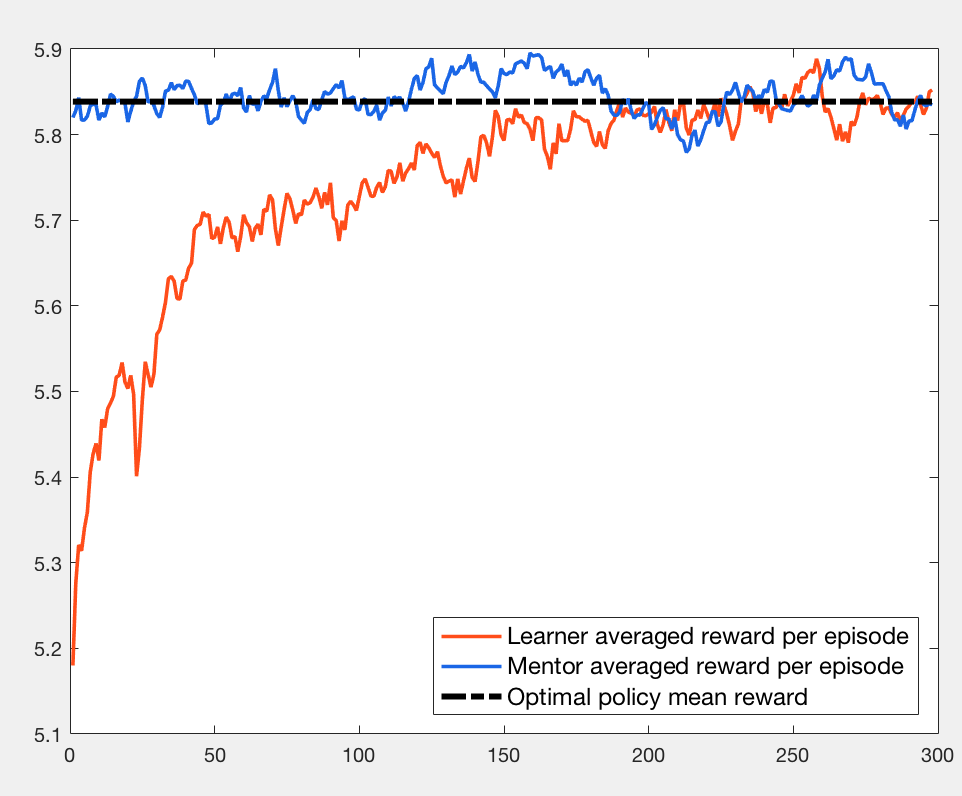
\includegraphics[width=0.9\linewidth]{very_naive_opt}
						\caption{Constant compliance learning, $p=0.9$, with the optimal mentor}
						\label{fig::comp_opt_verynaive}
					\end{center}
				\end{minipage}
				\begin{minipage}{0.5\linewidth}
					\begin{center}
						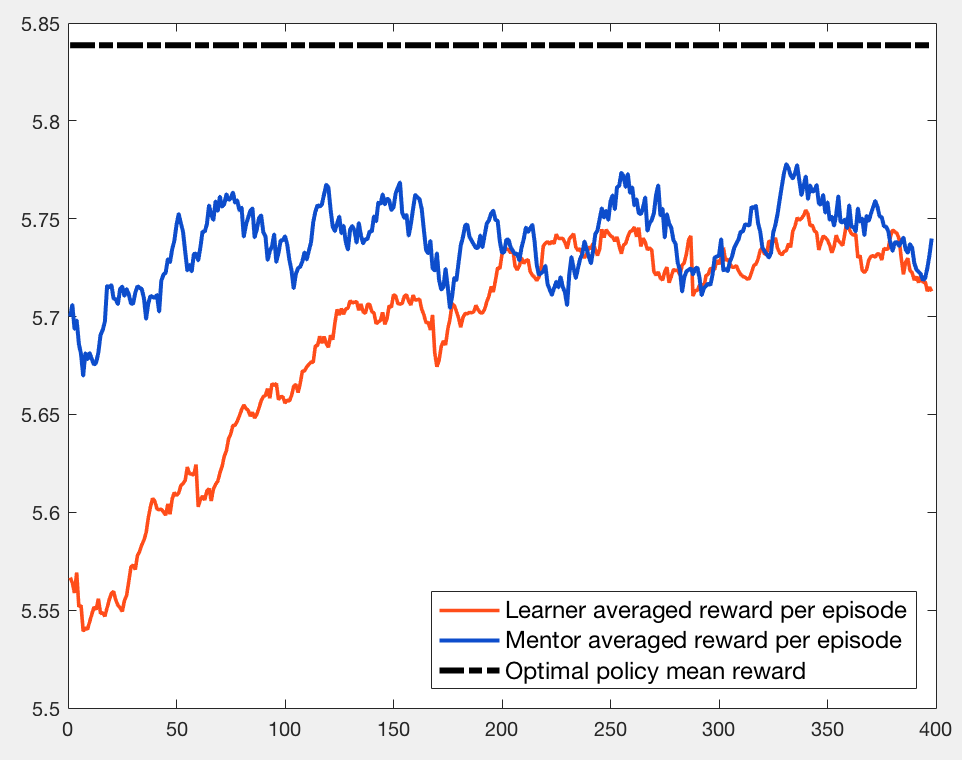
\includegraphics[width=0.9\linewidth]{very_naive_200}
						\caption{Constant compliance learning, $p=0.9$, with a slightly suboptimal mentor}
						\label{fig::comp_subopt220_verynaive}
					\end{center}
				\end{minipage}
			\end{figure}
	
			\paragraph{} Figure (\ref{fig::comp_opt_verynaive}) shows that from its exploration, the learner is able to quickly learn his way thanks to the optimal mentor. As expected, it eventually follows the mentor's action, wether it complies or not, since the recommended action holds the best action-values. On the other hand, as shown in figure (\ref{fig::comp_subopt220_verynaive}), the high confidence the learner initially have in its mentor prevents it from reaching optimal performance, and the policy its renders actually mimic its mentor suboptimal one. Still, one could expect the learned policy to be slightly better than its suboptimal teacher's one, even if not optimal. However, achieving this comes with a lot of effort in the tuning of $p$ and of the softmax distribution temperature decrease coefficient. 
	
			\begin{figure}[ht!]
				\begin{center}
					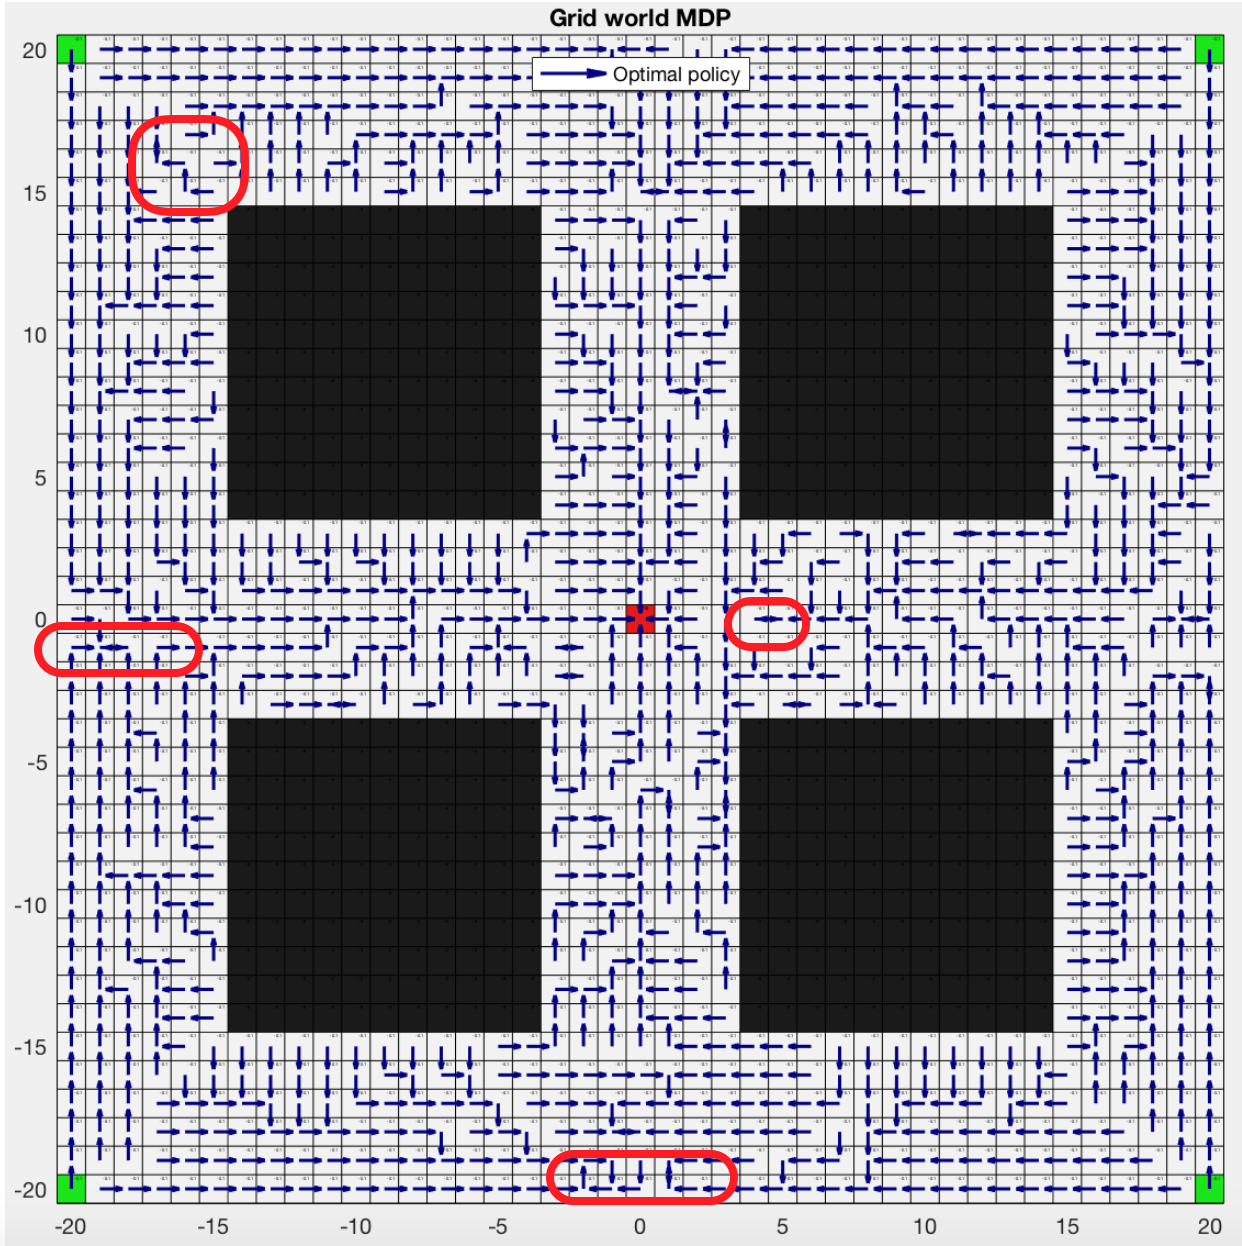
\includegraphics[width=0.7\linewidth]{subopt_policy_block}
					\caption{An exemple of suboptimal mentor policy that doesn't always lead to the positive reward}
					\label{subopt_policy_block}
				\end{center}
			\end{figure}
			
			\paragraph{} This remark actually pinpoints a major downside of this method, that is the need of fine tuning of the parameter $p$. But obviously, there is even a bigger downside, which becomes a major game killer when dealing with largely suboptimal mentors. Indeed, some mentors can be suboptimal enough to only show a good direction of exploitation, but not be able to reach the target. Figure (\ref{subopt_policy_block}) displays such a policy, where the mentor's policy creates loops and does not always leads to the positive reward.  \newline
			Applying the latest method with such a teacher is fatal for the learning, as the learner discovers that following the mentor's action yields largely negative rewards, but is not able to bypass them as it keeps a constant confidence in its teacher. This leads the learner to build up low Q-values in the directions recommended by the mentor, and to try to follow an opposite path. This is highly counter-productive since the mentor still gives the right exploration direction. 
		
		\subsection{Vanishing compliance learner}
		{
			\paragraph{} One of the downside of the constant compliance approach is that the exploratory behavior is always biased by the mentor's recommandation. This breaks the need of this policy to be \emph{greedy in limit} (which is a specification for SARSA algorithm to converge). In the case of a sub-obptimal mentor, this means that the optimal behavior could never be reached. 
			
			\paragraph{} We now decide to comply with the need to be greedy in limit. Therefore, we decide to set $p$ to be \emph{constantly decreasing along the learning}: 
			\begin{equation}
				p_{t+1} = \beta p_{t}
			\end{equation}
			with $\beta < 1$. 
			
			\paragraph{} The action-selection is therefore biased by the mentor's recommandation in the beginning of the learning only, and slowly decides to take its own choices, based on its current Q-values estimates. This approach sounds more promising as the learner is more likely to quickly discover the location of high rewards (following the teacher policy with $p$ close to 1), and will then makes it own exploration along those trajectory, to end up in a setting where the teacher's actions are now longer considered. 
		
			\begin{figure}[ht!]
				\begin{minipage}{0.5\linewidth}
					\begin{center}
						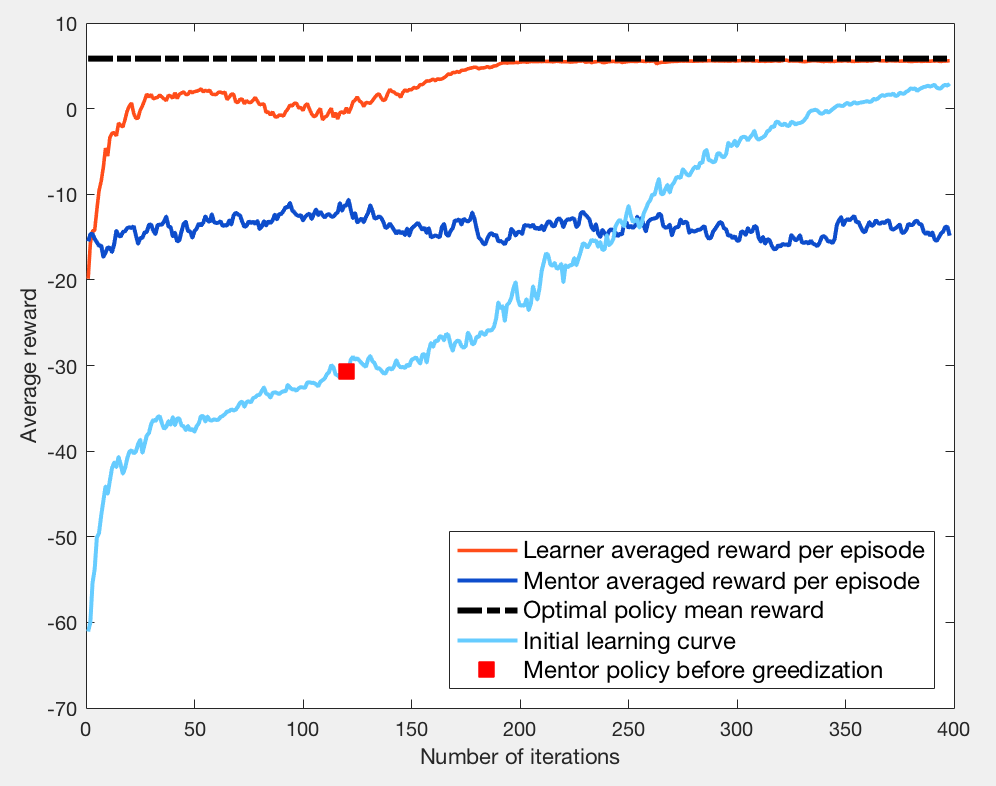
\includegraphics[width=0.95\linewidth]{comp_naive_compliance_120}
						\caption{Vanishing compliance, $\beta = 0.99$}
						\label{fig::comp_naive_compliance_120}
					\end{center}
				\end{minipage}
				\begin{minipage}{0.5\linewidth}
					\begin{center}
						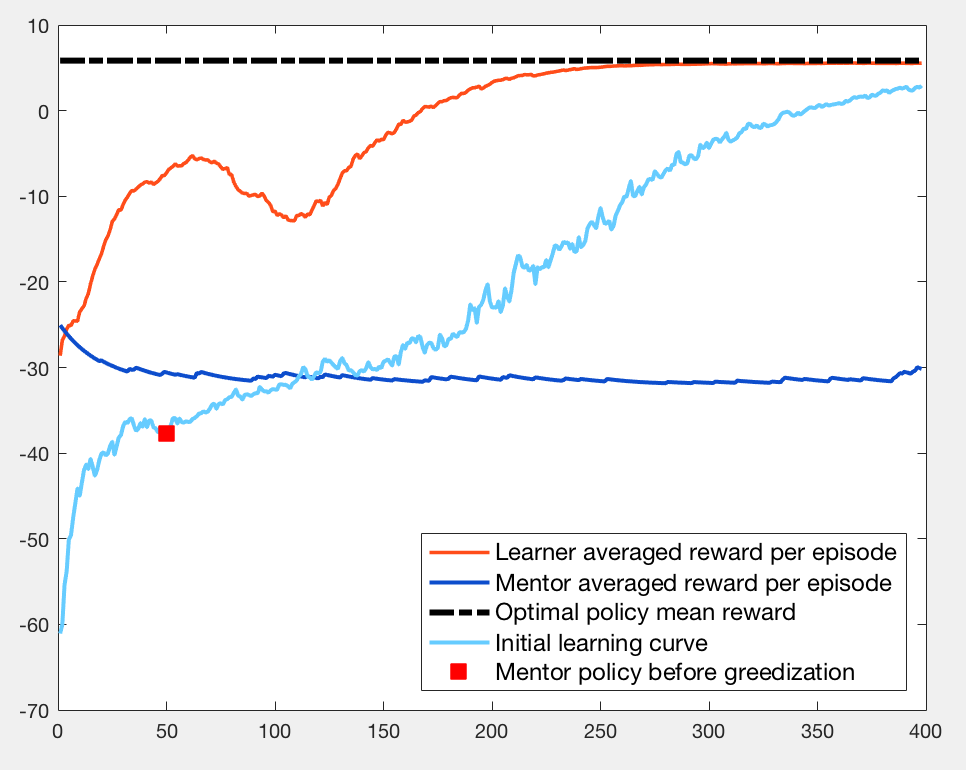
\includegraphics[width=0.95\linewidth]{comp_naive_compliance_50}
						\caption{Vanishing compliance, $\beta = 0.97$}
						\label{fig::comp_naive_compliance_50}
					\end{center}
				\end{minipage}
			\end{figure}
			
			\paragraph{} Figures (\ref{fig::comp_naive_compliance_120}) and (\ref{fig::comp_naive_compliance_50}) display the result on two sub-optimal policies, that were derived from the Q-values learned at a given moment (denoted through a red square) in a learning process. They show that with this approach, while the learner is compliant with the teacher, it steadily increases its accumulated reward thanks to its exploratory actions. However, it then comes to a plateau (or even an undershoot) when the guidance by the teacher becomes too weak as $p$ reaches a critical level. The learner then mostly relies on its exploratory actions (which volatility are guided by its temperature coefficient) to explore new regions of the state space. Once it has somehow learnt the action value function related to this part of its state space, and as its temperature goes down, the learner's accumulated reward goes up until it reaches the level of the optimal policy. 

		}		
		
		\paragraph{} If this approach seems to work relatively well, there are still some critical downsides to it. First of all, a lot of tuning is required in order to find the hyper-parameters ($p_0$, $\beta$, temperature evolution, ..) that lead to a fast learning. Also, there is an undershoot in the learning that seems to slow it down, due to the exploring phase that happens when $p$ becomes too low. Such exploration could be avoided or reduced if the learner is able to figure out quickly that indeed, the mentor was right in its recommandation.
		
		\paragraph{} This last remark is a clear motivation to search for better behaving confidence dynamics. Indeed, why automatically reject a recommandation (which is what the vanishing compliance does in the end of its learning) when we have all the information needed to state that this recommandation is a good one ?
	}
	
	\section{Adaptative compliance learners}
	{	
		\label{section::adaptative_learners}
		\paragraph{} It makes sense to somehow \emph{learn} the optimal value of the confidence parameter $p$, so that we don't have to manually tune its evolution, and so that it can store how right the teacher recommandations are. Ideally, we would like $p$ to be near $0$ when the teacher provide a suboptimal action and $1$ when the recommended action is sampled from the optimal policy. The underlying problem is therefore to infer the optimality of the teacher in different regions of the state space. 
		
		\paragraph{}We hereinafter describe two methods which attempt to do so. Their respective experimental results as well as further discussion will be found in chapter (\ref{chap::res}).  
		
		\subsection{Implicit $\beta$-compliance}
		{
			\paragraph{}  Let us define the \emph{confidence} term $p$ locally for every state of the state space. For each $s\in\mathcal{S}$, $p(s)$ is given a Beta prior: $p(s)\sim \beta(\alpha(s),\beta(s))$ and represents the initial trust we have in a mentor's recommandation at state $s$. The initial values $\alpha_0$ and $\beta_0$ define the initial prior belief we have over $p$ (for instance, $\alpha=0.5$ and $\beta = 0.055$ define a prior belief that the teacher is most probably right). 
			
			\paragraph{} As in before, we perform a $\color{red}p$\textcolor{red}{\emph{-greedy policy}} with respect to the teacher recommandation: 
			\begin{equation}
				\forall s\in\mathcal{S}, \quad \pi_p(s) = 
					\left\{ 
					\begin{aligned}
						&a_m \text{ with probability } p(s) \\
						& a\in\mathcal{A}(s)\backslash{a_m} \text{ with probability } (1-p(s))
					\end{aligned}
					\right. 
			\end{equation}
			
		\begin{figure}[h!]
				\begin{center}
					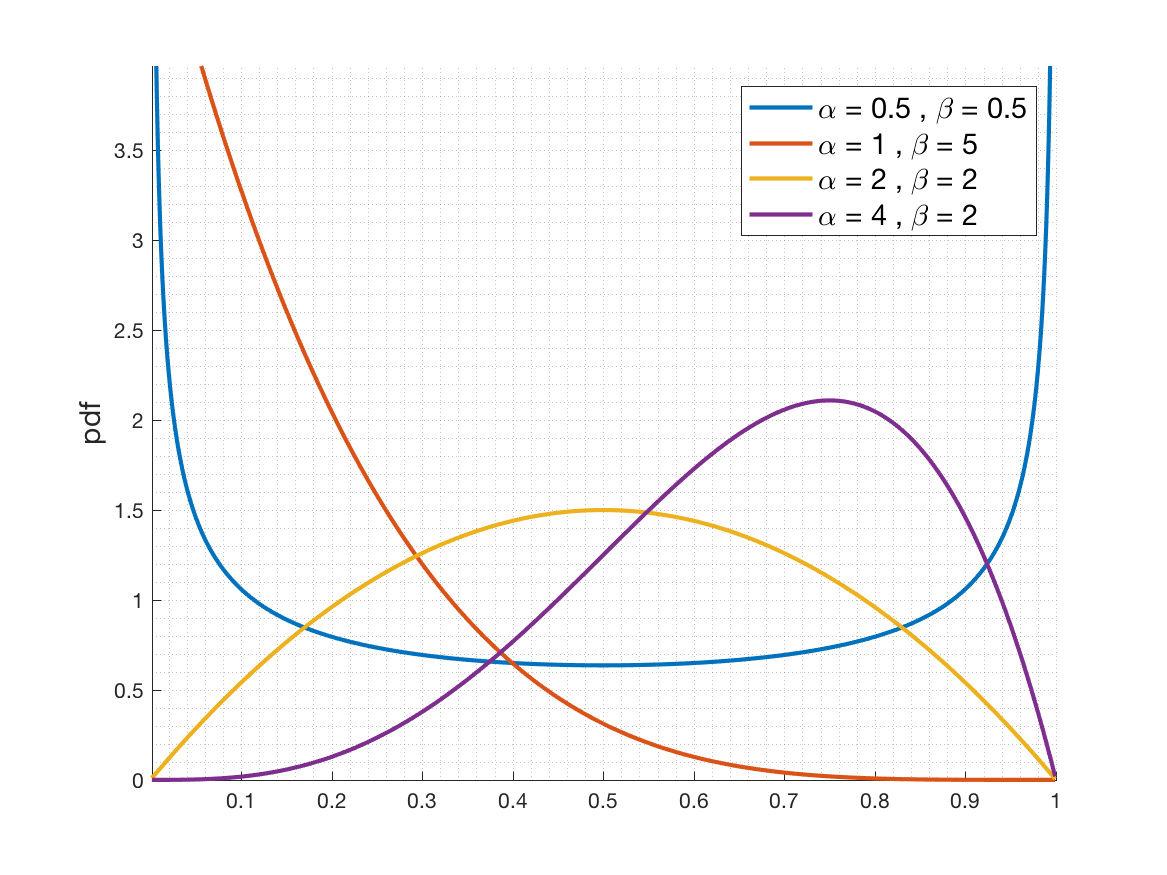
\includegraphics[width=0.55\linewidth]{Beta_distribution_pdf.png}
					\caption{The Beta distribution for several values of $(\alpha,\beta)$}
				\end{center}
			\end{figure}
			
		\paragraph{}The following describe how we wish to learn the value of $p(s)$, $\forall s\in\mathcal{S}$. Based on the $5$-tuple $(s,a,r,s',a')$ obtained thanks to the action selection process we just described, we compute at every step the following temporal difference value: 
			\begin{equation}
				\delta_t = r + \gamma Q(s',a') - Q(s,a_m)
			\end{equation}
			which compares, \emph{in average}, the advantage (our drawback) of following the state-action pair $(s,a)$ rather than the one indicated by the teacher, according to the current Q-values estimates. 
		
			\paragraph{} We then apply the following update rule to $p(s)$: 
			\begin{equation}
				\label{eq::update_rule}
				\begin{aligned}
					\alpha_t(s) &\leftarrow \alpha_t(s) +  \mathds{1}_{a=a_m}\delta_t \eps_t\\
					\beta_t(s) &\leftarrow \beta_t(s) +   \mathds{1}_{a\neq a_m}\delta_t \eps_t
				\end{aligned}
			\end{equation}
			The intuition behind this update rule is simple: if we see that the expected return for the mentor action increases (resp. decreases), then we increase (resp. decrease) $\alpha$ which results in a shift of $p$ toward a larger (resp. smaller) confidence. A similar reasoning holds for the $\beta$ term.  $\eps_t$ is the update rule's learning rate, which value and dynamic will be discussed later. 
		
		}
	
		\subsection{Explicit compliance}
		{
			\paragraph{} We consider here a somewhat similar approach, where our listen versus discard exploration policy is computed according to the current estimated values of the actions \emph{'listen'} and \emph{'discard'}. Let us introduce the action spaces: 
			\begin{equation}
				\forall s\in\mathcal{S}, \, \mathcal{A}_c(s) = \left\{ 'listen', \, 'discard'\right\}
			\end{equation}
			to which we assign the action values $Q_c(\cdot,l)$ and $Q_c(\cdot,d)$ (where $'l'$ denotes the action of listening and $'d'$ the action of discarding the teacher recommendation). 
			
			\paragraph{} The exploration is done by computing a soft policy derived from $\{Q_c(s,l), Q_c(s,d)\}$ for all $s\in\mathcal{S}$. We do this using a Gibbs softmax distribution, which yields: 
			\begin{equation}
				\forall s \in\mathcal{S}, \quad \pi_c(s) = 
					\left\{
						\begin{aligned}
							&'l' \text{ with probability } p=\sigma\left(\frac{Q_c(s,l) - Q_c(s,d)}{\tau} \right) \\
							& 'd'  \text{ with probability } 1-p
						\end{aligned}
					\right.
			\end{equation}
			where $\sigma(\cdot)$ is the logistic sigmoid and $\tau$ is a temperate coefficient decreasing to $0$ (greedy policy in limit). 
			
			\paragraph{} After each SARSA update, we also make the following update: 
			\begin{equation}
				\label{eq::av_update_rule}
				\left\{
				\begin{aligned}
					&Q_c(s,l) \leftarrow  \beta Q_c(s,l) + (1-\beta)Q(s,a_m) \\
					&Q_c(s,d) = \beta Q_c(s,d) + (1-\beta)\max_{a\neq a_m} Q(s,a) 
				\end{aligned}
				\right.
			\end{equation}
			with $\beta >0$ the update rule's learning rate. 
			\paragraph{} We can introduce some prior confidence in the teacher by setting, $\forall s\in\mathcal{S}$: 
			\begin{equation}
				Q^0_c(s,l) - Q^0_c(s,d) =\tau \log\{\frac{p}{1-p}\}
			\end{equation}
			where $p$ is the retained probability of initially choosing to listen to the teacher. 
			}
		}	
	}
	
	\chapter{Results}
	{
		\label{chap::res}
				\paragraph{} The following sections procide some practical considerations for the implicit $\beta$-compliance and explicit compliance methods, and discuss the experimental results we obtained. 
		\section{Implicit $\beta$-compliance}
		{
			\subsection{Practical considerations}
			{
				\paragraph{} One of the main specification of the SARSA learning paradigm is that the exploration policy must be \emph{greedy in limit} so that a fixed point can emerge (hopefully the set of Q-values related to the optimal policy). In an actor-critic approach, the usual way to bring the \emph{critic} term in a stationary regime is to modify its learning rate to take the probability of taking an action into account (see \cite{Sutton98a}). \newline
				This is the approach we chose in order to pick the learning rate $\eps_t$ of the update rule (\ref{eq::update_rule}), which now becomes: 
			\begin{equation}
				\begin{aligned}
					\alpha_t(s) &\leftarrow \alpha_t(s) +  \mathds{1}_{a=a_m}\gamma \delta_t(1- p(s))\\
					\beta_t(s) &\leftarrow \beta_t(s) +   \mathds{1}_{a\neq a_m}\gamma \delta_t p(s)
				\end{aligned}
			\end{equation}
			with $\gamma >0$. This update rule can still be simplified, by approximating $p$ by its mean value, which gives the update rule that we applied in practice: 
			\boxedeq{red}
			{
				\begin{aligned}
					\alpha_t(s) &\leftarrow \alpha_t(s) +  \mathds{1}_{a=a_m} \frac{\gamma \beta_t(s)}{\alpha_t(s) + \beta_t(s) }\delta_t \\
					\beta_t(s) &\leftarrow \beta_t(s) +   \mathds{1}_{a\neq a_m} \frac{\gamma \alpha_t(s) }{\alpha_t(s) + \beta_t(s) } \delta_t
				\end{aligned}
			}
			This ensures us that we will direct the update toward a fixed point, and end up with a greedy exploratory policy (in limit). 
			
			\paragraph{} In this method, $p$ is given a Beta prior distribution. To perform the action selection, we would therefore need to sample $p(s)$ from its current distribution, and then sample a Bernoulli random variable of parameter $p(s)$. Assuming that the Beta distribution is sharply peaked around its mean (which we will guarantee by choosing an appropriate prior and learning rate $\gamma$). Then $p(s)$ can be approximated by its mean value $\E{p(s)} = \displaystyle\frac{\alpha(s)}{\alpha(s) + \beta(s)}$. We therefore only need to sample a Bernoulli random variable of parameter $\E{p(s)}$ at every state to complete the action selection process. 
			
			\paragraph{} The tuning that needs to be done is therefore left to $\gamma$, the prior and the temperature. In this framework, tuning is made much simpler and one only has to check that the updates are of the same order of magnitude with the prior (in order for the posterior distribution to adapt to observations, but also to retain the memory of the prior). 
			}
			\subsection{Results}
			{
				\paragraph{} Figures (\ref{fig::ac_il_subopt_120}) and (\ref{fig::ac_il_subopt_50}) show the learning curves for an agent using the $\beta$-compliance, with two different suboptimal teachers (generated from a SARSA learner, indicated by the red square). 
				
				\begin{figure}[ht!]
					\begin{minipage}{0.5\linewidth}
						\begin{center}
							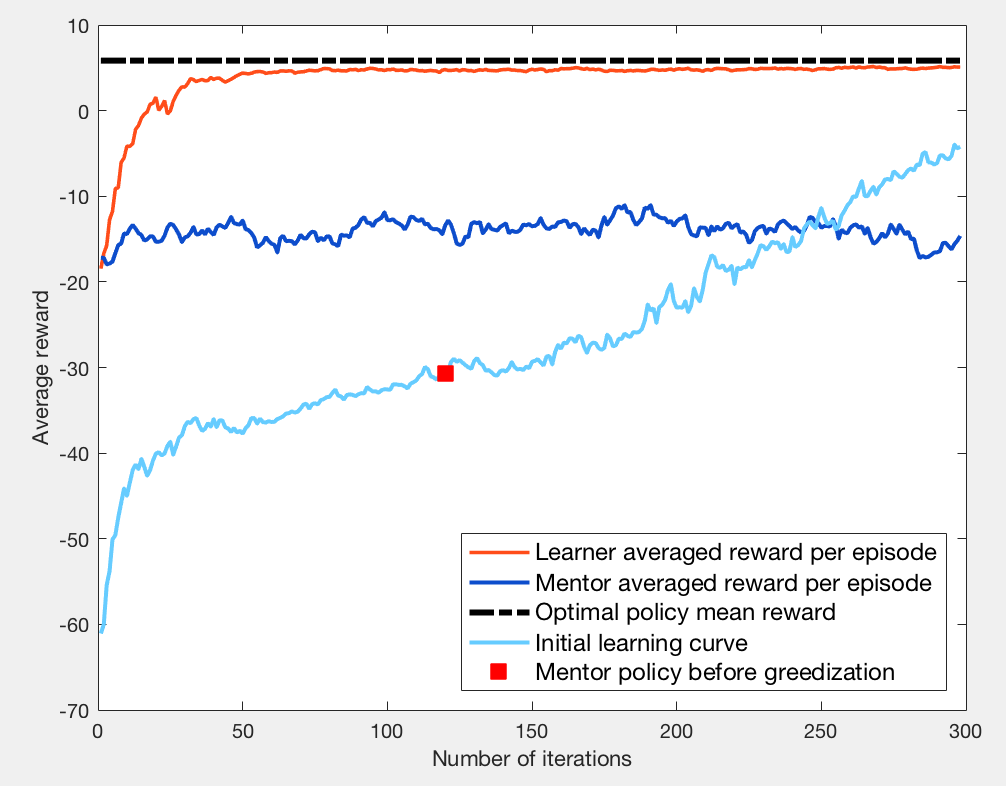
\includegraphics[width=0.95\linewidth]{ac_il_subopt_120}
							\caption{$\beta$-implicit compliance learning curve}
							\label{fig::ac_il_subopt_120}
						\end{center}
					\end{minipage}
					\begin{minipage}{0.5\linewidth}
						\begin{center}
							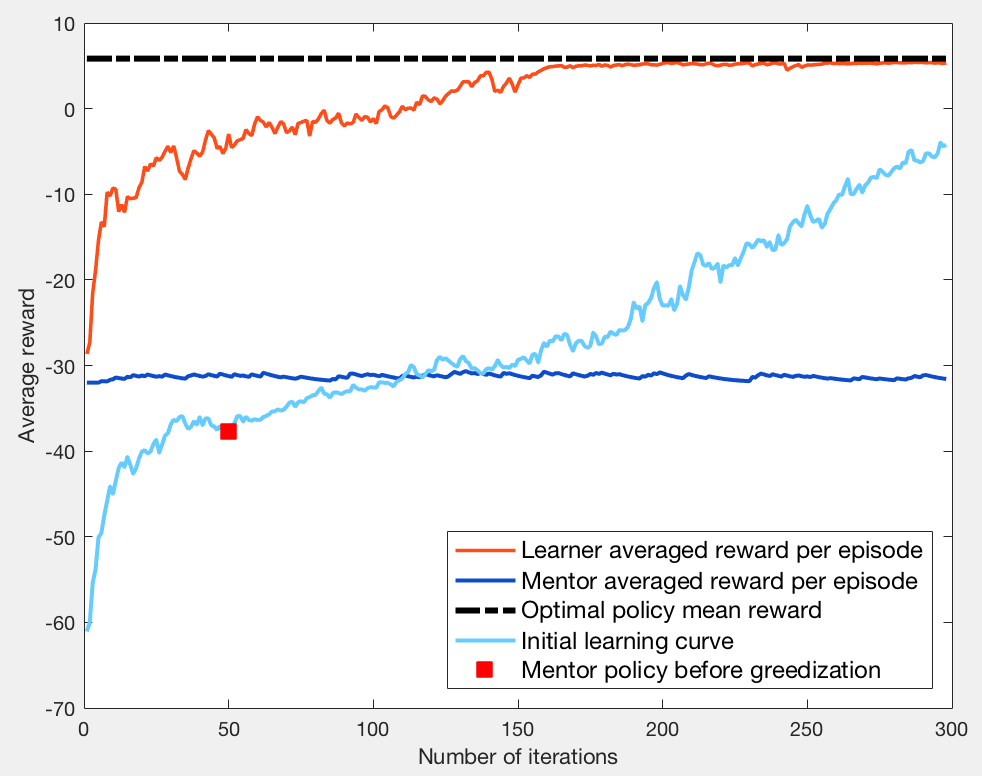
\includegraphics[width=0.95\linewidth]{ac_il_subopt_50}
							\caption{$\beta$-implicit compliance learning curve}
							\label{fig::ac_il_subopt_50}
						\end{center}
					\end{minipage}
				\end{figure}
				
			\paragraph{} The first remark we can make is that by learning the confidence, we were able to avoid the undershoot that we observed for the vanishing compliance method (see figures (\ref{fig::comp_naive_compliance_120}) and (\ref{fig::comp_naive_compliance_50})). This results in a faster learning and better behaving learning curves. The different methods will be further compared in (\ref{sec_method_comp}). 
			}
			\subsection{Discussion}
			{
				\paragraph{} It would be interesting to see what is the \emph{posterior distribution} of the $\{p(s)\}_{s\in\mathcal{S}}$. We expect our final policy to be greedy, and hence the posterior distribution of the compliance term to be sharply peaked around $0$ or $1$, with proportion given by how optimal the mentor is. Figures (\ref{fig::post_mean_120}) and (\ref{fig::post_mean_50}) display the histogram of the repartition of the $\E{p(s)}$ for $s\in\mathcal{S}$ (again, we approximate the Beta distribution by its mean to have an understandable visualization), for two suboptimal mentors. As expected, most of the means are either close to $0$ and $1$, and they are more means close to 0 (poor confidence) when using the second mentor - that is far worse than the first. 
				
				\begin{figure}[ht!]
					\begin{minipage}{0.5\linewidth}
						\begin{center}
							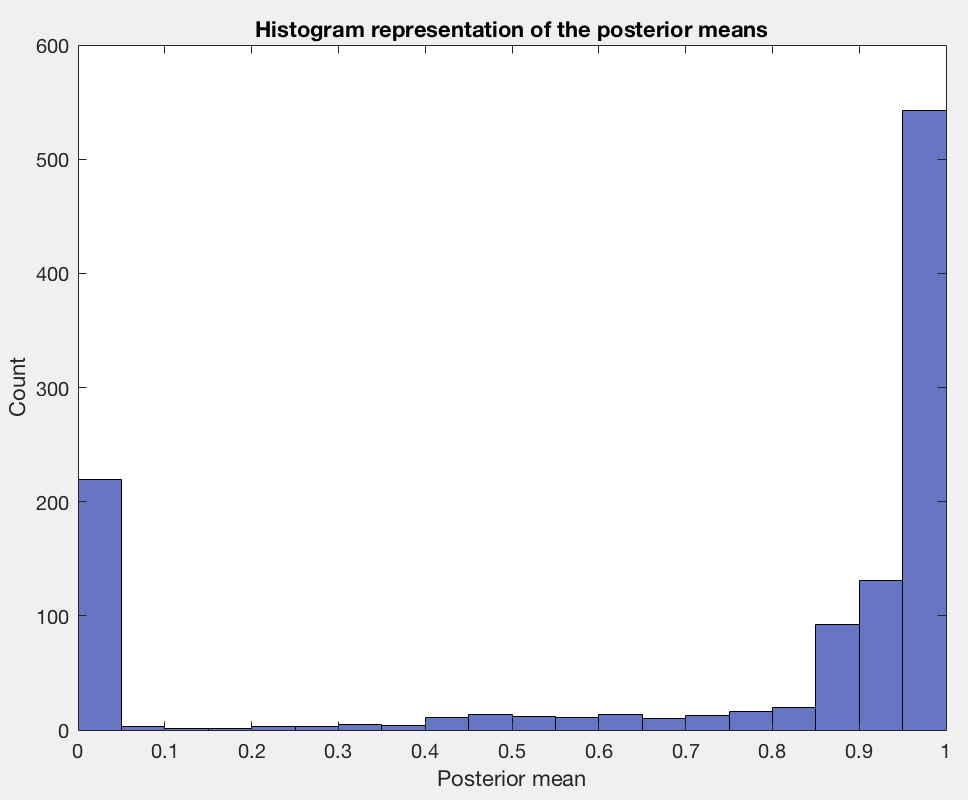
\includegraphics[width=0.95\linewidth]{post_mean_50}
							\caption{Histogram representation of the posterior means for a suboptimal teacher (first mentor)}
							\label{fig::post_mean_120}
						\end{center}
					\end{minipage}
					\begin{minipage}{0.5\linewidth}
						\begin{center}
							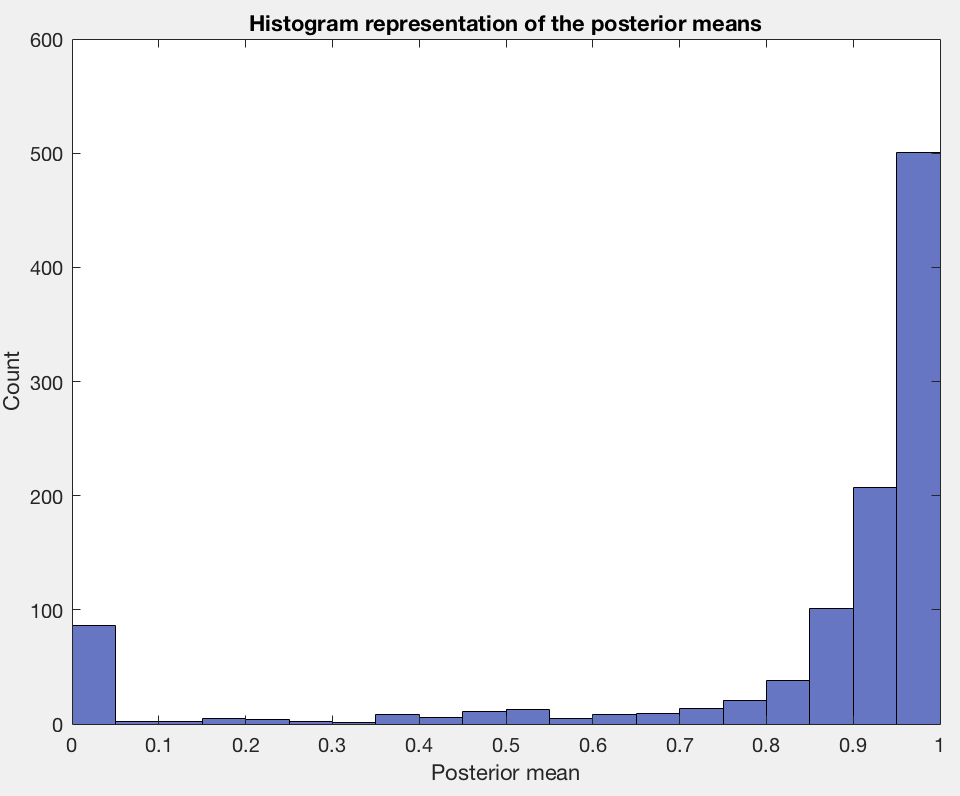
\includegraphics[width=0.95\linewidth]{post_mean_120}
							\caption{Histogram representation of the posterior means for a a suboptimal teacher (second mentor)}
							\label{fig::post_mean_50}
						\end{center}
					\end{minipage}
				\end{figure}
				
				\paragraph{} Also, to better understand how this algorithm works, it would be interesting to visualize the areas where the learner rejects or listen to its mentor. We expect the learner to discard the mentor's recommandations where those are wrong, and to trust its mentor where it is right (compared to the actions of an optimal policy). Figures (\ref{fig::heatmap_confidence_120}) and (\ref{fig::heatmap_confidence_50}) display, for two different mentors (the same two ones as we just used), the mentor's policy and the heat-map of the confidence the learner as acquired with respect to its teacher's recommandation at the end of the learning. Red arrows indicate a confidence close to 0, when green arrows are for confidence close to 1. 
				
				 \begin{figure}[ht!]
					\begin{minipage}{0.5\linewidth}
						\begin{center}
							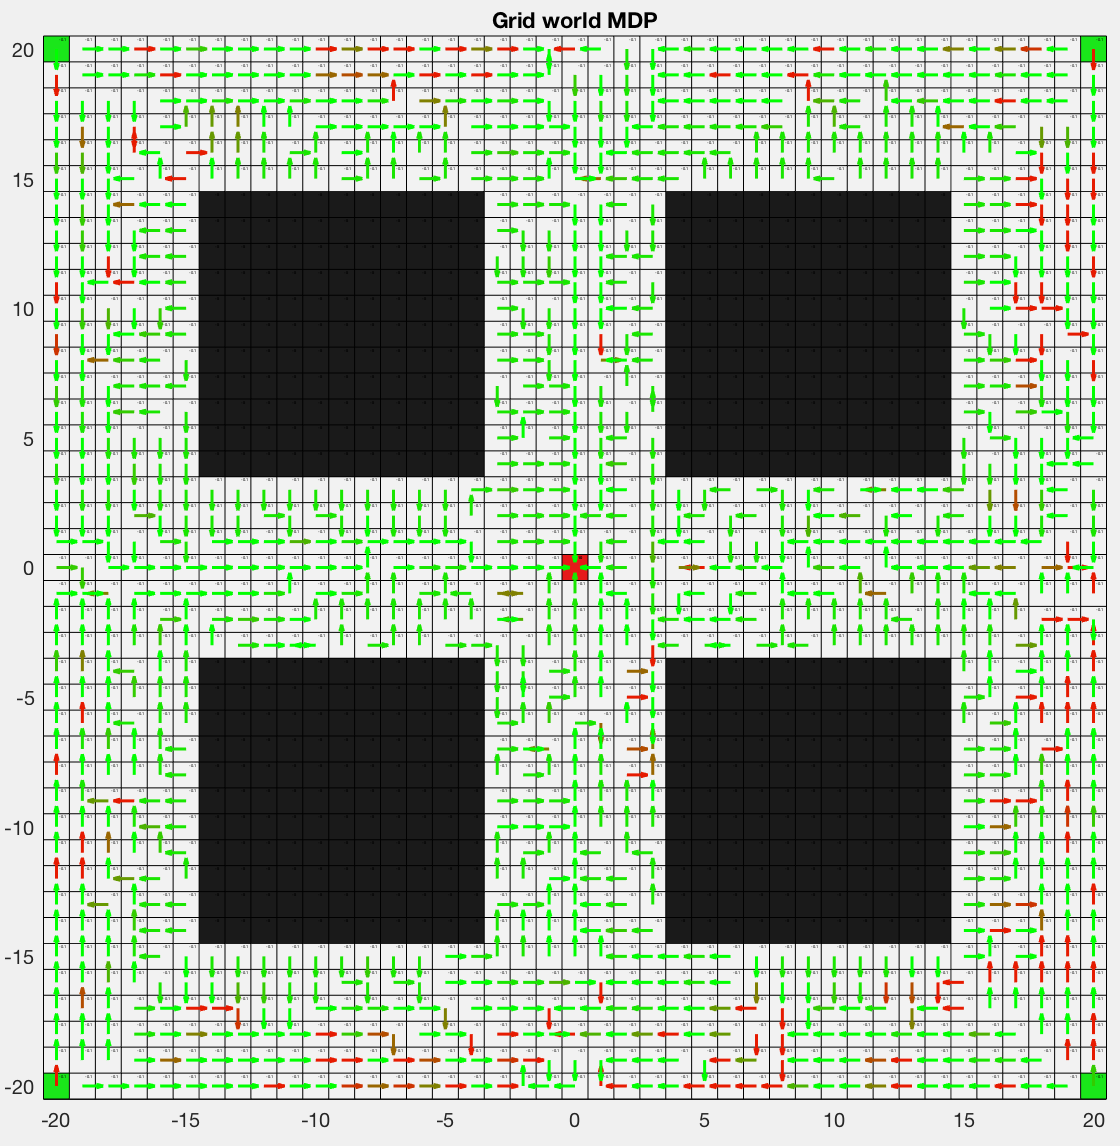
\includegraphics[width=0.95\linewidth]{heatmap_confidence_120}
							\caption{Learnt confidence: green arrows show near 1 posterior mean, red arrows near 0}
							\label{fig::heatmap_confidence_120}
						\end{center}
					\end{minipage}
					\begin{minipage}{0.5\linewidth}
						\begin{center}
							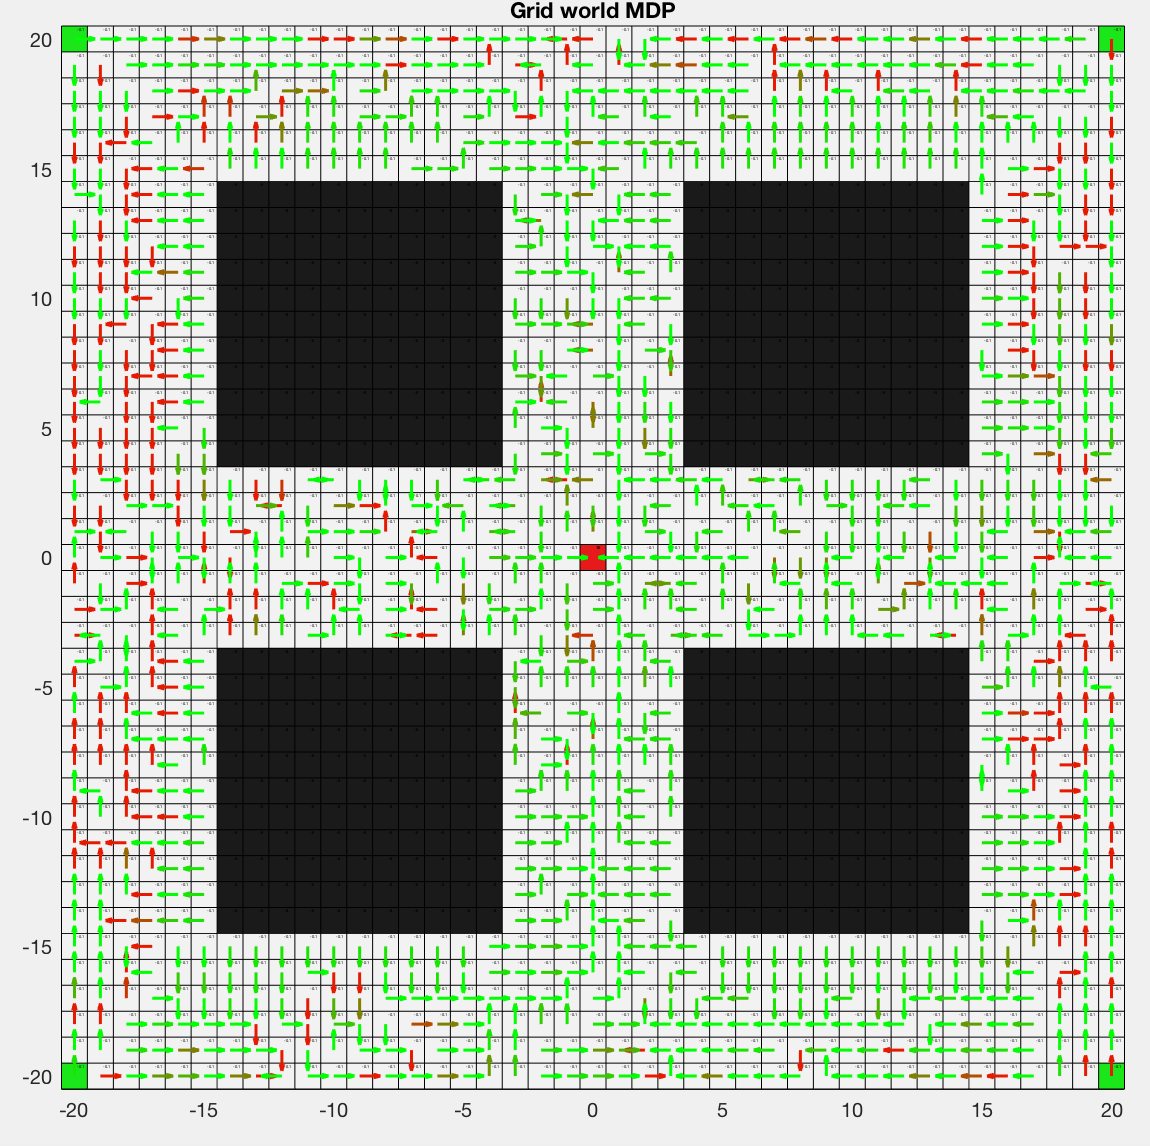
\includegraphics[width=0.95\linewidth]{heatmap_confidence_50}
							\caption{Learnt confidence: green arrows show near 1 posterior mean, red arrows near 0}
							\label{fig::heatmap_confidence_50}
						\end{center}
					\end{minipage}
				\end{figure}
				
				\paragraph{} The first observation one can make is that most of the suboptimal mentor actions are indeed well classified by the learner (red arrows). Also, most of the actions leading to such actions are also classified as poor recommandations, because they have a tendency of leading to deadlocks, or suboptimal actions.  
			}
		}
		\section{Explicit compliance}
		{
		
			\subsection{Practical considerations}
			{
				\paragraph{} The implementation of this method is rather straight forward and contains no major difficulties. However, some hyper-parameters have to be tuned, like the two temperatures for action-selection (since we are updating two different MDP action-value tables) as well as their respected  dynamics (multiplicative factor) and the learning rate of the update rule (\ref{eq::av_update_rule}). 
				
				\paragraph{} In practice, this tuning is rather easy to perform, as long as one make sure that the initial values for $Q_c(s,l)$ and $Q_c(s,d)$ ($s\in\mathcal{S}$) don't absorb the observations but also retain some prior knowledge along the learning (the learning rate $\beta$ has to be related to those initial values in some way). 
			}
			\subsection{Results}
			{				 
				 \begin{figure}[ht!]
					\begin{minipage}{0.5\linewidth}
						\begin{center}
							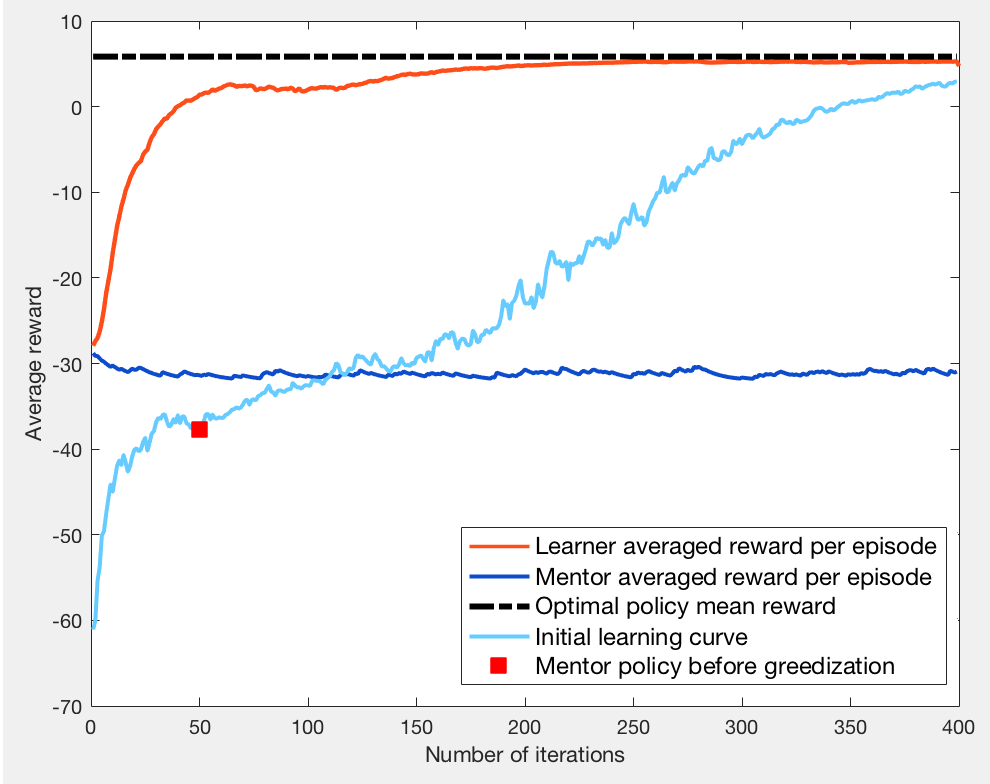
\includegraphics[width=0.95\linewidth]{av_il_subopt_120}
							\caption{Explicit compliance learning curve}
							\label{fig::av_il_subopt_120}
						\end{center}
					\end{minipage}
					\begin{minipage}{0.5\linewidth}
						\begin{center}
							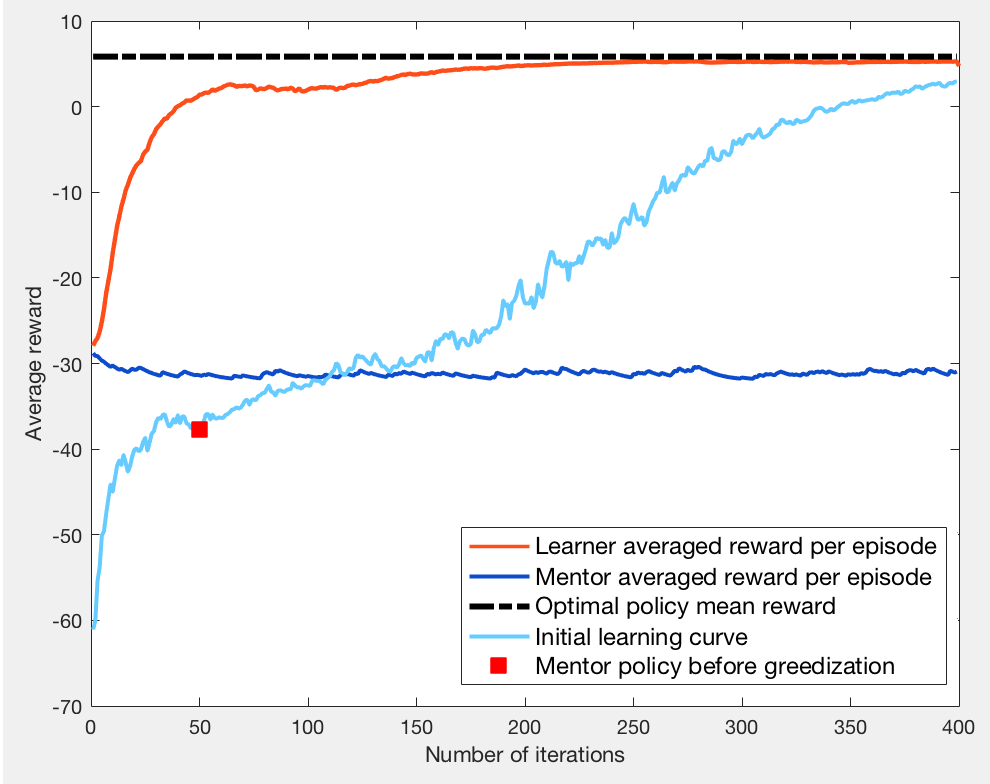
\includegraphics[width=0.95\linewidth]{av_il_subopt_50}
							\caption{Explicit compliance learning curve}
							\label{fig::av_il_subopt_50}
						\end{center}
					\end{minipage}
				\end{figure}
				
				\paragraph{} Figures (\ref{fig::av_il_subopt_120}) and (\ref{fig::av_il_subopt_50}) show the learning curves for an agent using the action-value compliant-based method, with two different suboptimal teachers. As for the $\beta$-implicit method, we are able to reduce or even suppress the undershoot that the vanishing compliance method displayed, and to obtain fast convergence. 				
			}
			\subsection{Discussion}
			{		
				\begin{figure}[ht!]
					\begin{minipage}{0.45\linewidth}
						\begin{center}
							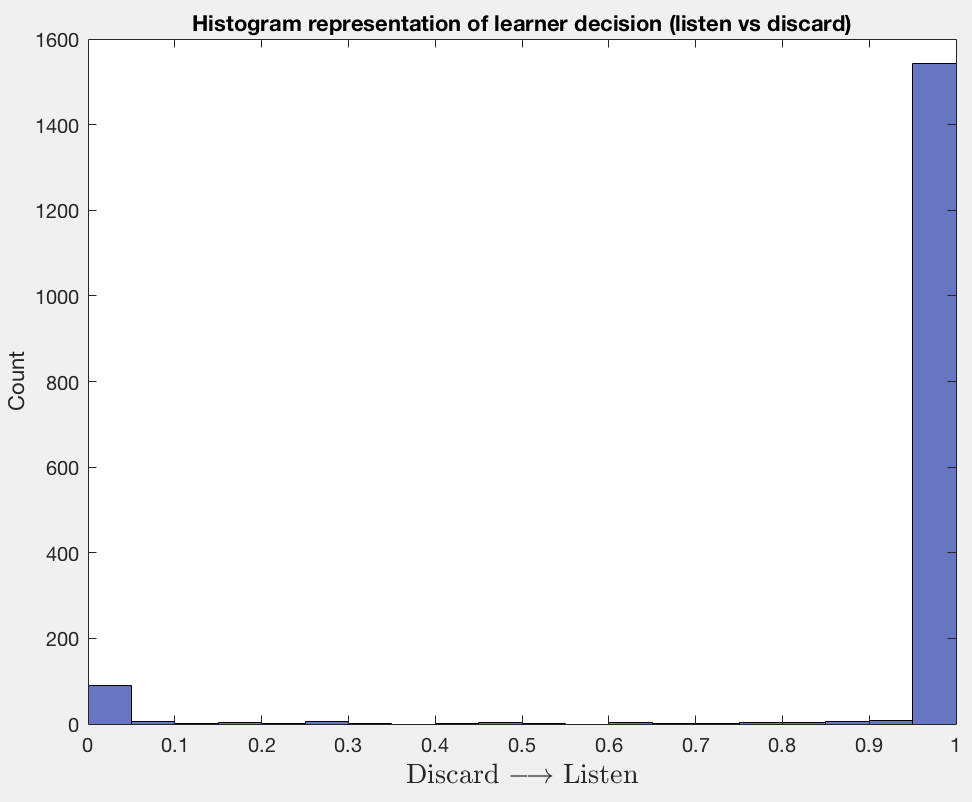
\includegraphics[width=0.9\linewidth]{pos_des_120}
							\caption{Histogram representation of the posterior decisions for a suboptimal teacher (first mentor)}
							\label{fig::post_des_120}
						\end{center}
					\end{minipage}
					\hfill
					\begin{minipage}{0.45\linewidth}
						\begin{center}
							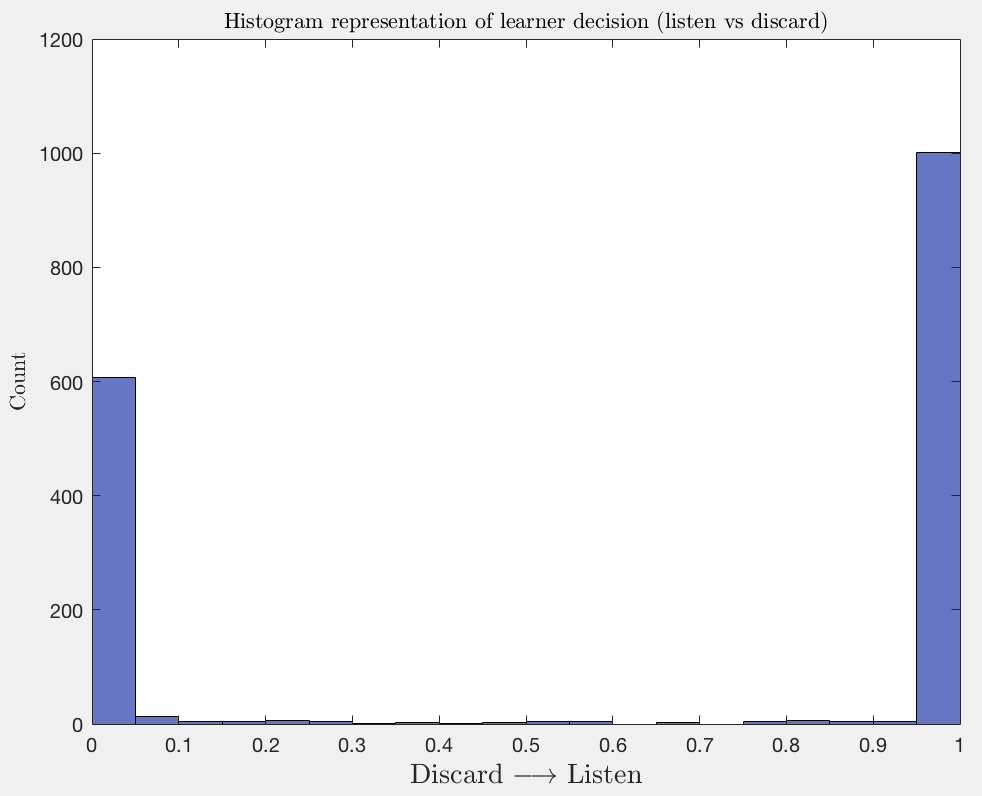
\includegraphics[width=0.9\linewidth]{pos_des_50}
							\caption{Histogram representation of the posterior decisions for a suboptimal teacher (second mentor)}
							\label{fig::post_des_50}
						\end{center}
					\end{minipage}
				\end{figure}
				
				
				\begin{figure}[ht!]
					\begin{minipage}{0.5\linewidth}
						\begin{center}
							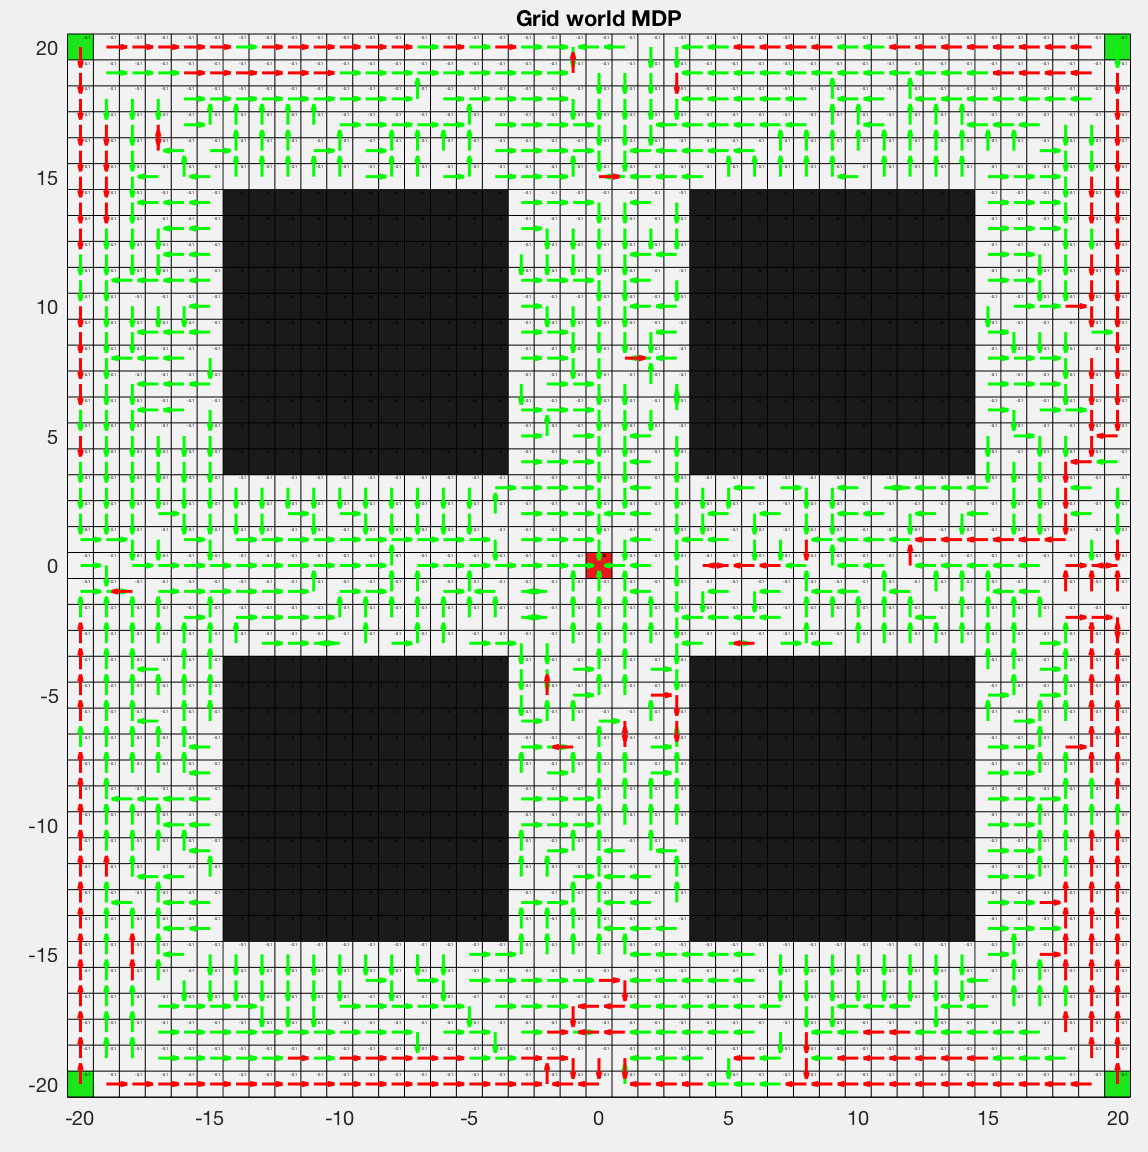
\includegraphics[width=0.9\linewidth]{heatmap_decision_120}
							\caption{Learnt decisions: green arrows show listening, red arrows discarding}
							\label{fig::heatmap_des_120}
						\end{center}
					\end{minipage}
					\hfill
					\begin{minipage}{0.5\linewidth}
						\begin{center}
							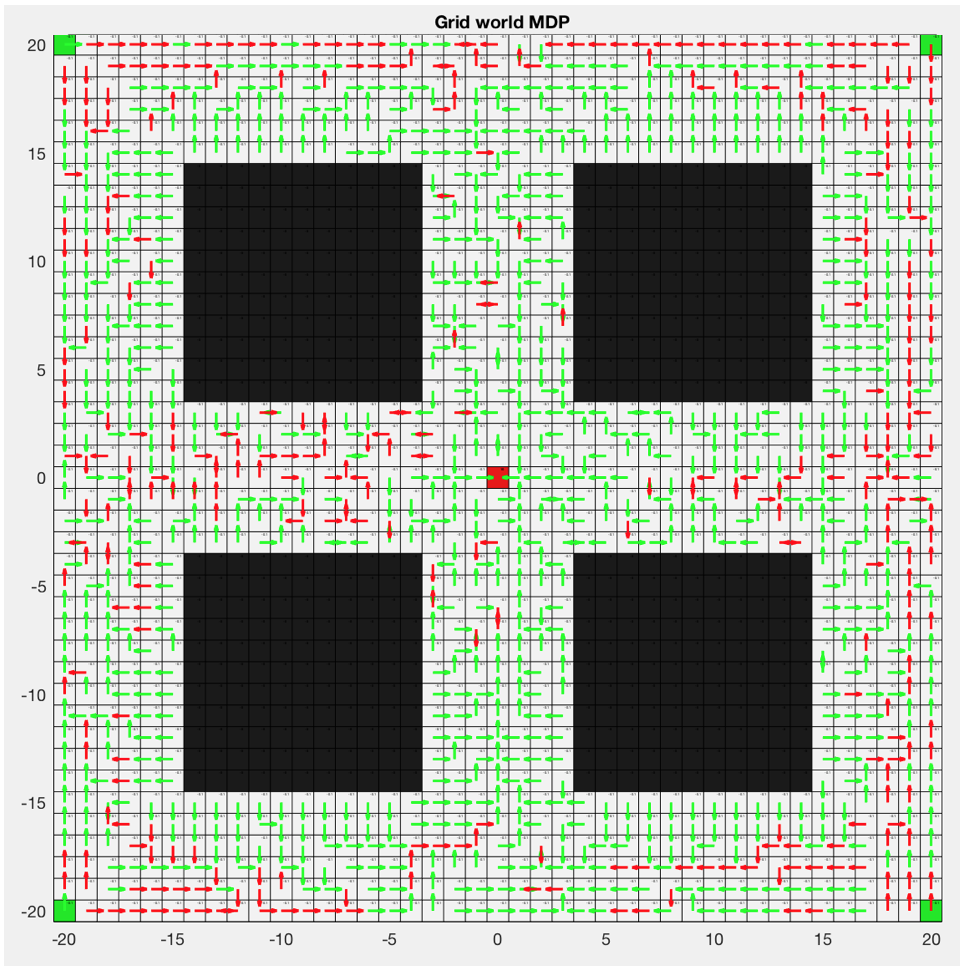
\includegraphics[width=0.9\linewidth]{heatmap_decision_50}
							\caption{Learnt decisions: green arrows show listening, red arrows discarding}
							\label{fig::heatmap_des_50}
						\end{center}
					\end{minipage}
				\end{figure}
			
			\paragraph{} Similar plots of posterior result as for the $\beta$-implicit method can now be drawn. Figures (\ref{fig::post_des_120}) and (\ref{fig::post_des_50}) display the histograms distributions for the action 'listen' and 'discard' (computed by the sigmoid value at end temperature). Figures (\ref{fig::heatmap_des_120}) and (\ref{fig::heatmap_des_50}) show the learnt decisions over the action-state space (the optimal policy is plotted, with red arrows for discarded actions and green for followed actions).
			
			\paragraph{} Again, one can see that most wrong recommandations are well-classified. However, this method as a tendency to classify an action leading to a suboptimal sequence (in the mentor's policy) as a poor action. This has for consequence that the learner will always try to go round the mentor's suboptimal recommandation, sometime by making some undesired detours. 
			}
		}
		\section{Performance comparaison}
		{
			\label{sec_method_comp}
			\paragraph{} We hereinafter focus on comparing the last three methods (vanishing compliance, implicit $\beta$-compliance and explicit compliance) between themselves and with classical reinforcement learning algorithms. 
			
			\subsection{Compliant learners}
			{
				\paragraph{} Let us now compare the different compliant learners between them. Figures (\ref{fig::compliant_comp_120}) and (\ref{fig::compliant_comp_50}) display the learning curves derived in the previous section altogether. If the $\beta$-implicit and the explicit compliance methods seem to behave better than the vanishing learner, it seems that the speed of convergence of all three algorithms tends to equalize as the teacher sub-optimality grows. As explained shortly after, this behavior is confirmed by figures (\ref{fig::metric_tt}) and (\ref{fig::metric_tr}). 
				
				\begin{figure}[ht!]
					\begin{minipage}{0.5\linewidth}
						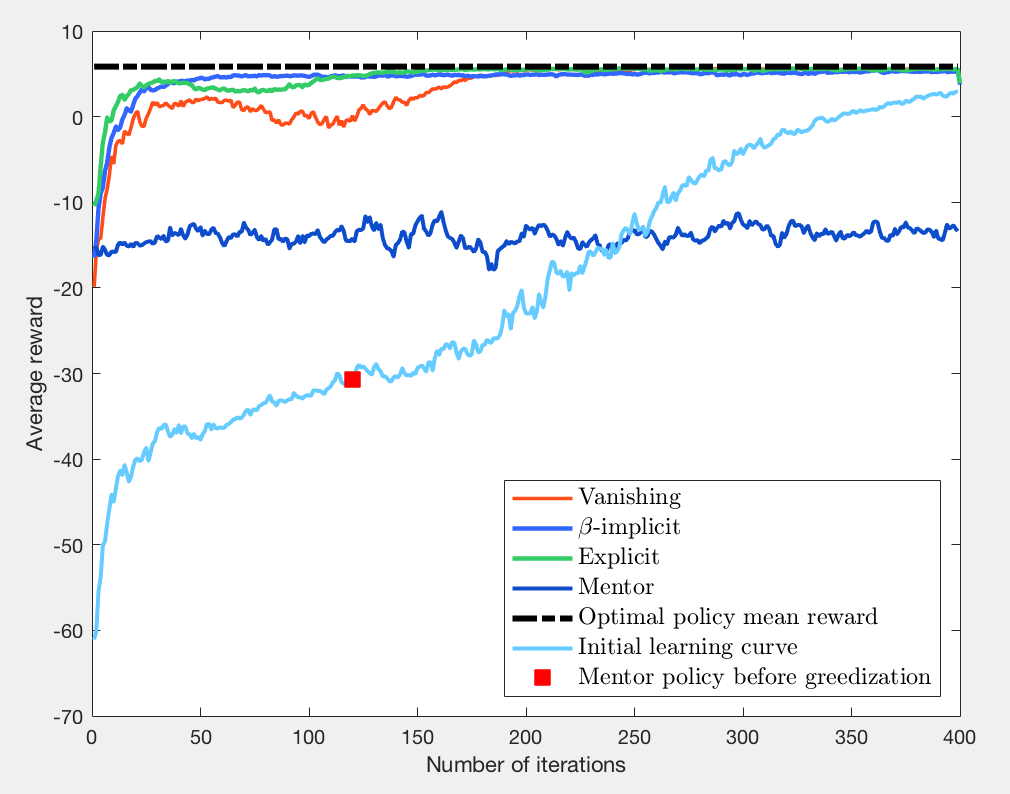
\includegraphics[width=\linewidth]{fullcomp_subopt_120}
						\caption{Learning curves for a first teacher}
						\label{fig::compliant_comp_120}
					\end{minipage}
					\begin{minipage}{0.5\linewidth}
						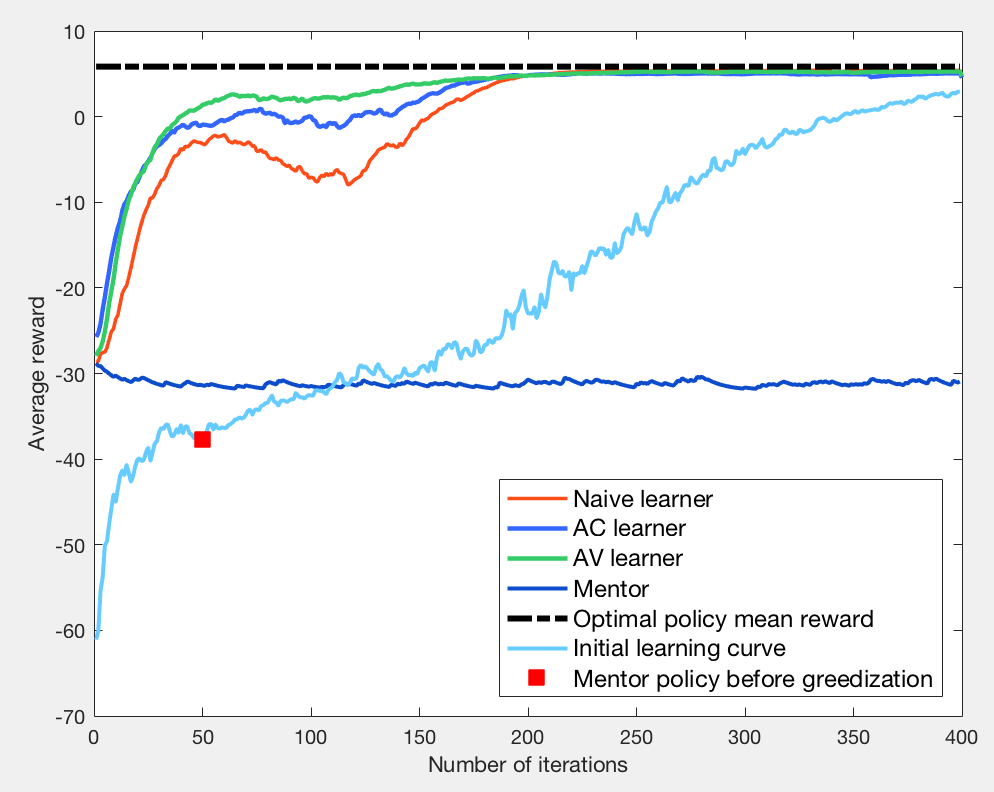
\includegraphics[width=\linewidth]{fullcomp_subopt_50}
						\caption{Learning curve for a second teacher}
						\label{fig::compliant_comp_50}
					\end{minipage}
				\end{figure}
				
				\paragraph{} We now derive some more precise metrics to assess the performances of our different algorithms. We will focus on two different metrics: 
				\begin{itemize}[label=$\cdot$]
					\item \textbf{Time to convergence}: as its name indicates, we here measure how many iterations it took for the tested algorithm to reach convergence. We define convergence as a threshold value over which the accumulated reward on one episode will stay superior to. This threshold is set to be close to the optimal policy accumulated reward on one episode (99\% of its value). 
					\item \textbf{Accumulated reward ratio}: this metric measure how the learner behaves until convergence. It computes the ratio between the reward accumulated by the learner until convergence (see above) and the reward the optimal policy would have accumulated over the same period of time. Therefore, the quickest a learning curves goes near the optimal reward, the better this metric would be. 
				\end{itemize}
				 In figures (\ref{fig::metric_tt}) and (\ref{fig::metric_tr}), different teachers are being tested based on their optimality level. This scalar measure of optimality is computed from a linear scaling between the random policy and the optimal policy mean expected return on one run. As one can see, the time to convergence metric seems to equalize for all methods as the optimality of the teacher decreases. However, the accumulated reward ratio is always better for the two adaptive methods - traducing the absence of the undershoot and better behaving methods. Hence, if our adaptive algorithms can't always speed up the learning (compared to a naive compliant learner), they \emph{provide better behaving agents}. 
				
				\begin{figure}[ht!]
					\begin{minipage}{0.5\linewidth}
						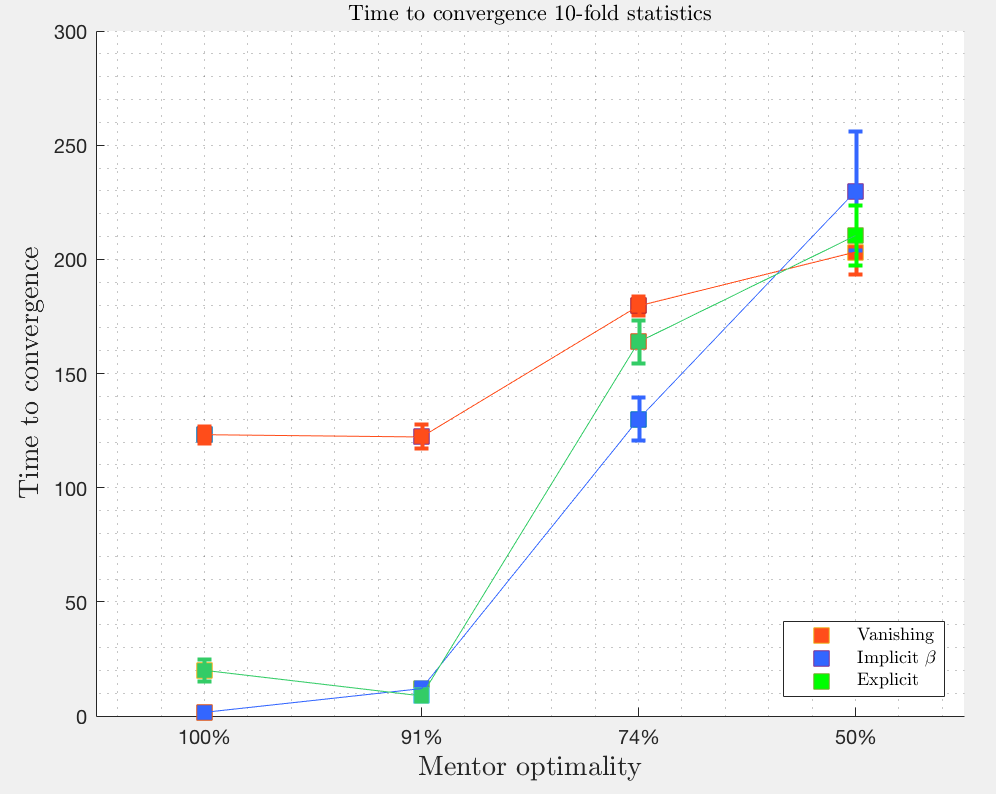
\includegraphics[width=\linewidth]{tt_metric}
						\caption{Time to convergence metric}
						\label{fig::metric_tt}
					\end{minipage}
					\begin{minipage}{0.5\linewidth}
						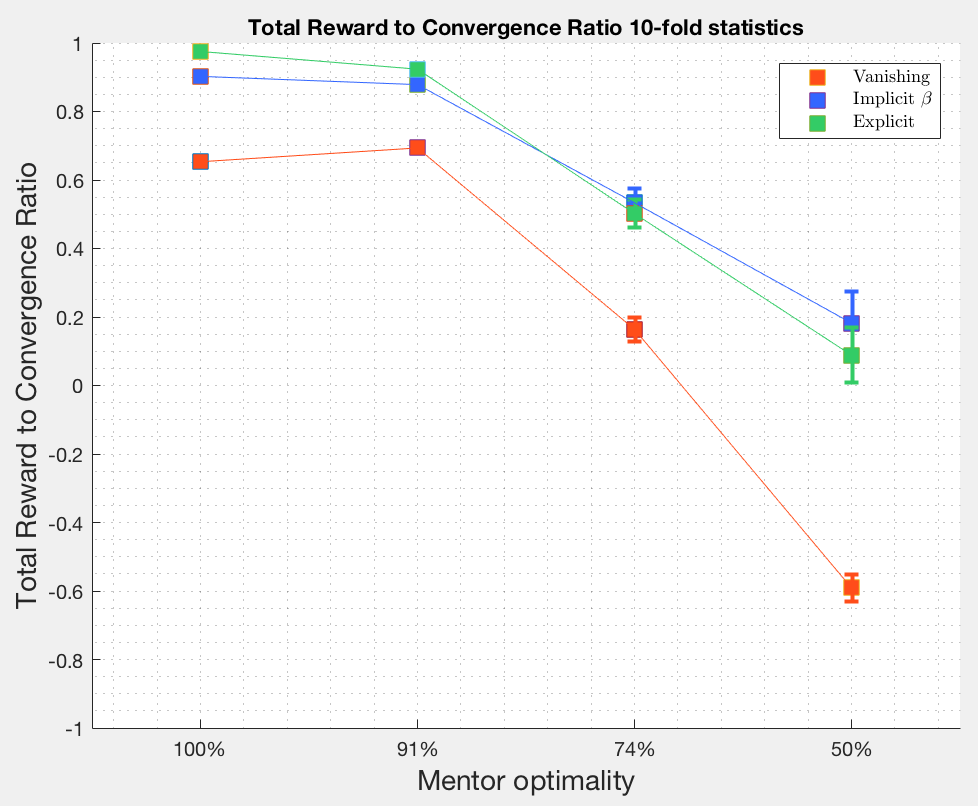
\includegraphics[width=\linewidth]{tr_metric}
						\caption{Reward ratio to convergence metric}
						\label{fig::metric_tr}
					\end{minipage}
				\end{figure}	
			}
		}
		\subsection{Classical learners}
		{
			\paragraph{} As reminded in the beginning of this document, one of the goals of learning to demonstration is to speed up the learning. The goal of this section is to compare the behavior of the compliant-based learners we developed with some more classical reinforcement learning. 
			
			\paragraph{} Figures (\ref{fig::loner_comp_50}) and (\ref{fig::loner_comp_120}) display the learning curves of the compliant learner opposed with, respectively, TD(0) learners and TD($\lambda$) learners. As one can see, our algorithms performs way better than TD(0) learners, even with largely suboptimal teachers. However, they performed as well or even slightly worse than TD($\lambda$) learners. This phenomenon is mostly due to the fact the behind its action selection, our learners update their Q-values thanks to SARSA updates (on-policy). Generalizing to an off-policy update, and eventually by making use of eligibility traces will most likely improve the learning speed and beat TD($\lambda$) learners. 
							
				\begin{figure}[ht!]
					\begin{minipage}{0.5\linewidth}
						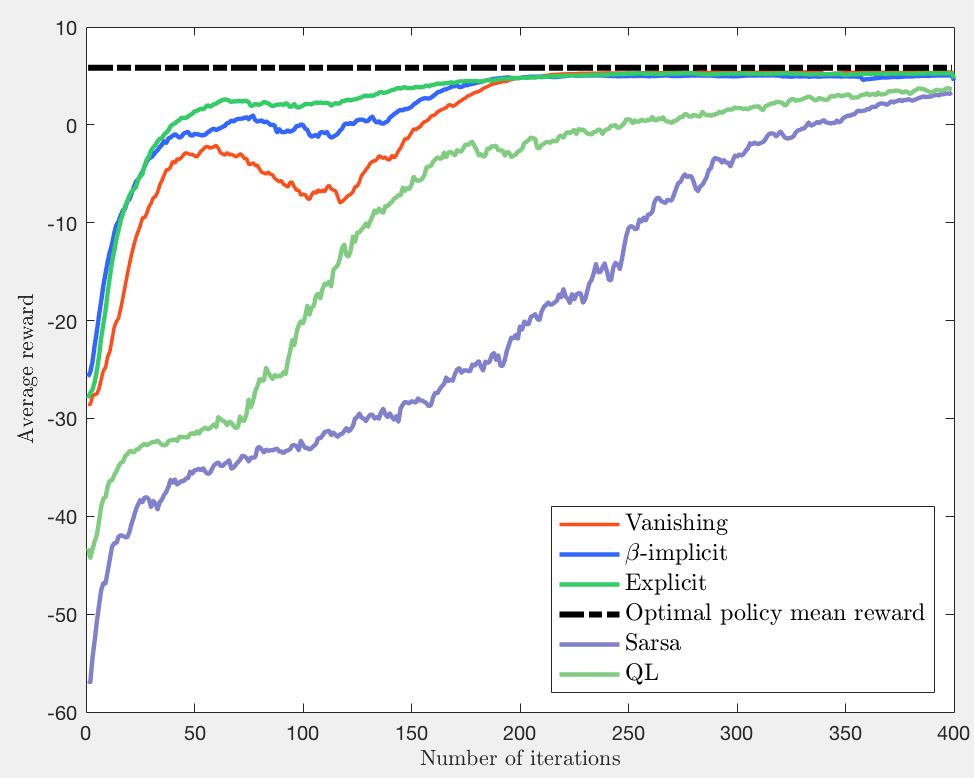
\includegraphics[width=\linewidth]{loner_comp_50}
						\caption{Method comparaison (teacher optimality: 50\%)}
						\label{fig::loner_comp_50}
					\end{minipage}
					\begin{minipage}{0.5\linewidth}
						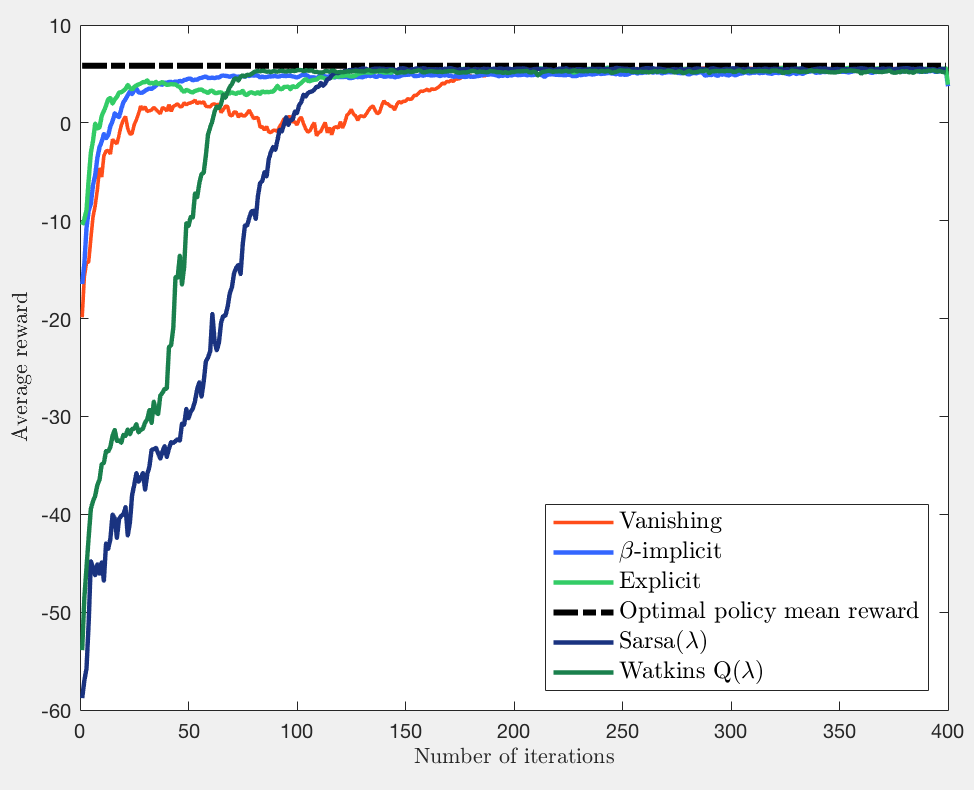
\includegraphics[width=\linewidth]{loner_comp_120}
						\caption{Method comparaison (teacher optimality: 75\%)}
						\label{fig::loner_comp_120}
					\end{minipage}
				\end{figure}
				
				\paragraph{} Figures (\ref{fig::tt_metric_w_loners}) and (\ref{fig::tr_metric_w_loners}) display the previously define metric values for both compliant learners and some different classical reinforcement learning algorithms. On (\ref{fig::tt_metric_w_loners}), we only display the result for eligibility traces algorithms, since SARSA and Q-learning have much higher convergence times than the other considered algorithms. 
				
				\begin{figure}
					\begin{minipage}{0.5\linewidth}
						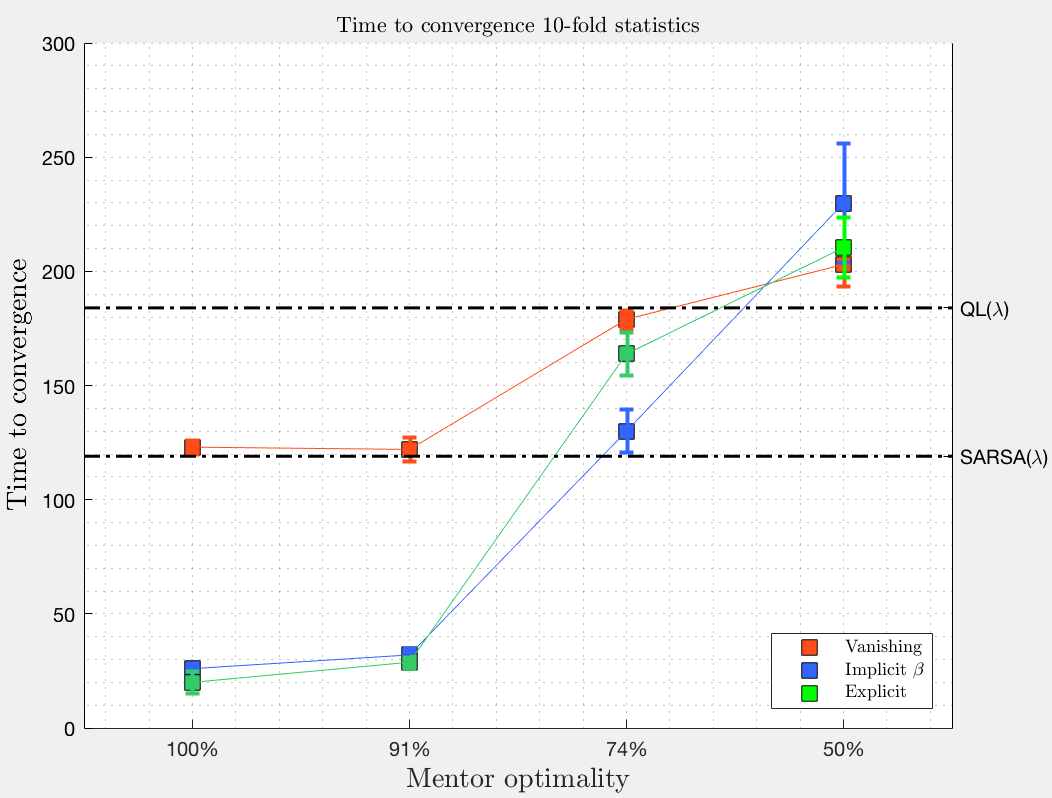
\includegraphics[width=\linewidth]{tt_metric_w_loners}
						\caption{Time to convergence metric: comparaison with classical RL algorithms}
						\label{fig::tt_metric_w_loners}
					\end{minipage}
					\begin{minipage}{0.5\linewidth}
						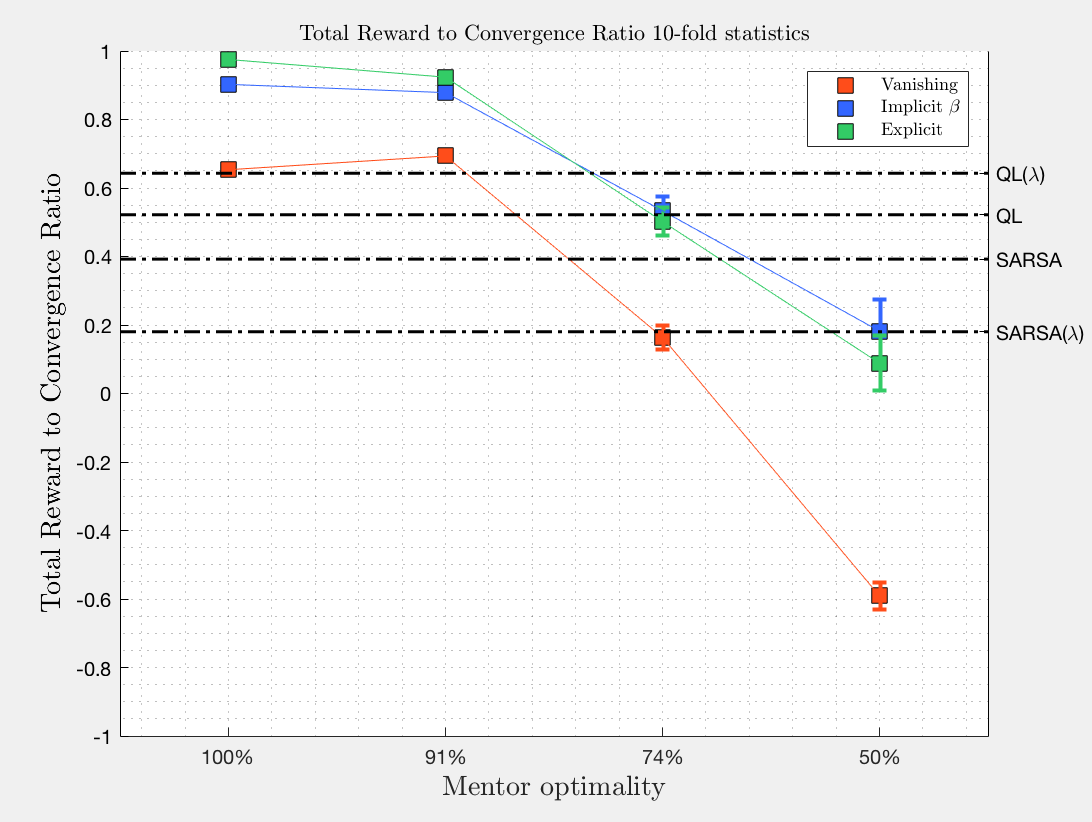
\includegraphics[width=\linewidth]{tr_metric_w_loners}
						\caption{Reward ratio to convergence metric: comparaison with classical RL algorithms}
						\label{fig::tr_metric_w_loners}
					\end{minipage}
				\end{figure}
				
			\paragraph{} Those figures confirm the fact that our compliant based algorithms have comparable performance than eligibility traces based reinforcement learning algorithms. This is rather pleasing, knowing that our update are tailored by TD(0) updates. When compared to TD(0) learners (like SARSA or Q-learning), it is clear that our compliant-based learners perform equally or better (depending on the metric). This is reassuring, since they have a significant advantage: the prior knowledge given by the mentor's demonstration. 
		}
		
		\section{Improvements}
		{
			\paragraph{} We've discussed earlier how the final result of our learning algorithms depended on the mentor. Because we are  learning on-policy, the mentor sub-optimalities have a tendency to repeal the learner from suboptimal zones, dedicating a consequent amount of time to exploration. 
			
			\paragraph{} Hence, most of the time, the learner overcomes its mentor sub-optimality only by \emph{avoiding regions where this one is sub-optimal}, instead of deciding to explore those regions and \emph{fixing the mentor sub-optimality}. This could be avoided by using off-policy learning. 
			
				\begin{figure}[h!]
					\begin{minipage}{0.5\linewidth}
						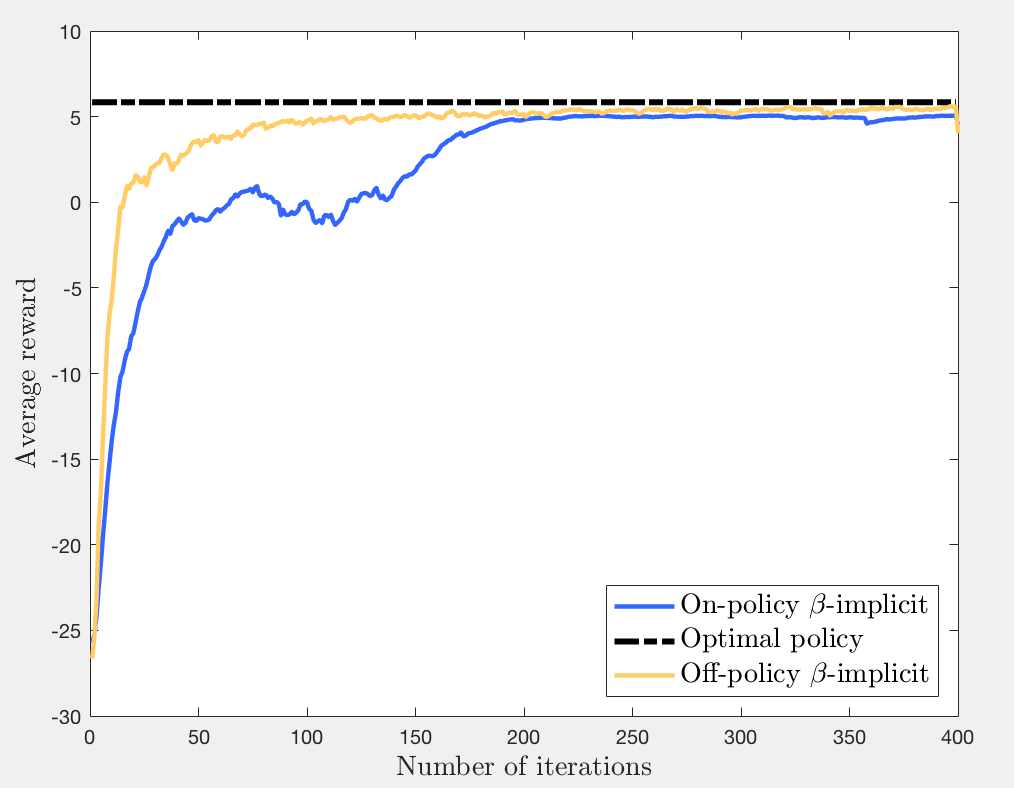
\includegraphics[width=\linewidth]{off_policy_implicit}
						\caption{Learning curves for both off an on-policy compliance-implicit learner}
						\label{fig::off_policy_implicit}
					\end{minipage}
					\begin{minipage}{0.5\linewidth}
						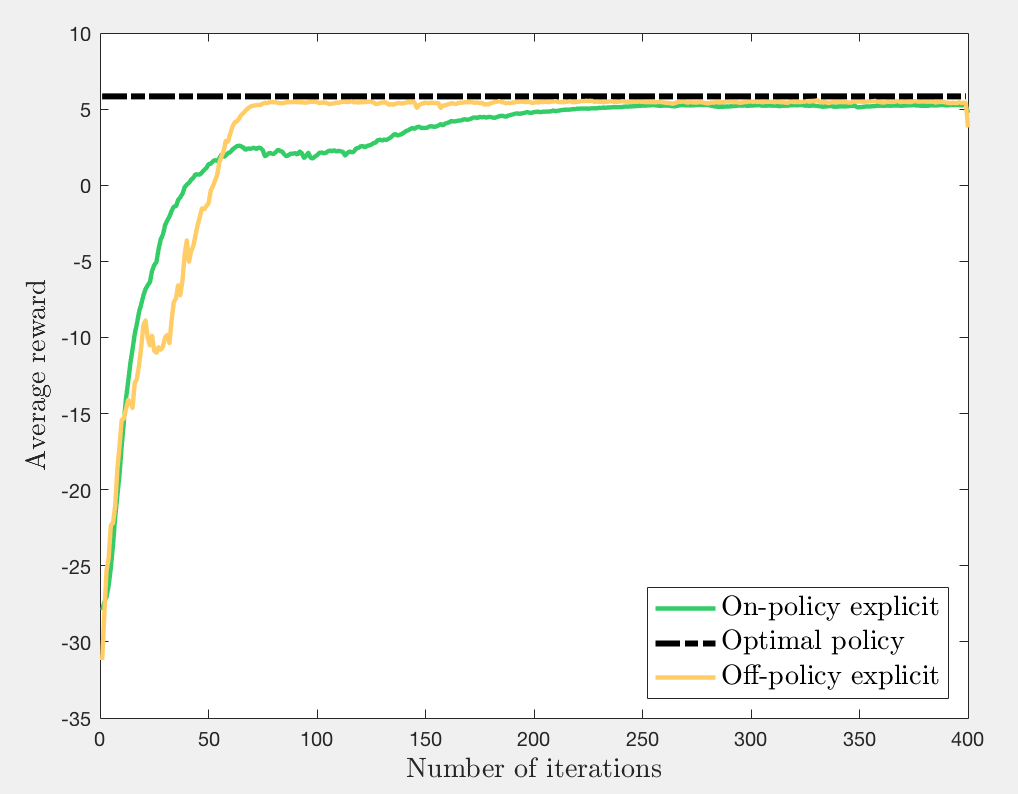
\includegraphics[width=\linewidth]{off_policy_explicit}
						\caption{Learning curves for both off an on-policy compliance-explicit learner}
						\label{fig::off_policy_explicit}
					\end{minipage}
				\end{figure}
				
			\paragraph{} The effect of learning off-policy are only noticeable when applied to largely suboptimal mentors - or more precisely, to mentors giving poor recommandations in large regions of the state space. Figures (\ref{fig::off_policy_implicit}) and (\ref{fig::off_policy_explicit}) display the learning curves of off-policy versions of our adaptative compliance methods for such a sub-optimal teacher, and compares then to their on-policy version. If it is clear that the general behavior of the learner is improved (most of the learning is done much quicker), the time to convergence is also slightly improved . If there is some incompressible time needed for exploring around the teacher's sub-optimalities, this method seems to find quicker an optimal way of doing so. 
			
			\paragraph{} As previously stated, the benefit of compliant off-policy learning is only noticeable for some special kind of mentor sub-optimalities. It is therefore a fairly good approach to treat systematically sub-optimal teachers, regardless of their level optimality. However, there is a certain level of sub-optimality (for instance, near random mentor) for which this method will tend to perform equally to the on-policy compliant learning. Again, most of the advantages of using off-policy learning in this context is that the correspoding learner will try to fix the mentor's action in some suboptimal subspace region, instead of trying to bypass it. 
				
		}
	}
	
	\chapter{Conclusion}
	{
		\section{Outline}
		{
			\paragraph{} We presented in this report a few attempts at generating compliant exploratory policies with respect to a generalized teacher demonstration. We first introduced a naive method, called \emph{vanishing compliance}, where a learner first follows its mentors recommandation before slightly taking its own decision, to eventually exploiting only its Q-values to move along its state space. We then introduced two adaptative compliance methods, learning a measure of their mentor optimality. One provides a prior to a point based confidence measure ($\beta$-implicit), while the other drives the exploration based on the learnt values of listening or discarding the teacher (explicit compliance).
			
			\paragraph{} We then evaluated those methods, focusing on their convergence speed as well as on their general behavior. When it comes to convergence speed, adaptative learners tends to performs well better than the naive learner, provided a well-behaving teacher. As the mentor's optimality level decreases, the performance of those methods tends to equalize. 
			\newline However, adaptative methods constantly displays better behavior (in terms of average rewards in a reinforcement learning vocabulary) than the naive one, which can be of consequent advantage for real world implementations. The following table sums-up the advantages and drawbacks of the three different methods displayed in this report. 
			
			\begin{center}
				\begin{tabularx}{\textwidth}{|X|X|X|}
					\hline
					\textbf{Method} & \textbf{Advantages} & \textbf{Drawbacks}\\
					\hline
					\multirow{3}{*}{Vanishing Compliance} & Easy to implement & Delicate tuning\\
												   & Systematic & Learning curve undershoots \\
												   & & No inference over the mentor's optimality level \\
					\hline
					\multirow{3}{*}{$\beta$-implicit compliance} &  Intuitive tuning & Harder to implement \\
													  & Infers the mentor's optimality level & Prior must be well defined \\
													  & Quickly reaches suboptimal level & Convergence rates are highly impacted by the quality of the mentor \\ 
					\hline
					\multirow{3}{*}{Explicit compliance} &  Easy to implement &  Convergence rates are highly impacted by the quality of the mentor \\
					& Infers the mentor's optimality level  & \\
					& Quickly reaches suboptimal level  & \\
					\hline
				\end{tabularx}
			\end{center}
			
			\paragraph{} Using rather basic reinforcement learning updates (SARSA), all three of our methods compete with the performances of more sophisticated algorithms (eligibility traces for instance), even with teachers of questionable optimality levels (in our experiment, nearly-optimal teachers have optimality levels approaching 100\% by only a few percentage). What's more, they clearly outperform the algorithms they rely on when those ones are implemented without demonstrations. However, some consequent work is left to be done in order to be able to generalize those algorithms to more complicated environments or to weaker hypothesis. 
		}
		\section{Applicability}
		{
			\paragraph{} Because the final goal of this approach concerns the application to real world problems, the question of applicability arises. Since our approach only modifies a rather small aspect of reinforcement learning, the question of its applicability actually reports to the question of applicability of reinforcement learning itself. Because of the greediness of reinforcement learning (be it computationally or in terms of the quantity of data it needs to learn), this has been quite an important topic over the last years, with some interesting results (see \cite{hester2017learning} or \cite{fastrlslowrl}). If reinforcement learning has already been implemented on simple robots, complex robotics tasks that will motivate the use of our approach are still not solvable (at least in a reasonable time) with reinforcement learning. 
			
			\paragraph{} Hence, if an attempt shows to be particularly successful, we believe that our approach could show some interesting results - since it aims at speeding up learning. Also, because our approach only deals with the steering of the exploratory policy toward a certain direction, convergence proofs still hold as long as the exploratory policy is greedy in limit. However, this last assumption is arguable for real world implementations, since no proof of convergence exists for continuous reinforcement learning. 
		}
		\section{Future work}
		{
			\paragraph{} There is still a consequent work to be done to be able to consider applying our approach to real human demonstrations. We hereinafter state the ones that seems the most important to reach an applicable level of performance and comply with real world constraints. 
			\begin{itemize}
				\item Evaluate the outcome of the methods for sparse demonstrations. Indeed, we considered in this work that a demonstration consisted of the observation of deterministic policy over the whole state space. Generalizing our approach to \emph{sparser} model of demonstration seems like an essential step. 
				\item Evaluating the effect of using eligibility traces in our learning could also be important in an attempt to increase the convergence rate. 
				\item The question of learning the prior (for the $\beta$-implicit method) or the initialization (for the explicit method) could also be of importance. Indeed, choosing a coherent prior for a given teacher highly impacts the rate of convergence. 
			\end{itemize} 
		}
		
		\section{Acknowledgments}
		{
			\paragraph{} I deeply thank Mahdi Khoramshahi and Andrew Sutcliffe for their sound advice all along this semester project. I learnt a lot under their guidance and greatly appreciated working with them. I also wish to thank Professeur Billard and the whole LASA team for their advice and bibliographic suggestions during the mid-term presentation. 
		}
	}
	
	
	
	\bibliographystyle{ieeetr}
 	 \bibliography{bibfile}
  	\nocite{*}
	
\end{document}